\documentclass[12pt]{article}
\usepackage{class_notes}
\usepackage{hyperref}
\usepackage{booktabs}
\usepackage{array} % for better arrays (eg matrices) in maths

\hypersetup{
    colorlinks=true,
    linkcolor=blue,
    filecolor=magenta,      
    urlcolor=cyan,
}
\urlstyle{same}
\graphicspath{ {figures/} }
\def\dbar{{\mathchar'26\mkern-12mu d}}

\begin{document}
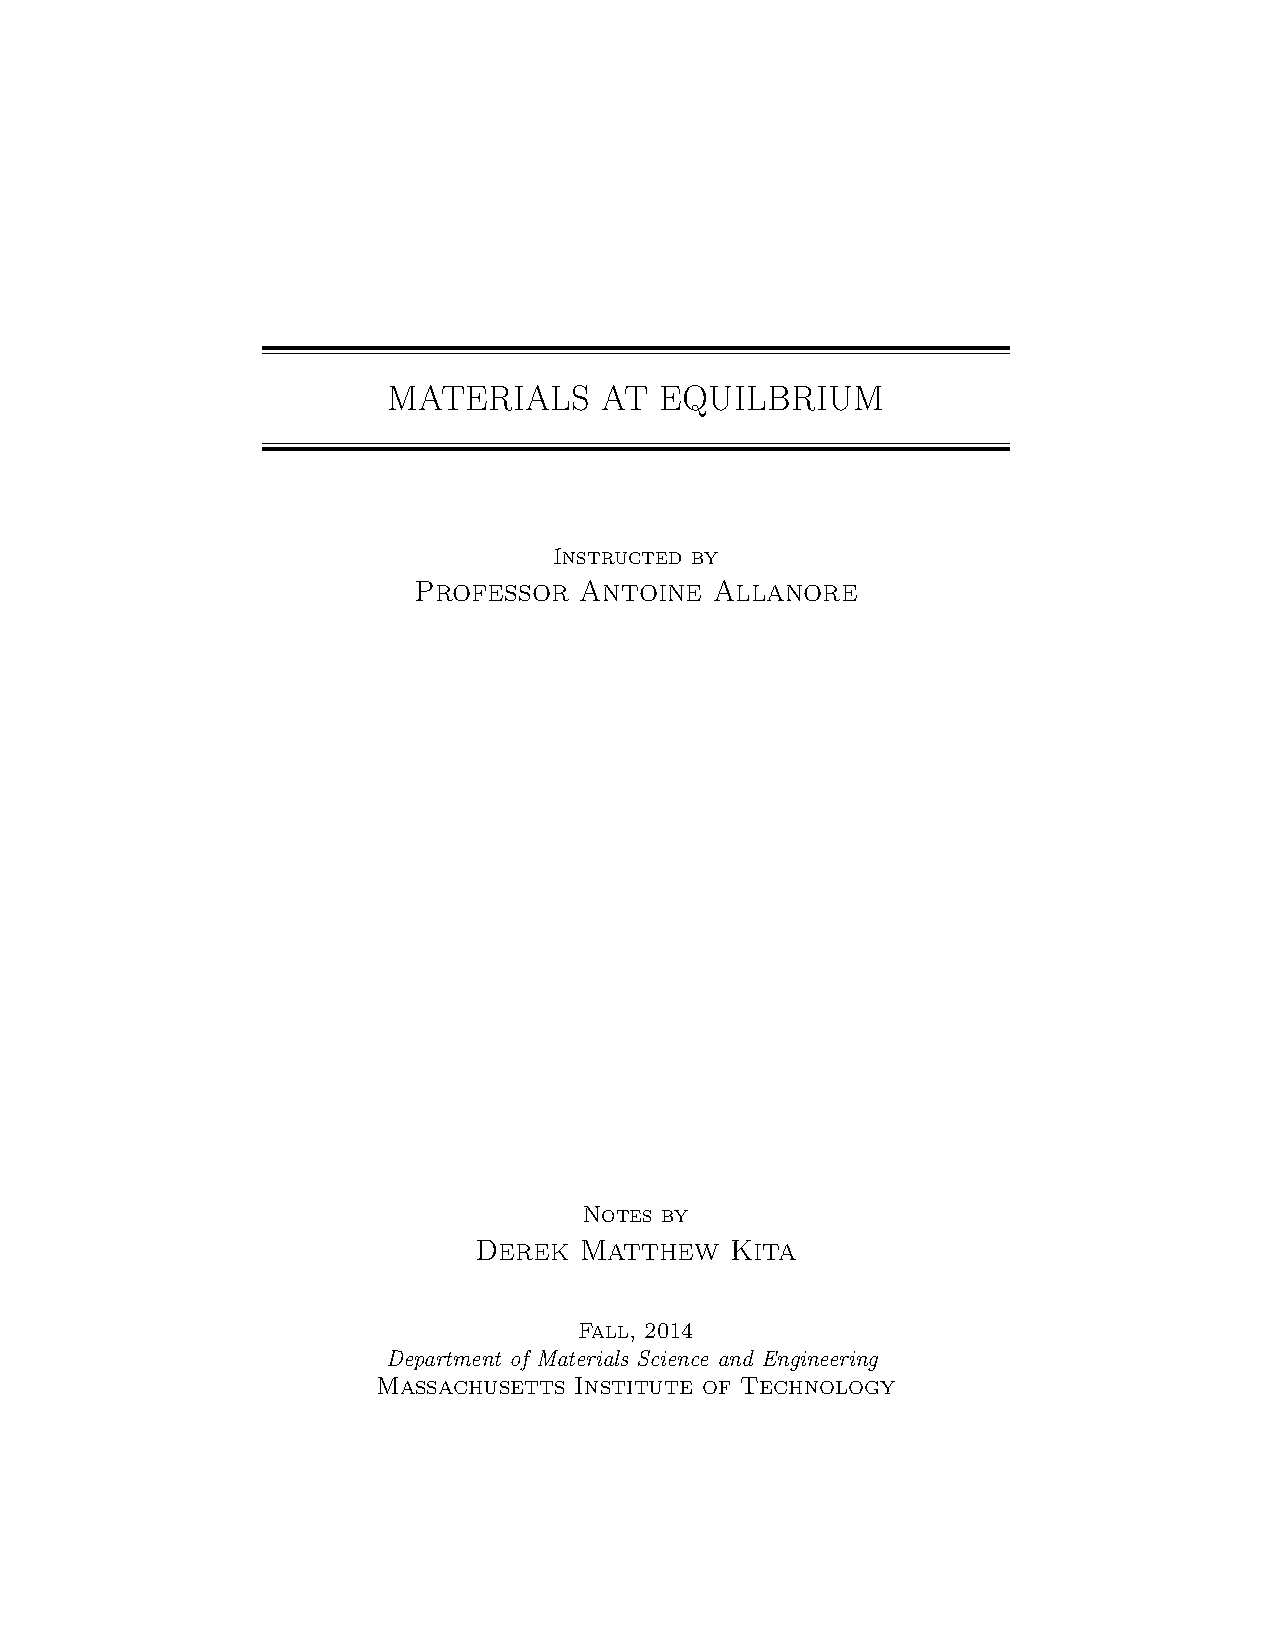
\includepdf[pages=-]{titlepage.pdf}
%%%%%%%%%%%%%%%%%%%%%%%%%%%%%%%%%%%%%%%%%%%%%%%%%%%%%%
\section{Lecture 1: Introduction and Preliminaries}
%This is an inexact differential: $\dbar$

Welcome to 3.20, Materials at Equilibrium.  This course is designed to provide all incoming students with a grounding in equilibrium thermodynamics and an understanding of energy scales.  The material in this course is broadly applicable to all field of materials science and engineering and will serve you well throughout your research as a graduate student.  For information related to the course, including lecture content, problem sets, exams, staff policies, and grading please refer to your course syllabus found on Stellar, or contact the professor directly at \texttt{allanore@mit.edu}.

\subsection{Definitions}
To begin our journey, we will define some frequently used terms for convenience.

\begin{enumerate}
\item \un{System}: Any collection of matter that can be uniquely identified and on which you can define macroscopic averages (a system is not necessarily homogeneous)
\item \un{Environment}: The complement of a system. Together, the system being studied and it's environment make up the universe. 
\eqs
\text{[environment]} = \text{[universe]} - \text{[system]}
\eqe
\item \un{Extensive Variables}: Variables that scale with the system size (i.e. volume, mass, number of particles, $n_{e^-}$, etc.).  If we bring two containers together, the volume is a sum of the individual volumes:
\begin{equation}
V = V_1 + V_2
\end{equation}
\item \un{Intensive Variables}: Variables that are independent of the system size. Intensive variables do \emph{not} scale with system size (i.e. pressure, temperature, E-field, etc.).  For example, the sum of two system's pressures is not equal to the pressure of the sum of both systems:
\eqs
P \neq P_1 + P_2
\eqe
\item \un{State Variables}: The variables required to fully characterize a system (T, P, n, ...).  These are \emph{not} equal to the \bold{state} of a system. However, at equiliibrium, there is a one-to-one mapping between the macroscopic state of the system and the full set of state variables; the state variables fully define the macroscopic equilibrium state.
\item \un{Boundaries}: Conditions that are defined for a system.  These strongly depend on the system of interest. Boundaries can have properties such as: permeable (open to mass flow, changing $n$), impermeable (closed to mass flow), adiabatic (closed to heat flow), diathermal (open to heat flow), rigid (constant volume), deformable, etc. The nature of the boundary defines how the system's state variables can change as it is subjected to different processes. For example, while a system with a rigid boundary is subject to possessing a constant volume during arbitrary processes, a system with a deformable boundary will, for sufficicently slow processes, have the same pressure as its surroundings.
\end{enumerate}

In thermodynamics, we will look at the transfer of energy and other extensive variables at the borders of systems as they undergo processes. Note that this approach treats the system as a black box; we have no idea what is going on microscopically inside the system. We will derive laws regarding the conservation and creation of the extensive variables. Using these laws of conservation, we will be able to define exactly how the macroscopic state of the system changes by only keeping track of what goes on at the boundaries of the system. We will then develop constitutive equations which relate changes in the thermodynamic state variables to one another during arbitrary processes. Integration of these constitutive equations is a powerful and general way to calculate changes in system processes during arbitrary processes. Last, we will use these constitutive relationships to look at a special set of processes; phase transitions, and derive laws for how the conditions under which these phase transitions should occur have to change as the boundary conditions on the system change.

\subsection{Energy and Forces}
What ``forms'' of energy do we have?
\begin{itemize}
\item \un{Potential energy:} Gravitational, electrostatic, etc.
\item \un{Kinetic energy:} Translation, rotations, etc.  
\end{itemize}
This energy can be manifest inside and outside the system.  Other examples of energies are thermal energy (from heat), electromagnetic energy, and chemical energy.
%\begin{equation}
%\Delta E = \Delta E_{ke} + \Delta E_{pe} + \Delta U
%\end{equation}
%where $\Delta U$ is the internal energy.  
For 3.20, we will assume that changes in the total energy $E$ of our system are equal to changes in thr internal energy $U$ of the system.
\begin{equation}
\Delta E = \Delta U
\end{equation}
This is tantamount to neglecting changes in the translational energy of the system as a whole. We assume that $U$ exists, that $U$ is a function of only the extensive thermodynamic variables ($U$ is a \un{state variable}), and that all types of energy exchange that can change the internal state of the system can be represented as work terms represent changes in $U$. We discuss this final assumption next.

%I am not sure 'assumption' is right for some of these; they are not all assumptions... some are implied by others... I think it is fine for teach purposes.

%%%%%%%%%%%%%%%%%%%%%%%%%%%%%%%%%%%%%%%%%%%%%%%%%%%%%%
\section{Lecture 2: Heat and Work}
Let's look at one form of energy transfer: \un{work}. A differential amount of work is equal to the force dotted with the displacement:
\eqs
\delta W = \vec{F} \cdot d\vec{r}
\eqe
The formalism for work is $\delta W_i = y_i dx_i$, where $y_i$ is the force (intensive) and $dx_i$ is the response (extensive). Combined, $(y_i, x_i)$ is a \bold{conjugate pair}.
\subsection{Two examples of work}
\bold{Example 1: Deformation of a material}: The work resulting from a change in strain energy is 
\eqs
\delta W = V \bar{\bar{\sigma}} \cdot d\bar{\bar{\epsilon}}
\eqe 
where the double overbars indicate that $\sigma, \epsilon$ are tensors.  To check the validity of this statement, we note that the stress $\sigma$ has units of [Pa]=[N/$\text{m}^2$], the strain $\epsilon$ is dimensionless, and the volume element $[\text{m}^3]$ together produce a quantity of [N$\cdot$ m] = [Joules]. We note that the shear stresses in this example are denoted by off-diagonals of $\sigma$ ($\sigma_{12}, \sigma_{13}, \sigma_{23}$).  If we consider only hydrostatic pressure, we will have $\sigma_{11}=\sigma_{22}=\sigma_{33}=-P$.
\eqs
\delta W_\text{pressure} &= V \cdot (-P) d(\epsilon_{11} + \epsilon_{22}+\epsilon_{33})\\
&= -P V (d\epsilon_{11}+d\epsilon_{22}+d\epsilon_{33})
\eqe
We note that the strain is defined as $\epsilon_{11} \equiv \Delta l_1 / l_1^{\text{initial}}$, and $l_1 l_2 l_3 = V$, so we can substitute $V (d\epsilon_{11}+d\epsilon_{22}+d\epsilon_{33}) = dV$:
\begin{equation}
\delta W_\text{pressure} = -P dV
\end{equation}
To solve these, we need an equation of state $P(V)$ or $\sigma(\epsilon)$.  We also have
\begin{equation}
\frac{\partial \epsilon_{ij}}{\partial \sigma_{kl}} = c_{ijkl}
\end{equation}
where $c_{ijkl}$ is the generalized elastic compliance.  If our material is \un{isotropic}, then we will see that $\frac{\partial V}{\partial P}|_T = V \cdot \beta_T$ where $\beta_T$ is the isothermal compressibility - a property of the material that describes volume changes at constant temperature. Hence, using this constitutive relation, $\beta_T(P,T)$, we can define the work done upon the system. \\

\bold{Example 2: Electrical work on an isotropic dielectric medium}: The voltage between two sides of a dielectric is given by the internal electric field and the length as $V = \mathcal{E} \cdot l$.  The energy stored in this capacitor is a product of the voltage and the charge.  If the charge, $q$, changes, we can produce a work term:
\eqs
\delta W = V dq
\eqe
Also, $q=D \cdot A$ where $D$, the electric displacement, is equal to $\varepsilon_0 \mathcal{E} + \frac{\mathcal{P}}{A\cdot l}$.  $\mathcal{P}$ is the total polarization and it is normalized by the volume, $A\cdot l$. We can do some algebra to arrive at a new expression for this work term:
\eqs
\delta W &= \mathcal{E} l  \cdot d(A (\varepsilon_0 \mathcal{E} + \frac{\mathcal{P}}{lA}))\\
&= \mathcal{E}lA \cdot d(\varepsilon_0 \mathcal{E} + \frac{\mathcal{P}}{lA})\\
&= V \varepsilon_0 \mathcal{E} d\mathcal{E} + \mathcal{E} d\mathcal{P}
\eqe

Note how the $\delta W$ nicely seperates into a response that is independent of the system and one that is determined by the material properties of the system. Some energy, $V \varepsilon_0 \mathcal{E} d\mathcal{E}$, is stored even when an electric field is applied to a vacuum. We are not interested in this energy. $\mathcal{E} d\mathcal{P}$, on the other hand, is system-dependent. This is the work term appropriate to the application of an elecric field to a system. You will notice some commonalities between the mechanical work terms discussed previously and the electrical work term: both products result in units of energy, and both can be written as the product of a generalized force (an intensive thermodynamic variable, $P,\mathcal{E}$), and a generalized displacement (an extensive thermodynamic variable, $dV,d\mathcal{P}$). These traits are commmon to all work terms which appear in the internal energy. A differential amount of done upon a system can thus be written as a sum over orthogonal work terms:
\eqs
\delta W = \sum_i y_i dx_i
\eqe
where each $y_i$ represents a generalized force, and each $x_i$ represents a generalized displacement.

%We will now discuss how we derive the form of this summation of orthogonal work terms. 
You might have noticed that we were careful to define the compressibility of a system, $\beta$, over a specific path. Specifically, we defined a compressibility wherein the system was held at constant temperature, $\beta_T$. This is because the compressibility is a function of the boundary conditions under which the compression takes place. \footnote{For example, it takes more energy to compress a gas if you don't let heat flow out of the gas during the compression; the adiabatic compressibility is larger than the isothermal compressiblity.} This concept can be generalized to all work terms: \emph{the work done in changing an extensive variable is a function of the path along which the work takes place}. Put simply, the change in internal energy due to the work terms are \un{path dependent}. In thermodynamics, we make a distinction between path-dependent and path-independent intergrals via exact differentials and inexact differentials. 
\begin{itemize}
\item \un{exact differentials}: The integral of an exact differential path independent; it is only a function of the endpoints.
\item \un{exact differentials}: The integral of an inexact differential is path dependent; the integral depends both on the endpoints and the path to get to these two endpoints.
\end{itemize}
This is illustratted below with two examples.
%%%%%%Next, we can relate this quantity to the characteristic potential energy function of our system.  We know that $\Delta U = U^\text{final} - U^\text{initial}$, and $\delta W = y_i dx_i = F d\vec{r}$.  The force from a potential energy function $\phi$ is $\vec{F}(\vec{r}) = -\vec{\nabla}\phi(\vec{r})$.  Therefore, we have
%%%%%%\begin{align*}
%%%%%%F_x &= -\frac{\partial \phi}{\partial x}|_y \\
%%%%%%F_y &= -\frac{\partial \phi}{\partial y}|_x
%%%%%%\end{align*}
%%%%%%$\vec{F}d\vec{r}$ is an exact differential.  It's integral is path independent.  $\oint \vec{F} \cdot d\vec{r} = 0$.  Also, $\vec{F}$ is a conservative force.  It is like the ``vehicle'' that converts gravitational energy, $E_g$ to electricity.
%%%%%%\begin{align*}
%%%%%%\int_{r_1}^{r_2} \vec{F} d\vec{r} &= \int - \vec{\nabla} \phi(\vec{r})d\vec{r}\\
%%%%%%&= [\phi(\vec{r_2}) - \phi(\vec{r_1})]
%%%%%%\end{align*}

\subsection{Practice with Differentials}
\bold{Case 1, Exact Differentials:}
Consider heights as a function of position, $h(x,y)$.  We will travel from some height $h_1 \rightarrow h_2$.  Anytime we move downwards, we will simply gain kinetic energy.  Anytime we move up a hill, we will first use any kinetic energy we have and then use some stored energy (say, from a battery).  Once we have reached $h_2$, we will give all our kinetic energy to the environment (say from some thermal energy dissipation, like brakes) and we will allow the environment to replenish the energy in our batteries.  The change in potential energy between the two heights is $\Delta E_\text{field}$ and the energy of the environment, i.e. the work required to move us to this new spot, is $\Delta E_\text{system}$.  From conservation of energy,
\eqs
\Delta E_\text{system} + \Delta E_\text{field} = 0
\eqe
Therefore, we can calculate the work required to move us to the new spot via integration of the differential of the gravitational energy with respect to the position (the gravitational force field):
\eqs
\Delta E_\text{field} = dW &= \int \vec{F} \cdot d\vec{r}\\
& = -\int \nabla E_\text{field} \cdot dr\\
& = - mg(h_2 - h_1)
\eqe
Ultimately, the energy change (or work required to move us) from $h_1 \rightarrow h_2$ is independent of the path taken.  Hence, $\vec{F}$ is an exact differential. Mathematicians would say that gravitational force fields are conservative vector fields. This is an equivalence; exact differentials define conservative vector fields.

\bold{Case 2, Inexact Differentials:}  Consider now a system where the force $\vec{F}$ is non-conservative.  The work terms associated with moving through this kind of a vector field are then inexact differentials. \un{Dissipative forces} tend to make the force vector-field non-conservative, resulting in path dependence. For example, moving in a gravitational field with a constant friction term would result in:
\begin{align*}
\vec{F} &= -\vec{\nabla}\vec{E} - f_\text{friction} | \vec{e_v}|\\
\int \vec{F}\delta\vec{r} &= -mg\Delta h- f L_\text{path}
\end{align*} 

 In thermodynamics, you can get an inexact differential for two reasons. As described above, dissipation leads to inexact differentials. A second, related way, is simply not taking into account all of the forces during your integration. Such an incomplete description will result in path-dependent integrals, even if the underlying vector field is conservative. For example, if we are moving in three dimensions and do not describe the force in the $y$-direction, $F_y'$, then we would (incorrectly) describe the work when moving in three dimensions as:
\begin{align*}
\delta W_\text{incomplete} = \delta W_x + \delta W_z = F_x \dot dx + F_z \dot dz 
\end{align*}
Consider two different paths in a conservative 3D vector field.  The integrated amount of work done due to the x- and z- forces may be different between the two paths, even though the total work is the same. This results in a path dependence in the energy acquired while moving.  For path \#1 we might have $\int \delta W_x + \delta W_z = \int F_x dx + F_z dz = 0$ whereas for path \#2 we could very well have $W_x = \int F_x dx \neq 0$.  This is analogous to describing the changes in internal energy of a system through only work terms; we are missing an entire component of the internal energy change, the change to due to \un{heat} flow into a system.



\subsection{Heat}
Heat is energy transferred between two bodies not due to work or mass transfer\footnote{Historically, people used to think heat was transferred between bodies via the flow of an invisibile substance, \textit{phlogiston}. Hot bodies contained more of this self-repelling fluid than cold bodies. However, Antoine Lavoisier showed that metals gained mass when they oxidized, even though they were supposed to lose phlogiston, so phlogiston would need to have negative mass. This lead to phlogiston theory being replaced by caloric theory, in which calor, another invisible liquid, flowed from hot to cold bodies. All caloric theories assumed that calor was conserved. Sir Benjamin Thompson (a.k.a. Lord Rumford) disproved this theory by showing that repeatedly boring a cannon could repeatedly produce heat, showing that heat was not a conserved quantity, but rather, could be generated. This lead to Rudolf Clausius proposing that it is not heat which is conserved, but rather energy. This was the birth of modern thermodynamics.}.  The variable we will use to denote heat is $Q$.  A system surrounded by an adiabatic boundary does not transfer heat across its boundaries, and so we say the heat exhanged between the system and the surroundings is 0; $\delta Q = 0$.  The \un{first postulate of thermodynamics} is
\begin{equation}\boxed{
dU = \delta W + \delta Q
}\end{equation}
where again, the work terms can be written as $\delta W = \sum_i y_i dx_i$.The value of $U$ is path independent via the conservation of energy. As such, $U$ is a function of solely the system's state. Appropriately, functions which are completely defined by the thermodynamic state of the system are called \un{state functions}; their differentials must thus be exact differentials. On the contrary, $W$ and $Q$ are \un{path dependent}; transfer of energy can be accomplished in a multitude of ways.  This is why we write both changes in heat and work with the inexact differential symbol, $\delta$, but the sum of the two as $dU$. We illustrated this with an example:

\bold{Example:} Consider a simple system with all variables fixed except for the volume, like a piston.  It then evolves ``slowly'' through a series of equilibrium states.\footnote{We call such infinitely slow processes, wherein the system can be approximated as being in equilibrium the whole time  \un{quasistatic processes}.}  
\eqs
W = -\int P dV
\eqe
Assuming we are dealing with an ideal gas, we have the following equation of state $P = \frac{nRT}{V}$.  Inserting this into the above (and assuming constant temperature), we have an expression for work in terms of the initial and final volumes.
\eqs
W &= -nRT\int \frac{dV}{V}\\
&= nRT \ln\Big(\frac{V_f}{V_i}\Big)
\eqe
It is often useful to think of these changes as paths in a pressure versus volume plot.  Let's consider a path $a$ where both the pressure and volume can change.  We will compress the gas isothermally from a volume $V_1$ to a final volume $V_f = V_1/2$.  Also, we are at room temperature, $T=298K$.
%%%% We should insert the relevant P-V diagram here!
\eqs
W_a &= -nRT\int \frac{dV}{V}\\
&= -nRT \ln\Big(\frac{V_f}{V_i}\Big)\\
&= nRT \ln(2)\\
&= 1717 \frac{\text{J}}{\text{mol}}
\eqe
Let's now consider a separate path $b$ that is first isobarically compressed ($dP=0$), and then isochorically warmed ($dV = 0$), such that both the initial and final states are the same as those in $a$.  For the constant volume pressure change, there will be no work done since $dV=0$ and $W=-PdV$.  Therefore all the work will come from the initial constant pressure process, or isobaric compression.
\begin{align*}
W_b &= -P_i \int dV\\
&= \frac{P_i V_i}{2}\\
&= \frac{nRT}{2}\\
&= 1239 \frac{\text{J}}{\text{mol}}
\end{align*}

Clearly, the amount of work done when changing between two states can be different, although the change in internal energy must be the same. Thus, there must have been different amounts of heat transferred along each path as well; both work and heat are path-dependent.

%%%%%%%%%%%%%%%%%%%%%%%%%%%%%%%%%%%%%%%%%%%%%%%%%%%%%
\section{Lecture - September 8, 2014}
Last time, we stated the first law of thermodynamics, namely that energy can only be transferred in and out of a system as work and heat: $dU = \delta Q + \sum y_i dx_i$.  
%\subsection{Today}
We now want to quantify the first term, or \un{quantify heat exchange}.  We do this by defining the \emph{heat capacity} for a system as:  %(normalized by $n$) 

\begin{align*}
C_\text{path} (T) &= \frac{(\delta Q)_\text{path}}{dT}\\
c_\text{path} (T) &= \frac{C_\text{path}}{N} %\frac{(\partial Q)_\text{path}}{dT}
\end{align*}
where $C_\text{path}$ is the system heat capacity along a given path, and $c_\text{path}$ is the specific heat capacity; the system heat capacity divided by the number of moles, $N$.\footnote{This convention is used throughout: system quantities are uppercase, molar quantities are lowercase}   If we consider a \un{simple system}\footnote{In a simple system, work can only be done on the system via $PdV$ terms.} with state variables $(P,V)$ or $(V,T)$, we can define
\begin{align*}
c_p &= \frac{1}{N} \frac{(\delta Q)_p}{dT}\\
c_v &=  \frac{1}{N} \frac{(\delta Q)_v}{dT}
\end{align*}
as the heat capacities at constant temperature and volume, respectively. The two quantities are related; it is natural to wonder what this relationship is. %can wonder what is larger, $C_p$ or $C_v$.  
The table below shows the molar heat capacity for a set of substances.
\begin{center}
\begin{tabular}{ c|c|c } 
 %\hline
 Substance & $c_p$ (J/mol/K)& $c_v$ (J/mol/K) \\ 
 \hline
 Air (room) & 29.1 & 20.8 \\ 
 Argon & 20.8 & 12.4717 \\ 
 Carbon dioixide & 36.9 & 28.5\\
 Liquid Water & 75.3 & 74.5\\
 Octane (Gasoline) & 228 &  \\
 %\hline
\end{tabular}
\end{center}

You might notice a few things. First, that the heat capacity increases with increasing molecular weight; this is general. Next, that $c_p > c_v$ for all cases. Both of these phenomena are general. Last, you might see that $c_p \approx c_v$ for $H_2O$. This is also general for condensed phases. We will prove the generality of these statements. %A heuristic arugment is as follows: at constant $V$, $\Delta U = Q$.  At constant $P$, $\Delta U = Q + W = Q - p \Delta V$.  If you raise the temperature of the system, the amount you need to put in  $\Delta U$ and $T$ will be less.\\
You can quickly estimate heat capacities for some substances using \href{http://en.wikipedia.org/wiki/Equipartition_theorem}{equipartition theory}, wherein each degree of freedom contributes $R/2$ to the molar heat capacity:

(a) \un{Gases}: If we assume that an ideal, monatomic gas has a degree of freedom for every direction it can translate it, we get three degrees of freedom, so:
\begin{equation}
c_v^{\text{monatomic gas}} = \frac{3}{2} R = 12.471 \text{ J/mol/K}
\end{equation}
Note how close this is to the value for argon, which exists as a monatomic gas.   %$R = 8314 \text{J}/\text{mol}/\text{K}$ and $R = N_a \times k_B$.  
A diatomic gas, can be modelled as two atoms are attached by a spring, free to rotate about their center of mass. At low temperatures, this gives 2 rotational degrees of freedom in addition to the original translational degrees of freedom, so at low temperatures, the heat capacity of a diatomic gas is: $c_v^{\text{diatomic, low }T} = \frac{5}{2} R$.
at higher temperatures, the two vibrational degrees of freedom are excited, giving: $c_v^{\text{diatomic, high }T} = \frac{7}{2} R$
This is borne out in the experimental data, as shown in Figure \ref{CPofgases}:
\begin{figure}[h]
\centering
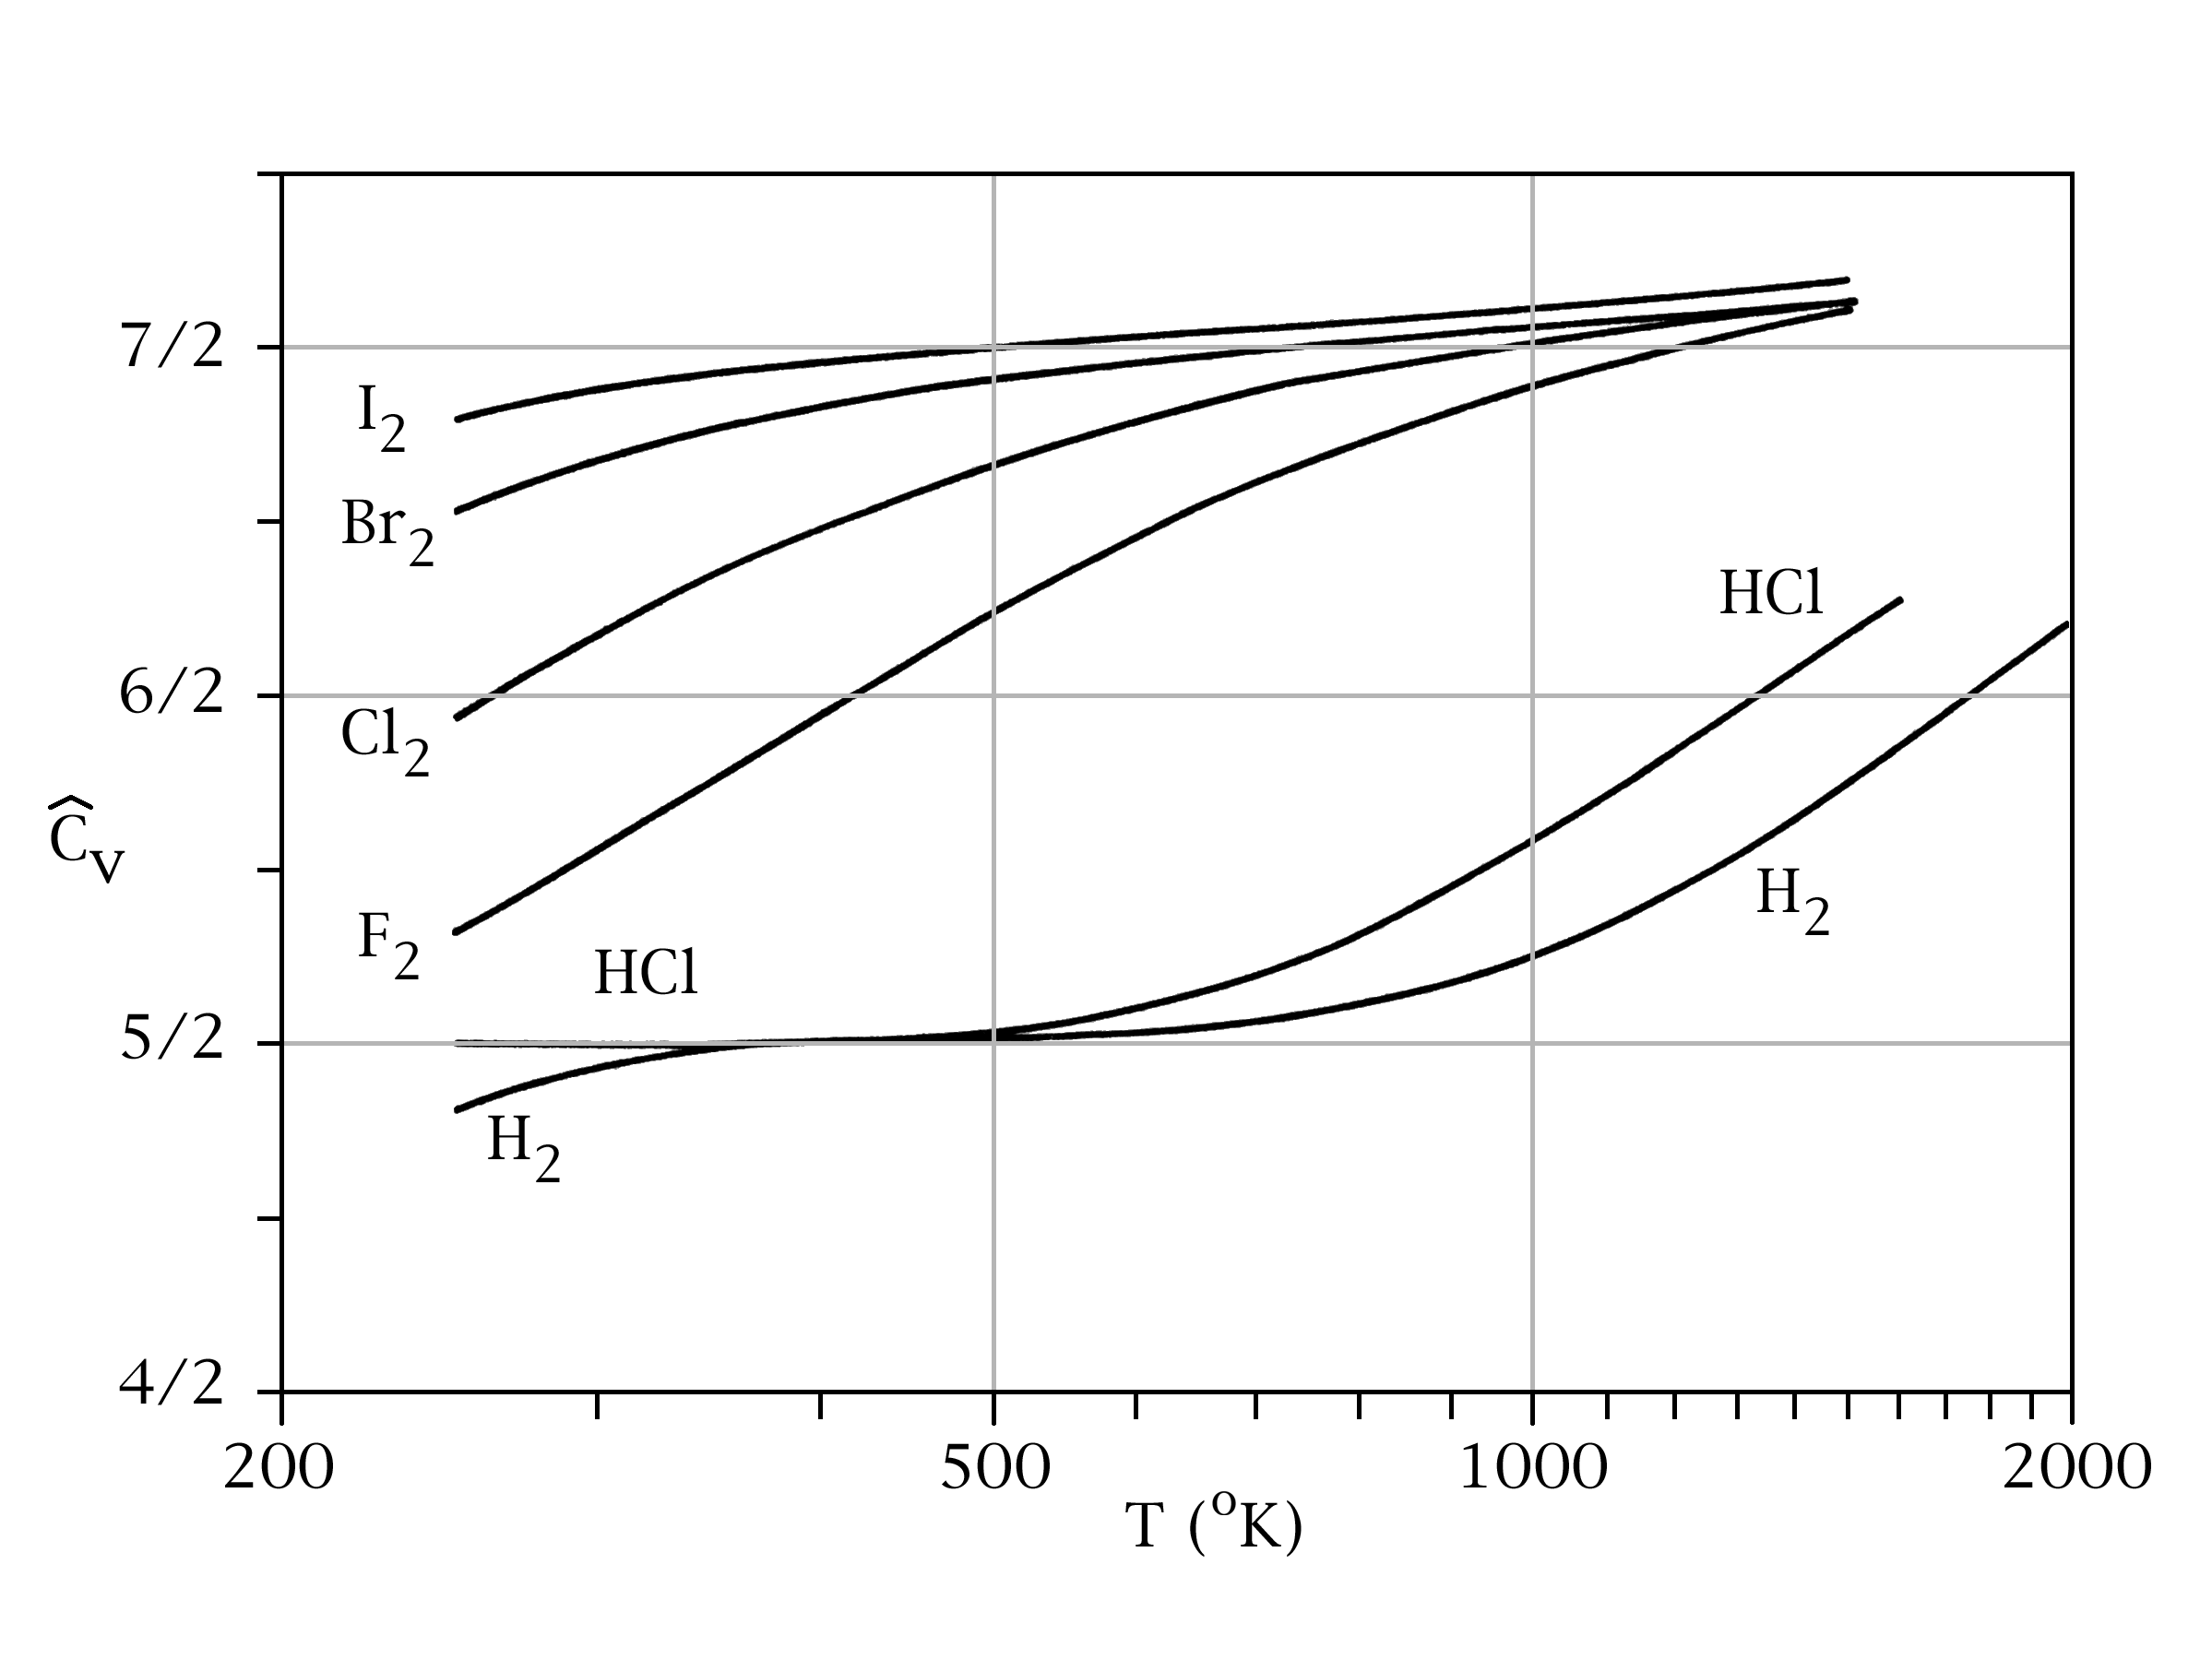
\includegraphics[width=\textwidth]{DiatomicSpecHeat2}
\caption{The specific heats of diatomic gases (normalized by R) as a function of temperature. The temperature at which the vibrational modes are excited is a function of the stiffness of the bond, with hydrogen exhibiting especially stiff bonds, and thus a late transition temperature.}
\label{CPofgases}
\end{figure}

\begin{align*}
C_p &= C_v + R\\
&= \frac{7}{2} R =  29 \text{J}/\text{mol}/\text{K}
\end{align*}


(b) \un{Solids}: At room temp., for an element, Dulong and Petit (1819) observed that
\begin{align*}
C_v &\approx 3 R = 25 \text{J}/\text{mol}/\text{K}\\
C_p & \approx C_v
\end{align*}
We will talk in detail about solid-state heat capacities during statistical mechanics, but for now it is enough to know that each atom has 6 degrees of freedom for its vibrations: 3 translational and 3 positional. So, by equiparition, $c_v$ should be $~6 \frac{R}{2}=3R$. For a non-metallic salt such as Mg, there are twice as many atoms per formula unit, so $c_p \approx 6 R = 50\text{J}/\text{mol}/\text{K}$.   If we examine some measured  $c_p$, we see that at high T carbon reaches the 3 R.  It takes a while to reach this because of the nature of carbon's strong covalent bonds (we will explain this in detail in statistical mechanics as well).  There are discontinutities in Fe's diagram at 1550 \degree C because at this point it melts.  Same with Hg, which becomes a gas at low T.  For H\2O at RT we have $C_p = 75 \text{J}/\text{mol}/\text{K}$.

\subsection{We need another energy function}
While $c_v$ is naturally defined as the derivative of the internal energy with respect to temperature at constant volume: $c_v = \frac{1}{N} \left(\frac{\partial U}{\partial T}\right)_V$, the constant pressure heat capacity, $c_p$, is often what we meaure in the lab. It would be convenient to have a energy function for which $c_p$ is the derivative of the free energy with respect to temperature. The \bold{enthalpy}, $H$, is this function.
\begin{align*}
H &= U + PV\\
dH &= dU + V dP + P dV
\end{align*}
and substitute $dU = \delta Q - P dV$
\begin{align*}
dH &= \delta Q + V dP\\
(dH)_p &= \delta Q
\end{align*}
Note how the enthalpy is naturally expressed with pressure held constant than volume held constant. Because H is defined in terms of state functions, the enthalpy is also a state function. It is the state function that describes the heat change at constant pressure.  It is thus the natural energy for discussing \textbf{calorimetry}, which is a major experimental technique.  $H$ is often called the ``heat'' content.\\

If we write down what $(dH)_p$ is, we get
\begin{align*}
(dH)_p &= n C_p (dT)_p\\
\Big(\frac{\partial H}{\partial T}\Big)_p &= C_p\\
\end{align*}
If we heat a substance through a phase transition, the enthalpy of the system can be broken into three parts:
\eqs
H(T) &= H(T_0) +  \int_{T_0}^{T_f}C_p  dT + \Delta H_{\phi T}
\eqe
where the first term is the enthalpy of the system in its initial state, the second term is the contribution of the heat capacity as a funciton of temperature ignoring the phase transition, and $\Delta H_{\phi T}$ is the enthalpy due to the phase transition, often called the latent heat of the transition\footnote{For example, the solid$\to$liquid phase transition has a \emph{latent heat of melting}}.  Unlike $T$ or $P$, there technically is no absolute zero for $H$ or $U$\footnote{Only relative energies between states are physically measurable}.  As such, we often reference these state functions to their \emph{standard states}. Under the this convention, $H=0$ for a pure element at atmospheric pressure ($P_0 = 101,325$ Pa) and temperature ($T_0 = 298$ K). Note that because elements have zero enthalpy under standard conditions, compounds formed from reactions of several elements will generally have non-zero enthalpy; heat is often exchanged when a chemical reaction takes place.\\

%(H\degree(Fe))
The enthalpy as a function of temperature is plotted below for Fe over two temperature scales. The slope of these lines, $\frac{(dH)_p}{dT}$, is the heat capacity.  Below 900\degree C, Fe is in the $\alpha$ (BCC) phase, from $900^0 < T < 1400^0$ it is in the $\gamma$ (FCC) phase, and from 1400$\to$1500\degree C Fe is the $\delta$ (BCC2) phase. Above 1500\degree C , Fe melts. Fe evaporates near $2900 \degree$C. Each of these can be observed as discontinuities in the $H(T)$ curve. \\
\begin{figure}[h]
\centering
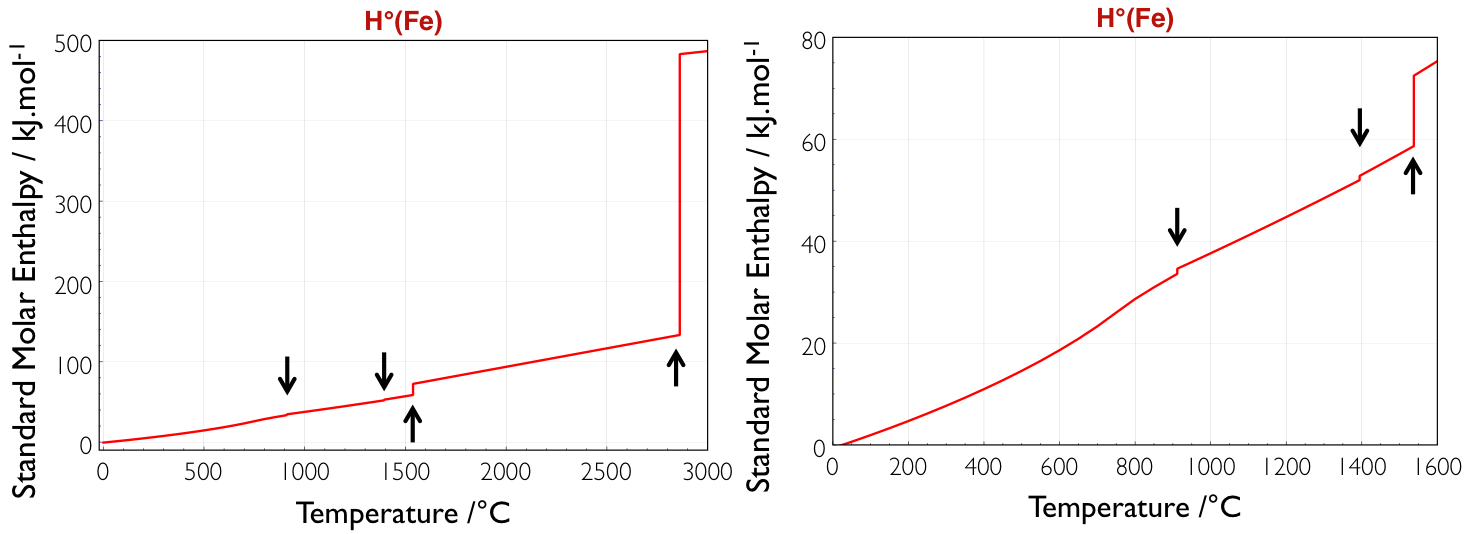
\includegraphics[width = \textwidth]{H_of_T_labeled.png}
\caption{$H\degree (T)$ for Fe over two temperature scales.}
\label{enthalpy_vs_T}
\end{figure}
The solid$\to$solid phase transitions' discontinuitites are barely visible on the left curve. This is because the latent heats of the different phase transitions differ by several orders of magnitude: $\Delta H_\text{Fe}^{\alpha \rightarrow \gamma} \approx 1$ kJ/mol and $\Delta H_\text{Fe}^{\gamma \rightarrow \delta} \approx 1$ kJ/mol. A large enthalpy for a solid$\to$solid phase transition is observed for zirconia's \href{http://en.wikipedia.org/wiki/Diffusionless_transformation#Martensitic_transformation}{martensitic phase transformation}, where $\Delta H_{\text{ZrO}_2}^{\text{tetra}\rightarrow \text{non}} \approx 6$ kJ/mol.  

The enthalpy of fusion (equivalently, the enthalpy of melting) is generally much higher. Richard's rule says that the enthalpy of fusion is proportional to the melting temperature of an element. 
%\begin{figure}[h]
%\centering
%\includegraphics[width = 12cm]{H_of_T_Fe_zoomed_out.png}
%\caption{The correlation between the enthalpy of melting and the melting temperature for the elements.}
%\end{figure}
%
\begin{equation}
\Delta H_\text{fusion} [\text{J/mol}] \approx 9 T_\text{fusion} [\text{K}]
\end{equation}
In most metals $\Delta H_\text{fusion}$ is on the order of 10 kJ/mol.  The elemental heat of vaporization follows a similar rule, Trouton's rule, which states that the the enthalpy of vaporization is proportional to the boiling temperature\footnote{As we will learn later, these rules imply that the entropies of melting and boiling are approximately equivalent for all of the elements}.
\begin{equation}
\Delta H_\text{vap} \approx 90 T_\text{vap}
\end{equation}
In most metals,  $\Delta H_\text{vap}$ is on the order of 100 kJ/mol.  The binding energies of metals are also on the order of 100 kJ/mol; you can intuitively think of evaporation as putting in the energy to break the bonds between atoms. We will emphasize understanding the orders-of-magnitude of energy scales in materials science throughout, sticking to engineering units of kJ/mol\footnote{Understanding in terms of atomic mechanisms is sometimes useful, wherein the natural units are eV/atom. $1 \text{ eV/atom}= 96.354\text{ kJ/mol}\approx 100\text{ kJ/mol}$. An especially good article on energy scales in materials science is  \href{http://dx.doi.org/10.1080/14786430500155080}{Spaepen, Phil. Mag. 2005}}.

\begin{figure}[h]
\centering
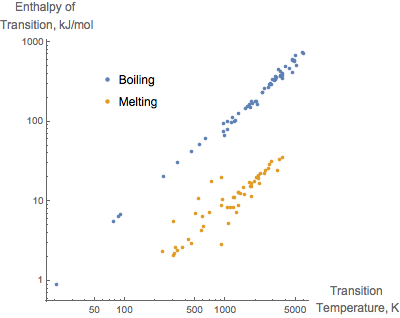
\includegraphics[width = 10cm]{Trouton_and_Richards_rules.png}
\caption{Elemental phase transition temperatures and enthalpies on a log-log scale. The slope of this correlation (on a linear scale) gives the characteristic entropy of these phase transitions. The correlation is stronger for boiling as compared to melting because the liquid$\to$gas transition's entropy change is dominated by the gain of translational degrees of freedom, whereas the gain in entropy upon melting can be appreciably changed by the local interactions in the solids and liquids of the elements. Positive deviations from Richard's rule occur for heavy semimetals: Sb, Bi, Sn, Te have larger entropies of melting than expected. Negative deviations occur for elements with unfilled f-orbitals: Pu, Ce, Nd have smaller entropies of melting than expected. Simple metals and transition metals are well-behaved.}
\label{Trouton_Richard}
\end{figure}

Now, what is the relative contribution of the $PdV$ term to these phase transition enthalpies?  We can estimate this by plugging in approximate numbers. We'll consider the case of two condensed phases, phase I $\rightarrow$ phase II.  In a metal, $V_{molar} \approx 10 \text{ cm}^3\text{/ mol}=10^{-5} \text{ m}^3\text{/ mol}$ and a good upper bound on the volume change is $\sim$ 10\% $\Delta V$.  At atmospheric pressure, P\degree = $10^5$ Pa, so $P \Delta V = 10^5 \cdot 10^{-6} = 0.1 \text{ J/mol}$. Note the use of J/mol instead of kJ/mol here: \emph{the energy scale associated with pressure-volume effects can only moderately perturb the energetics of condensed-matter phase transitions, except at very high pressures}.

Just as it is useful to understand the energy scales associated with P-V work, it is also useful for us to understand the energy scales associated with chemical reactions. In chemistry, this is characterized by the enthalpy of formation of molecules, in the solid state, the relevant quantity is the enthalpy of formation of compounds:\\

At room temperature and pressure:
%I am confused what you were trying to say here, any idea, Derek?
\begin{equation}
2 Fe_{(s)}^{\alpha} + \frac{3}{2}O_{2 (g)} \rightarrow Fe_2O_{3 (s)}^{\alpha} + (\Delta Q)_p
\end{equation}
with $(\Delta Q)_p$ = -1963 kcal/mol.  The sum enthalpy of the reaction $\Delta_v H$ is then:
\begin{equation}
\Delta_v H = \Delta H^0_{Fe_2O_3} - \Delta H^0_{Fe} - \frac{3}{2} \Delta H^0_{O_2}
\end{equation}
and, for reference, we have:
\begin{align*}
\Delta H^0_{Fe_2O_3} &= -820.5 \text{kJ}/\text{mol}\\
\Delta H^0_{Fe} &= 0\\
\Delta H^0_{O_2} &= 0\\
\Delta H^0_{CO} &= -110.52 \text{kJ}/\text{mol}\\
\Delta H^0_{CO_2} &= -393.51 \cdot \text{kJ}/\text{mol}
\end{align*}

There are plenty of references to get these values, such as \un{Janaf tables}.  Examples include FactSage \& Thermocalc and they provide $H^0$, $G^0$, $C_p^0$, etc.

\begin{align*}
C_{(s)} + O_{2 (g)} &\rightleftharpoons CO_{2 (g)}\\
\Delta_r H^0 &= -393.52 \text{kJ}/\text{mol}\\
C_{(s)} + \frac{1}{2} O_{2 (g)} &\rightleftharpoons CO_{(g)}\\
\Delta_r H^0 &= -110.52 \text{kJ}/\text{mol}\\
C_{(s)} + CO_{2 (g)} &\rightleftharpoons 2 CO_{(g)}\\
\Delta_r H^0 &= +183.00 \text{kJ}/\text{mol}\\
\end{align*}

The $\Delta H$ only tells you how much heat is exchanged, it doesn't tell you which reaction is \emph{going to happen}. Exothermic reactions release heat, which tells you that a given reaction is favorable in terms of its bonding. The first two reactions are exothermic; carbon and oxygen prefer to bond to one another. The last reaction is endothermic, meaning that the formation of $CO_{(g)}$ is not energetically favorable from  $CO_{2 (g)}$ and $C_{(s)}$. However, enthalpy is not the whole story in determining the spontaneity of reactions: energy conservation alone cannot tell you in which direction a reaction will occur.
%Be careful with the idea of ``heat'' content.  The fact that a reaction re't mean we're going to harvest this energy as heat. The first law is also silent about the directions of change $\rightleftharpoons$.  

%%%%%%%%%%%%%%%%%%%%%%%%%%%%%%%%%%%%%%%%%%%%%%%%%%%%%%%%
\section{Lecture - September 9, 2014}
% In previous lectures we worked with the first law with both the heat and work terms.  In continuation, imagine we have a lightbulb.  We can model the work as
% \begin{align*}
% W_\text{electric} = \partial Q + E_{\hbar v}
% \end{align*}
% If we have two compartments that are connected, one at $T_1$ and another at $T_2$ with $T_1 > T_2$ and $Q_1 < 0$ \& $Q_2 > 0$.
In previous lectures, we worked with the first law with both the heat and work terms.  In continuation, we examine how different processes can be modeled within this framework, and the importance of the proper definitions of systems and boundary conditions in obtaining the correct results. We do so by considering different processes that an ideal gas can undergo.

\bold{An aside on the ideal gas}:  The ideal gas is a convenient system to examine thermodynamically because its internal energy can be defined in terms of just one state variable, the temperature: $U = U(T)$. Specifically, the internal energy of an ideal gas is\footnote{We'll prove this in statistical mechanics, but it is proven from the ideal gas law \href{http://pruffle.mit.edu/3.00/Lecture_11_web/node1.html}{here}.}:
\begin{align*}
dU=C_V dT=(C_P-nR)dT\\
\Delta U=C_V \Delta T = (C_P-nR) \Delta T
\end{align*}
In addition, we also have a nice \emph{equation of state} to relate changes in the thermodynamic state variables to one another, the ideal gas law, $PV=nRT$.

\subsection{Throttling processes}

 Consider a bike tube initially at room temperature ($T=298K$) with $P=4.4$atm (50 psi).  Now, we release the pressure from the bike tire and let air out; the air exiting the tube undergoes what is called a \emph{throttling process}. We are interested in how the thermodynamic state of the gas will change as it is released, in particular, what will be the temperature of the air right outside the nozzle?\\

First, we define our system as the gas which is released. It undergoes a sufficiently rapid expansion that the process can be approximated as adiabatic (not enough time for system to exchange heat with its environment). Then:
\begin{align*}
dU_\text{gas} &= \delta Q + \delta W = \delta W \\
&= -P dV\\
&= n C_V dT = -P dV
\end{align*}
Note that $V = nR\frac{T}{P}$, taking the total differential of $V$:
$$
dV = \frac{n R}{P} dT - nRT \frac{dP}{P^2}
$$

% \begin{align*}
% V &= nR\frac{T}{P}\\
% dV &= \frac{n R}{P} dT - nRT \frac{dP}{P^2}
% \end{align*}

Plugging in this defintion of $dV$ above gives the final temperature in terms of the initial temperature and the ratio of the pressures:
\begin{align*}
nC_V dT &= -nRdT + RT \frac{dP}{P}\\
\Big(\frac{T_2}{T_1}\Big)^{C_P/ R} &= \frac{P_2}{P_1}\\
T_2 &= T_1 \Big(\frac{P_1}{P_2}\Big)^{R/C_P}
\end{align*}

For the bike tube, this gives $T_2 = 206$K = -67\degree C.  Why didn't we actually reach this temperature?  Well, the gas flowed through a nozzle instead of simply isotropically expanding, and the pressure outside the gas was not equal to the pressure inside the gas during the expansion. Clearly, we need to examine this process from a different perspective. Often, in thermodynamics, this means you need to re-define your system. We do so below.\\

\bold{What is happening through the valve?}  %\un{Joule-Thompson expansion} 
We now define our system as the valve. In this case, the system is at constant volume, and the key process taking place is that gas is flowing through the system. These gas molecules have some well-defined internal energy, so there is an energy flux through the system due to the mass flux through the system:
\begin{equation}
dU_\text{valve} = U_\text{in} d n - U_\text{out} d n + \delta Q
\end{equation}
The gas enters with $P_\text{in}$ and a specific volume $v_\text{in}$ then leaves with $P_\text{out}$ and $v_\text{out}$.  Even though the valve is a constant volume system, the mass flux implies that we will have a work term. The work done by the incoming gas is $P_\text{in} V_\text{in}$, the work done by the outgoing gas is $P_\text{out} V_\text{out}$. They have opposite signs due to the $dn$ term. $\delta Q$ is zero because the process is adiabatic, so:
\begin{equation}
dU_\text{valve} = \delta W = d n (P_\text{in} v_\text{in} - P_\text{out} v_\text{out})
\end{equation}
%The valve is an \un{open system} (can exchange particles with environment), and 
Equating these two definitions of $dU_\text{valve}$ gives:

$$
(U_\text{in} - U_\text{out}) = (P_\text{in} V_\text{in} - P_\text{out} V_\text{out})\footnote{This is a statement that the enthalpy of the gas during the throttling process is constant: $U_\text{in}+P_\text{in} V_\text{in}=U_\text{out}+P_\text{out} V_\text{out}$, so $H_\text{in}=H_\text{out}$. Note that this doesn't need the ideal gas asssumption, it's general.}
$$
Using the ideal gas equations:
$$
n C_V \Delta T = nR(\Delta T)
$$
This implies that either $C_V = R$, or $\boxed{\Delta T=0}$. It turns out that an ideal gas undergoing this process should have $\Delta T = 0$. 

Note how changing the way we interpet the process generally leads to a different answer. In this case, we needed to use an interpretation where the pressure on the gas during the expansion was not equal to its internal pressure. This means that the process is non-equilibrium and irreversible. This process is called a Joule-Thomson process. You can learn more about it on wikipedia, or refer to \bold{Callen pg. 95}.

In general, we categorize processes in the following way: 

\begin{enumerate}[(I)]
\item Continuous and at equilibrium with environment (reversible). See Figure 2.
\item Continuous but not necessarily at equilibrium with environment.  This is considered \un{quasi-static}.  Can be both reversible and irreversible.  See Figure 3.
\item Discontinuous and not in equilibrium.  We can not do equilibrium thermodynamics for this.  (i.e. an explosion with H\2 + O\2 will proceed so fast we can not tell what is happening to get us to the final stage.  See Figure 4.
\end{enumerate}

\subsection{Quasistatic Piston}
We now consider a piston slowly compressing a gas. See Callen Figure 5.
\begin{equation}
\sum_{i=1}^2 \frac{\dbar Q_i}{T} = \text{constant}
\end{equation}
Our path only depends on 1 (initial state) and 2 (final state).  The above is also our state function.\\

Let's assume that $dS = \frac{\dbar Q}{T}$.\\
\bold{Process 1}: Let's take a reservoir that is adiabatically isolated with $T_1$.  Let's transfer $\dbar Q$ to the reservoir.  The resulting temperature will then be $T_2$.\\
\bold{Process 2:} Now we have a propeller going into our reservoir with adiabatic walls and $T_1$.  Here, we have $dS_1 = dS_2 \neq \frac{\dbar Q}{T}$.\\

Second Law of Thermodynamics:  There exists a state function (property S) for which holds (closed system)
\begin{equation}
dS_\text{system} \geq \frac{\dbar Q}{T}
\end{equation}
it fixes the direction of change.  Forward ($1\rightarrow 2$) if $dS_f \geq \frac{\dbar Q_f}{T}$ or backward ($2\rightarrow 1$) if $dS_b \geq \frac{\dbar Q_b}{T}$.\\

If a process is \un{reversible} (quasi-static), then we have $dS = \frac{\dbar Q}{T}$.  If it is \un{irreversible}, $dS > \frac{\dbar Q}{T}$ (or $dS_\text{rev} + \xi$ where $\xi >0$).  The first law said that $U$ exists and
\begin{equation}
dU = \dbar Q + \sum y_i dx_i
\end{equation}
while the second law says $S$ exists and for a closed system
\begin{equation}
dS \geq \frac{\dbar Q}{T}
\end{equation}

Back to the example of two compartments that are connected (one at $T_1$ and the other at $T_2$), see Figure 6, we get
\begin{align*}
\dbar Q_1 &= -\dbar Q_2\\
dS_\text{system} &= dS_1 + dS_2\\
dS_\text{system} &= \frac{\dbar Q_1}{T_1} + \frac{\dbar Q_2}{T_2}\\
&= \frac{\dbar Q_1}{T_1} - \frac{\dbar Q_1}{T_2}\\
&= \dbar Q_1 (\frac{1}{T_1} - \frac{1}{T_2})\\
&= \dbar Q_1 (\frac{T_2 - T_1}{T_1 T_2}) \geq 0\\
\end{align*}
If $T_2 > T_1$, $\delta Q_1 > 0$.  Or if $T_2 < T_1$, then $\dbar Q_1 < 0$.  \textbf{Heat flows from ``hot'' to ``cold''}.

%%%%%%%%%%%%%%%%%%%%%%%%%%%%%%%%%%%%%%%%%%%%%%%%%%%%%%%
\section{Lecture - September 10, 2014}
As a reminder, the 1st law stated that $U$ is a state function where
\beq
dU = \dbar Q + \sum y_i dx_i
\ceq
The 2nd law states that $S$ is also a state function, and for a \emph{isolated system} under any arbitrary process,
\beq dS \geq \frac{\dbar Q}{T} \ceq
If the process is reversible then, $TdS = \dbar Q$.  The change in the entropy for the entire system must increase ($dS_\text{system} \geq 0$).
Key properties of entropy:
\begin{enumerate}[(I)]
\item $S$ of a system is \emph{not} a conserved quantity; entropy can be removed from a system, even during an irreversible process (This is what a refrigerator does, it irreversibly cools a system by increasing the entropy of the surroundings). 
\item $S$ of the \emph{universe} is only conserved during reversible processes. Otherwise, $S_\text{universe}$ is an increasing quantity (Imagine the case where we stir an isolated bucket with a propeller).
\item $S$ of an adiabatic system is constant or increases.  This is because the $\dbar Q$ term is zero, so $dS \geq 0$. %This seems redundant to me...
%\item $S$ \emph{can} decrease.  An example is allowing a liquid to cool and form a solid phase.  In this case the entropy of the system decreases.  The entropy of the environment, however, increases by an amount greater than or equal to the decrease of iron entropy.  Thus, $dS_\text{universe}$ is positive.
\end{enumerate}
\subsection{Consequences of the 2nd law:}
\begin{enumerate}[(I)]
\item \un{Irreversibility and `lost work'}: For processes with the same initial and final states, the work done by a system upon its surroundings during a reversible process is greater than or equal to the work done by a system during an irreversible process.
\beq \dbar W_\text{reversible} < \dbar W_\text{irreversible} \ceq
For a reversible path, \beq dU_\text{reversible} = \dbar Q_\text{reversible} + \dbar W_\text{reversible} \ceq
and the second law allows us to replace $\dbar Q_\text{reversible}$ by $TdS$.  For an irreversible path, U is a state function, so $dU$ is the same:

\beq dU_\text{reversible} = dU_\text{irreversible}  = \dbar Q_\text{irreversible} + \dbar W_\text{irreversible} \ceq
Since $T dS > \dbar Q_\text{irreversible} $ for an irreversible process, we have

\begin{align} T dS + \dbar W_\text{reversible} &= \dbar Q_\text{irreversible} + \dbar W_\text{irreversible}\\
T dS -\dbar Q_\text{irreversible}  &= \dbar W_\text{irreversible} - \dbar W_\text{reversible} > 0
\end{align}
so
\beq \boxed{\dbar W_\text{reversible} < \dbar W_\text{irreversible}}
\ceq
Note that our sign convention in these notes is $dU = \dbar Q + \dbar W$, so negative work is work done by the systems upon the surroundings. The important physical implication is that that if you want to extract work from a system, you get the most work out if the work is performed reversibly. Work that is not obtained from a process due to irreversibilities is sometimes called \emph{lost work}. Similarly, and perhaps more intuitively, if you want to do work upon a system, you will expend the least energy if the work is done reversibly: \\ \emph{The dissipation inherent in irreversible processes is bad for efficiency, regardless of whether work is done by a system, or work is performed upon system.} %\footnote{This has significant implications for the operation of batteries and the  materials production, wherein we are generally aiming to make things as reversible as possible}
\item \un{Limits to heat-work conversion}: 
Since a reversible process leads to the highest efficiencies, it is then logical to use a reversible process to set a limit on the amount of work that we can get from a heat source, i.e. by reversibly transfering heat from hot to cold. One can consider any process to do so, here we consider a non-specific process. The steps are worked out, but not explained. An animated explanation can be found on \href{https://www.khanacademy.org/science/physics/thermodynamics/v/efficiency-of-a-carnot-engine}{Khan Academy}\footnote{Sal Khan is an MIT alum!}, and a good written explanation is on \href{https://en.wikipedia.org/wiki/Carnot_cycle}{wikipedia}.
%\begin{align*}
%\Delta U = 0 &= Q + W\\
%\Delta S = \oint \frac{\dbar Q}{T}& = 0\\
%&= \frac{Q_H}{T_H}
%\end{align*}
\begin{align*}
\Delta S &= \oint \frac{\dbar Q}{T} = 0\\
\Delta S &= \frac{Q_H}{T_H} + \frac{Q_L}{T_L} = 0\\
Q_H &= \frac{-T_L}{T_H} Q_L
\end{align*}
\begin{align*}
\Delta U = 0 &= Q + W\\
Q_H + Q_L &= -W\\
Q_H - Q_H \frac{T_L}{T_H} &= -W\\
Q_H (1 - \frac{T_L}{T_H}) &= -W\\
\end{align*}
This gives us the Carnot efficiency $\eta = \frac{-W}{Q_H}$ and 
\beq 
\boxed{\eta_{\text{heat$\to$work}} = 1 - \frac{T_L}{T_H}}
\ceq
To give a sense of these efficiencies, with $T_H = 100^0$ C = 373 K and $T_L$ = 25\degree C = 298 K, $\eta \approx 20$\%. Significant gains in efficiency can be gained by going to higher temperatures: if $T_H$ = 550\degree C, $\eta \approx 63$\%.

We can also use work to move heat.  This process is also limited by the second law, but is characterized by a different efficiency. Moving heat from hot to cold is spontaneous, so we are usually concerned with how much heat we can move from cold to hot. When making something that is already warm warmer, we have a \un{heat pump} and when making something cold colder, we have a refrigerator (or an air conditioner). The logical way to characterize such an efficiency is the amount of heat moved per unit work used (this is often referred to as the ``coefficient of performance'', or COP of a heat pump). One can derive that:
\beq COP_\text{heat pump} = \frac{-Q_H}{W} = \frac{T_H}{T_H - T_L} \ceq
\beq COP_\text{refrigerator} = \frac{Q_L}{W} = \frac{T_L}{T_H - T_L} \ceq
With $T_H = 25$C and $T_C = 0$C, $COP_\text{refridgerator} = 11$.\footnote{This counterintuitively means that burning a fire is actually an extremely inefficient way to heat a home. You could get an order of magnitude more bang-for-your-Joule if you could convert that chemical energy to work, and use a heat pump!}

Note that in the above derivation, no reference was made to a specific mechanism: \emph{the Carnot limit applies any time heat is being converted to work}. One example of an exotic device that does this is a thermoelectric. One can apply some basic thermoelectric theory to show that thermoelectrics will never be as efficient as steam engines unless the thermoelectric figure of merit, $ZT$, increases by around an order of magnitude.\footnote{See \href{http://dx.doi.org/10.1038/nmat2361}{Nature Materials Vol 8 Feb 2009 ``An inconvenient truth about thermoelectrics''}}. This is not to say that thermoelectrics are a bad topic to research, but that one should not believe that they will replace a conventional heat engine for turning heat into energy, unless the given application prohibits the use of a heat engine.

\end{enumerate}



%\un{Practically}, we use a fluid for heat transfer.  We add heat $Q_H$ to water that turns into steam and runs a turbine generating work $W$.  We take some heat $Q_L$ away from the  steam (often called a working fluid), causing the steam to condense. The cold condensate at $T_L$ is then flowed it back to the heat source.  We can have inefficiencies turning the turbine, condensing the steam back into water, and we can increase efficiency by going to higher temperatures. These are excellent and practical materials problems to work on in energy. % I would like to do a recitation on steam engines in the future.

Now that we have an expression for a differential change in entropy, we can compute  entropy changes from arbitrary processes, $\Delta S_{\text{process}}$.  We know the temperature dependence of $S$:
\beq C_c = \frac{(\dbar Q)_c}{dT} \ceq
Where the subscript c is for ``constant path''. A reversible process along such a path must have:
\begin{align*}
T(dS)_c &= (\dbar Q)_c\\
\Big(\frac{\partial S}{\partial T}\Big)_c &= \frac{C_c}{T} \\
\Big(\frac{\partial S}{\partial T}\Big)_p &= \frac{C_p}{T}\\
\Big(\frac{\partial S}{\partial T}\Big)_v &= \frac{C_v}{T}\\
\end{align*}

Ultimately, because temperature has an absolute zero, entropy should also have some reference value when $T=0$ K.  How do we come up with a reference entropy $S$?  Nernst got the Nobel prize for it in 1920.

\subsection{The 3rd law}
\textbf{As the temperature approaches zero, the magnitude of the entropy change in any reversible process is zero.}

We can then fix the entropy of the elements at 0 K, in their \un{equilibrium} state, as being equal to zero.\footnote{We will show the physical meaning behind the third law during statistical mechanics. For now, we take it as a postulate.} \beq S_{0\text{K}}^\text{element} = 0 \ceq
Because entropy is a state function, the entropy along different paths must converge to the same value as a system is cooled to absolute zero; the curves must look like the right of Figure \ref{ThirdLawConsistency}. Because compounds can be reversibly formed from their constituent elements, the entropy of any compounds must also be zero at 0 K, as $\Delta S_\text{formation}=0$: $S^{AB}_\text{0K} = 0$. By extension, \emph{at equilibrium, the entropy of all materials at absolute zero is zero}. 
%\beq A + B \rightarrow AB \text{  (at 0K})\ceq
\begin{figure}[h]
\centering
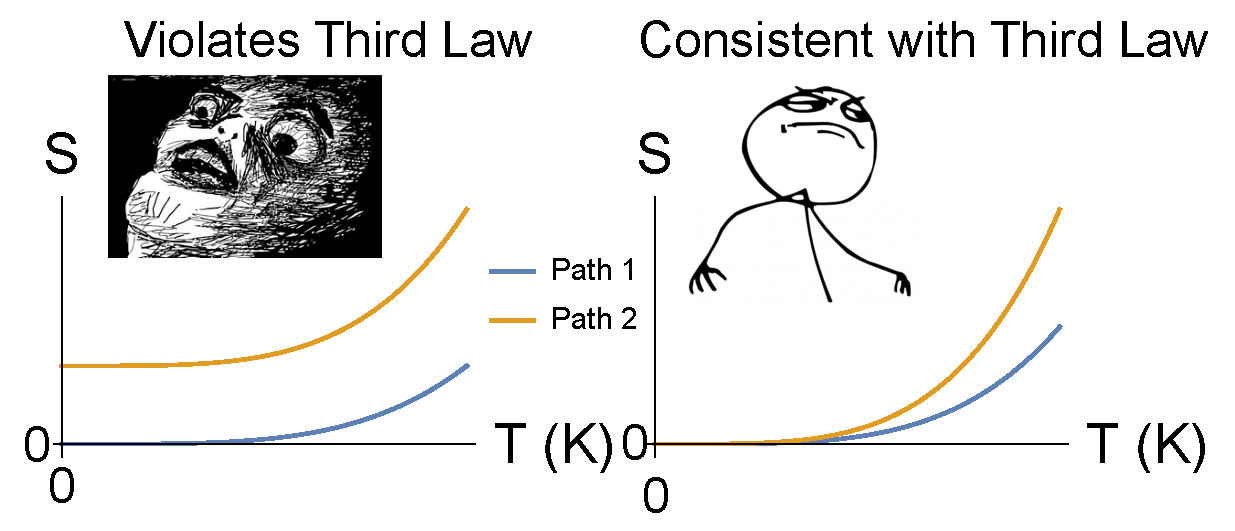
\includegraphics[width = 12cm]{thirdLawPlot_with_faces.pdf}
\caption{An illustration of entropy as a function of temperature inconsistent and consistent with the third law.}
\label{ThirdLawConsistency}
\end{figure}

%With this process $\Delta S = 0$ (reversible path) and .  Alternatively, it can be said that ``The entropy of a system at 0K is 0''.  This statement, however,is true if we are at \un{equilibrium}.

%Looking at the Entropy vs. Temperature handout, we see that the phase transformation at $\sim 900$\degree C results in a jump in both entropy and enthalpy.  $S$ is an extensive property and a state function.  For the $\alpha \rightarrow \gamma$ phase transformation
%\beq \Delta S_{\alpha \rightarrow \gamma} = \frac{\Delta H_{\alpha \rightarrow \gamma}}{T_{\phi T}} \ceq
%Say that we go from liquid to vapor, what is $\Delta S_{(l) \rightarrow (v)}$?  T $\approx$ 3000.\\

%\un{Trouton's rules}: $\Delta H_\text{vaporization} = 90 \times T_\text{vaporization}$.  With this, $\Delta S_\text{vaporization} \approx 90 \frac{J}{\text{mol} K}$.

\bold{Can we reach 0 K?}
\begin{figure}[h]
\centering
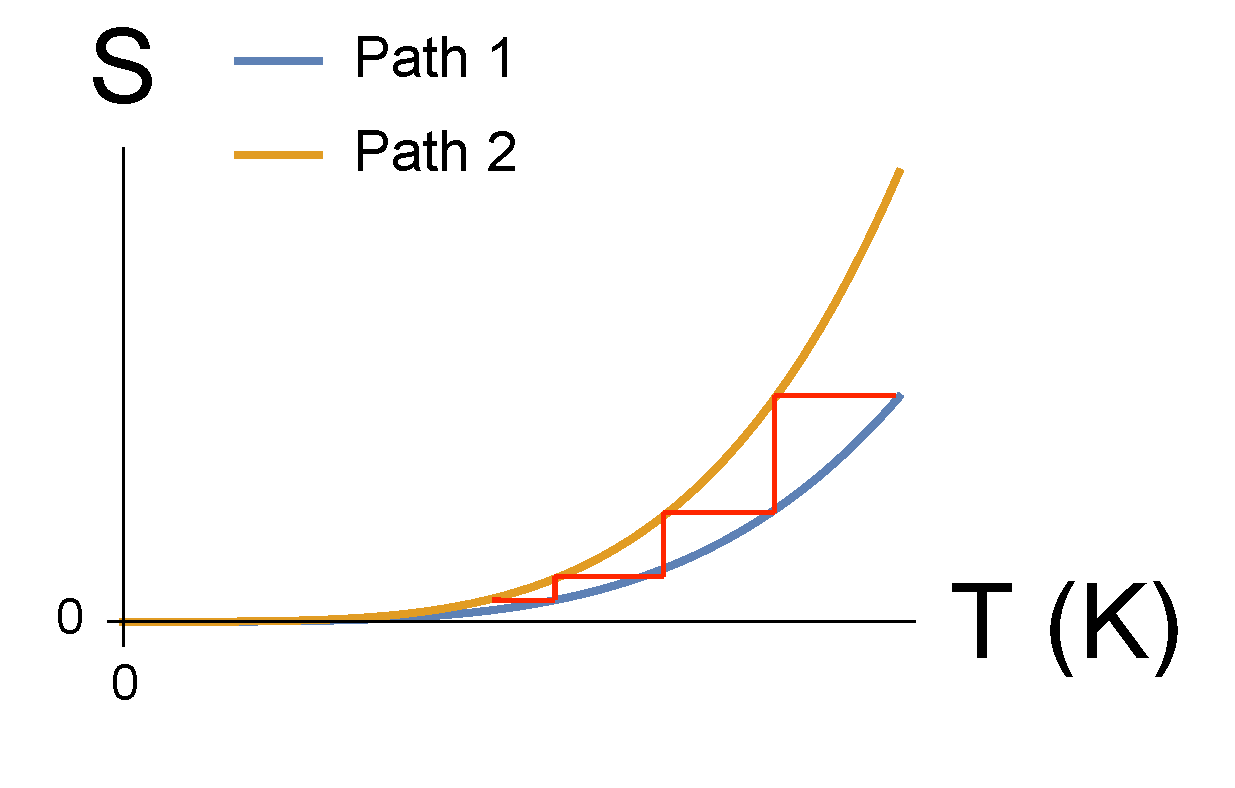
\includegraphics[width = 10cm]{Can_We_achieve_0K.pdf}
\caption{A T-S diagram illustrating the diminishing changes in temperature and entropy in a low-temperature, step-wise isothermal-isentropic cooling process. These changes become so small that an infinite steps are needed to reach 0 K.}
\label{Can_We_Reach_0_K}
\end{figure}

Consider trying to cool a material by extracting heat from the material and dumping it into a hotter reservoir. %$T_\text{outside}$ = 25\degree C and $T_\text{chamber} \approx  0.1$K.  
We would first need to extract the heat during a process when the material is in contact with the environment (say, through an isothermal compression), and then perform an adiabatic process on the material such that no heat flows in, and we are in a position to repeat the previous heat removal process (say, via an adiabatic expansion).  Of course, this would only work if you could make a series of heat reservoirs at lower and lower temperatures. See Figure \ref{Can_We_Reach_0_K}.  We can reduce the temperature by cycling between isothermal compression and isentropic (adiabatic) expansion, but we can never practically use this method to get to 0 K, as it would take an infinite number of cycles to do so. We can illustrate this by looking at the different processes individually:
\begin{enumerate}[(I)]
\item \un{Adiabatic expansion} of an ideal gas.  How much does the entropy change? You could try integrating the heat capacity along the path:
\beq T_2/T_1 = \frac{P_1}{P_2}^{R/C_v} \ceq
But that's kind of silly. You know that because it's adiabatic ($\dbar Q = 0$) then $d S = 0$.
\item \un{Isothermal} reversible expansion of an ideal gas.  $dS = \frac{\dbar Q}{T} = -\frac{\dbar W}{T} = \frac{PdV}{T} = nR \frac{dV}{V}$ (Know this since $U=U(T)$, and T constant means $\Delta U = 0 = Q + W$)

\beq 
\Delta S = nR\ln\Big(\frac{V_2}{V_1}\Big) 
\ceq
As volume goes up, entropy will too.
\item Arbitrary change of an ideal gas.  Since $S$ is a state function, we only need to find the reversible path.  We can break it up:
\beq dS = dS_\text{isobaric} + dS_\text{isothermal} = C_p \frac{dT}{T} - R\frac{dP}{P} \ceq

\end{enumerate}

%%%%%%%%%%%%%%%%%%%%%%%%%%%%%%%%%%%%%%%%%%%%%%%%%%%%%%%
\section{Lecture - September 12, 2014}
Now that the entropy has been defined, we are ready to start thinking about $U$ in terms of equilibrium processes, where we can replace $\dbar Q$ by $TdS$. In this case, an arbitrary change in the state of our system can be represented as:

\eqs
dU = TdS + \sum_i Y_i dX_i
\eqe
The above equation is sometimes called the \emph{combined first and second law}. It is also called the \emph{fundamental equation of physical chemistry}, because it is used to derive the rest of thermodynamics. Performing equilibrium thermodynamics in terms of $dU$ and its transformations is called the Legendre formulation of thermodynamics. One can equivalently formulate thermodynamics in terms of changes in the entropy of a system during arbitrary, reversible processes:
\eqs
dS = \frac{1}{T}dU +\frac{P}{T}dV - \sum_i \frac{\mu_i}{T}dN_i
\eqe
Energetic calculations are usually easier to do in the Legendre formulation, which is posed in terms of energy. The Massieu formulation is easier to use to think about the reversibility of processes, as it is posed in terms of entropy.

The combined first and second law leads to some powerful representations and insights into the properties of $U$.

\subsection{Mathematical Properties of $U$}
\subsubsection{U is first order homogeneous of the extensive variables, as is S}
The entropy is extensive (i.e. one can add the entropy of subsystems to obtain the entropy of a composite system). It also means that multiplying the size of the system by some parameter, $\lambda$, gives $\lambda$ times the original entropy: 
$S(\lambda U, \lambda X_i,...)=\lambda S(U,X_i,...)$

This states that the entropy is a first order homogeneous function. A similar argument can be made for the internal energy, which is also extensive. While one can make a somewhat hand-waving argument about integrating the internal energy to get a definition of $U$ instead of just $dU$, an elegant way to arrive at the same relationship is to make use of the fact that the internal energy is a first order homogeneous function. Hence, the purpose of discussing first order homogeneous functions is to avoid the physically murky reasoning that you need to introduce to integrate $dU$ to get $U$.

\subsubsection{U can be defined in terms of a sum of the conjugate pairs}
We derive this definition below. The result is sometimes called the \emph{Euler Relation}.

A general definition of an $n^\text{th}$ order homogeneous equation is:
$U(\lambda S, \lambda X,...)=\lambda^n U(S,X,...)$
We can take the derivative of both sides of this equation to get:
\eqs
\frac{\partial}{\partial \lambda} U(\lambda S,\lambda X,...) =n \lambda^{n-1} U(S,X,...)
\eqe
For n = 1, the right hand side is just $U(S,X,...)$. We can expand the LHS in terms of its derivatives with respect to the natural variables of U (the extensive variables):
\eqs
\frac{\partial (\lambda S)}{\partial \lambda} \frac{\partial U(\lambda S, \lambda X,...)}{\partial (\lambda S)} + \frac{\partial (\lambda X)}{\partial \lambda} \frac{\partial U(\lambda S, \lambda X,...)}{\partial (\lambda X)} + ... = U(S,X,...)
\eqe

It's pretty easy to see that $\frac{\partial (\lambda S)}{\partial \lambda} = S$, and $\frac{\partial (\lambda X)}{\partial \lambda} = X$, giving:
\eqs
S \frac{\partial U(\lambda S, \lambda X,...)}{\partial (\lambda S)} + X \frac{\partial U(\lambda S, \lambda X,...)}{\partial (\lambda X)} + ... = U(S,X,...)
\eqe

Now, this next part seems trivial, but it's actually a nice, subtle trick. We used the definition of a homogeneous first order function to get U on the right hand side, so anything on the left hand side is an alternative defintion of U. By setting $\lambda = 1$, we can set each of the remaining derivatives equal to the conjugate forces:
$\frac{\partial U(S, X,...)}{\partial S} = T$, $\frac{\partial U(S, X,...)}{\partial X} = Y$, and so on for all of the extensive variables.
Remembering that the right hand side is $U(S,X,...)$, this allows us to show that U is defined as:
\eqs
U(S,X,...) = TS + \sum_i Y_i X_i
\eqe

This definition is very useful, so it's important we have a rigorous basis for it (which we just showed above!). It gives us the Gibbs-Duhem equations, and also allows us to make changes of variables to other free energy functions which have different natural variables, such as the enthalpy, which has natural variables of $S$ and $P$:
\eqs H = U + PV \eqe
Plugging in the combined first and second law and the total differential of $PV$ gives:
\eqs dH = TdS +VdP \eqe
Note how the exact differential of $dH$ is naturally written in terms of new variables. We'll go in-depth into this type of transformation, a Legendre transform, and its implications in the next section.


%\[PartialD](\[Lambda]S)/\[PartialD]\[Lambda] \[PartialD]U(\[Lambda]S,\[Lambda]X,...)/\[PartialD](\[Lambda]S)+\[PartialD](\[Lambda]X)/\[PartialD]\[Lambda] \[PartialD]U(\[Lambda]S,\[Lambda]X,...)/\[PartialD](\[Lambda]X)+...=U(S,X,...)




% $U$ is a homogeneous function of first order in the \emph{extensive} variables; doubling the size of the system doubles all of the extensive variables (you double the volume, mole numbers, etc).
% \eqs
% f(\lambda x, \lambda ) = \lambda^r f(x,y)
% \eqe
% taking $r=1$ for $U$,
% \eqs
% f(\lambda x, \lambda y) = \lambda f(x,y)
% \eqe
% lets verify the result:
% \eqs
% \frac{\partial (U(\lambda S, \lambda X))}{\partial \lambda} &= \frac{\partial U}{\partial (\lambda S)} \frac{\partial (\lambda S)}{\partial \lambda} + \frac{\partial U}{\partial (\lambda X)} \frac{\partial (\lambda X)}{\partial \lambda}\\
% &= \frac{\partial U}{\partial (\lambda S)} S + \frac{\partial U}{\partial (\lambda X)}X\\
% &= \frac{\partial U}{\partial S} S + \frac{\partial U}{\partial X} X\\
% &= U(S,X)
% \eqe
% Thus for $\lambda = 1$
% \eqs
% U = TS + yx
% \eqe
\subsubsection{The Gibbs-Duhem equation: The intensive variables are not independent}
The Euler relation can give an independent definition of $dU$ by taking its total differential:
\eqs
d U(S,X,...) = T dS + S dT + \sum_i Y_i d X_i + \sum_i X_i d Y_i 
\eqe
Setting this equal to the definition of $dU$ from the combined first and second law gives:
\begin{align*}
TdS + \sum_i Y_i dX_i&=T dS + S dT + \sum_i Y_i d X_i + \sum_i X_i d Y_i \\
0 &=S dT + \sum_i X_i d Y_i
\end{align*} 

This is called a \emph{Gibbs-Duhem equation}. It states that all the intensive variables cannot be varied independently. They have a variety of convenient uses, and we will come back to them frequently in the last section of the class. An example of how a Gibbs-Duhem equation might be applied is as follows:\\

Let's think about how the chemical potential of a binary system changes. In particular, we'll consider the experimentally relevant case where the system is at constant pressure and temperature ($dP=dT=0$), and we are varying the chemical potential of one component (say by flowing a vapor with different concentrations through the system). Then, the Gibbs-Duhem equation simplifies to:
\eqs N_1 d \mu_1 = -N_2 d \mu_2 \eqe
In words, this says that varying the chemical potential of one component automatically causes the chemical potential of the other component to change in the opposite direction, and that the rate of this change is related to the mole numbers  of the two components in the system. This is a deep and unintuitive truth.

\subsubsection{Equations of state contain partial information about U}
Equations of state of $U$ are expressions of the intensive variables in terms of the independent variables. As a thermodynamic state is completely defined by the extensive variables alone, the equations of state provide the relation between the independent, extensive state variables and the dependent, intensive state variables. For example, $P\equiv (\partial U / \partial V)_{S,N_i}$, which implies that P is a function of the entropy and mole numbers at which the derivative was taken: $P = P(S,N,V)$. This expression, $P(S,N,V)$, is one equation of state for a simple system. The others are $T(S,V,N),\mu(S,V,N) $. As the equations of state are the derivates of the free energy, if you know enough of them, you can combine their integrals to get the free energy function as a function of its natural variables referenced to some initial state. For a system where the mole numbers are constant:
\eqs U(V,S)= \int_{V_0}^{V} \left(\frac{\partial U}{\partial V} \right)_{S_0} \,dV+\int_{S_0}^{S} \left( \frac{\partial U}{\partial S}\right)_{V}\,dS = \int_{V_0}^{V} P dV +\int_{S_0}^{S} TdS \eqe
However, such an integration can only be performed if you have as many independent equations of state as you have free variables, and you know them in terms of the proper variables (S and V in the case of U).



\subsection{Equilibrium and evolution of isolated systems}
We now use the Massieu formulation and the second law to derive the conditions of equilibrium for a variety of cases. The conclusion is: \emph{at equilibrium in an isolated, unconstrained system, the intensive variables are homogeneous (constant across the whole system)}. Below, we treat temperature, chemical potential, and pressure individually, but the results are general\footnote{This is similar to the discussion in Callen Chapter 4.4}.

%\subsubsection{An open and isolated system}
We consider a system where the possible work terms are exchange of energy, mole numbers, and volume. The chemical potential, $\mu$, is the intensive conjugate of $dN$ which is the change in number of particles.
\eqs
U &= TS - PV + \sum_i \mu_i N_i\\
dU &= SdT - VdP + N_i d\mu_i = 0
\eqe

For an isolated system, the 1st law says $U_\text{system}$ \& $ V_\text{system}$ are constant ($dV_\text{system}=dU_\text{system}=0$). The 2nd law says $dS_\text{system} \geq 0$.  S is maximized over the set of thermodynamic states that are consistent with the constraints on the extensive variables, i.e. the boundaries.  The equilibrium state is then the one with maximal S for our boundary conditions.\\

\subsubsection{Thermal Equilibrium}
Lets look at thermal equilibrium in a system with two containers I and II that allow energy to flow between them: $dU_I,dU_{II} \neq 0$.
\eqs
dU &= 0 = dU_I+dU_{II}\\
dU_I &= -dU_{II}\\
dS &= dS_I + dS_{II}\\
dS &= \frac{dU_I}{T_I} + \frac{dU_{II}}{T_{II}} \text{ (by Massieu/second law)}\\
dS &= dU_I \Big(\frac{1}{T_I}-\frac{1}{T_{II}}\Big)
\eqe
Now, if $T_I < T_{II}$ and $dU_I > 0$, then $dS > 0$ and we are \bold{not at equilibrium}.  If $T_I > T_{II}$ and $dU_I < 0$, then $dS > 0$ and we are also \bold{not at equilibrium}.  Equilibrium then occurs when $\frac{1}{T_I}-\frac{1}{T_{II}} = 0$, or $T_I = T_{II}$.

\subsubsection{Mechanical Equilibrium}
Consider two compartments of an isolated container separated by an diathermal, moveable wall.  The volume of the left side is $V_1$ and the right is $V_2$.
\eqs
dU_1 &= -dU_2\\
dV_1 &= -dV_2\\
dS &= dU_1 \Big(\frac{1}{T_1}-\frac{1}{T_{2}}\Big) + dV_1 \Big(\frac{P_1}{T_1}-\frac{P_2}{T_{2}}\Big)\\
\eqe
thus $S$ is maximal for $T_1 = T_2$ and $P_1 = P_2$.
\subsubsection{Chemical Equilibrium from Mass Flow}
Similarly, we can add a $\mu dN$ term to the energy change (or $-\frac{\mu}{T}dN$ in the entropy representation).  We then get an additional term to $dS$ of 
\eqs
dS = ... -\Big(\frac{\mu_1}{T_1}-\frac{\mu_2}{T_2}\Big)dN_1
\eqe
which results in equilibrium so long as $\frac{\mu_1}{T_1} = \frac{\mu_2}{T_2}$.  Enforcing thermal equilibrium means that $\mu_1=\mu_2$.  We can see from the signs of $dN_1$ and $dN_2$ that matter flows from high $\mu$ to lower $\mu$, as we would expect from a potential\footnote{In terms of kinetics, a gradient of $\frac{\mu}{T}$ generates mass flow (i.e. a diffusional relaxation toward equilibrium).}.

% \subsubsection{Chemical Equilibrium from Reactions}
% Given the reaction
% \eqs
% aA + bB \rightarrow cC + dD
% \eqe
In general, we can maximize the entropy by:
\begin{itemize}
\item defining the variables which are free to move in the system. For example: can subsystems exchange volume or mass? If so, $dV$ and $dN$ would be appropriate internal variables.
\item writing $dS$ as a function of the \emph{internal} variables in the Masseu formulation.
\item imposing $dS_\text{system} = 0$ for all the variations.
\end{itemize}
Thus, given appropriate internal variables, we can directly extract the equilibrium conditions.  For energy exchange, $dU_{1\rightarrow 2}$, we get $T_1 = T_2$.  For energy and volume exchange, $dU_{1\rightarrow 2}$ and $dV_{1\rightarrow 2}$, we have $T_1 = T_2$ and $P_1 = P_2$.  Another example would be charge exchange, $dq_{1\rightarrow 2}$, which implies a homogenous electrostatic potential: $\phi_1 = \phi_2$.


%% \subsection{Legendre Transforms}

%% We can perform a Legendre Transformation to come up with new representations of our system's energy
%% \eqs
%% dU = TdS + \sum_i y_i dx_i
%% \eqe
%% Lets consider a simple system.  We can write it in terms of several ``natural functions'' ($U(S,V)$ or $S(U,V)$)
%% \eqs
%% dU &= T dS - P dV\\
%% dS &= \frac{1}{T}dU + \frac{P}{T}dV
%% \eqe
%% also, we may integrate our function
%% \eqs
%% U(S,X_i) \rightarrow dU = \frac{\partial U}{\partial S}|_{X_i} dS + \frac{\partial U}{\partial X_j}|_{X_{i\neq j}} dX_j
%% \eqe
%% and thus we have relations for our equations of state
%% \eqs
%% T(S,X_i) &= \frac{\partial U}{\partial S}|_{X_i}\\
%% y_j(S,X_j) &= \frac{\partial U}{\partial X_j}|_{X_{i\neq j}} 
%% \eqe
%% If we just have one equation of state ($T(S,V)$), we can get
%% \eqs
%% U = \int dS T(S,V) + g_1(V)
%% \eqe
%% similarly if we only have $-P$
%% \eqs
%% U = -\int dV P(S,V) + g_2(S)
%% \eqe
%% The number of ways the system can exchange energy is equal to the number of equations of state (EOS).


%%%%%%%%%%%%%%%%%%%%%%%%%%%%%%%%%%%%%%%%%%%%%%%%%%%%%%%%%%%%%%%%%%%%%%%%%%%%%%%%%%%%%
%%%%%%%%%%%%%%%%%%%%%%%%%%%%%%%%%%%%%%%%%%%%%%%%%%%%%%%%%%%%%%%%%%%%%%%%%%%%%%%%%%%%%
\section{Lecture - September 15, 2014}


%\subsection{Equilibrium under the most general conditions}
%\textbf{Mike has not edited this section yet}
% We have extensive boundary conditions for an isolated system with a wall that allows the volume and internal energies of each side to change.   When the internal energy $U$ and position $x$ is a constant, the entropy is maximum.  When the entropy $S$ is constant then the internal energy is minimum.
% If we have an insulated, very large system, with temperature $T^*$ (where the $^*$ denotes the environment), and a smaller system within (no $^*$), and we assume that all variations are quasi-static, then
% \eqs
% \Delta U^* &= T^* \Delta S^* + \sum y_i^* \Delta x_i^*\\
% &= -\Delta U\\
% &= T^* \Delta S^* - \sum y_i^* \Delta x_i\\
% \Delta U - \sum y_i^* \Delta x_i &= -T^* \Delta S^*
% \eqe
% From the second law, we know that
% \eqs
% T^* (\Delta S* + \Delta S &\geq 0\\
% T^*\Delta S^* &\geq -T^*\Delta S\\
% -T^* \Delta S^* &\leq T^* \Delta S
% \eqe
% Therefore plugging into our previous result we have
% \eqs \boxed{
% \Delta U - \sum y_i^* \Delta x_i - T^* \Delta S \leq 0
% }
% \eqe
% In the above the $\Delta U$, $\Delta x_i$, and $\Delta S$ are the constraints for the \emph{system} and the $y_i^*$ and $T^*$ are the constraints for the \emph{environment}.\\

% \bold{Example:} A system interacting with the environment.  Consider a spring with mass $m$ hanging from it under the influence of gravity $g$.
% \eqs
% U_\text{sys} &= -mgx\\
% \vec{F} &= -k x
% dU_\text{sys} - T^* dS - F^* dx &\leq 0\\
% -mgdx - T^*dS + kx dx &\leq 0\\
% (kx - mg)dx \leq 0
% \eqe
% Thus we can tell $kx = mg$.

% \subsection{Assumptions}
% Lets begin to make some assumptions for a system
% \begin{itemize}
% \item The system will come to internal equilibrium with the environment (for a system + environment).
% \item No assumptions will be made about the \emph{internal state} of the \emph{system}
% \end{itemize}

% \un{For a simple system}
% \eqs
% dU - TdS + P dV \leq 0
% \eqe
% We can control the extensive variables for our system in the following ways
% \begin{itemize}
% \item \bold{Isolated}: $dU = 0$, $dV = 0$ which leads to $-TdS \leq 0 \rightarrow S_\text{max}$
% \item \bold{Adiabatic \& Isochoric}: $dS = 0$, $dV=0$ which leads to $dU \leq 0 \rightarrow U_\text{min}$
% \end{itemize}

\subsection{Legendre Transforms} \label{LegendreTransforms}
%$U$ is defubed a function of the extensive parameters $U(S,X,...)$. Frequently, we want a function $\phi(y)$ that is naturally a function of the intensive variables, raher than the extensive variables; it would be nice if we could specify the temperature instead of the entropy. 
The difficulty in working with the internal energy, $U$, is that it is a natural function of the wrong set of variables: V is the natural, `independent' variable of U for P-V work, whereas systems are usually kept at constant pressure, and S is the natural `independent' variable of U for reversible heat exchange\footnote{You can think of reversible heating as T-S work if you'd like.}, but systems are usually kept at constant temperature. What we seek is an alternative formulation of the internal energy which has the appropriate intensive variables as its natural, `independent' variables. \emph{Taking the Legendre transform is a general procedure to 'switch' which variables are the natural variables in your thermodynamic potential of interest.}\\

\textbf{How To Take a Legendre Transform}\\
If we want to transform U such that an intensive variable, $Y_i$, is the natural variable of the new, transformed potential, which we will call $\phi$, then we define $\phi$ as the difference of $U$ and the product $Y_i \cdot X_i$:
\eqs
\phi &= U - Y_i X_i\\
d\phi &= dU - Y_i dX_i - X_i dY_i
\eqe
where $dU = [...] + Y_j dX_j$.
Note that if U is composed of a sum of extensive variables times their intensives conjugates, $U=\sum_{j} Y_j X_j$, then $\phi=\sum_{j\neq i} Y_j X_j$. The total derivative of $\phi$ is then given by:
\eqs
d\phi &= \sum_{j\neq i} Y_j dX_j - X_i dY_i
\eqe
This has the desired property that $Y_i$ is a natural variable of $\phi$, $\phi = f(X_{j\neq i},Y_i)$.
Lets look at an example of an isobaric, isentropic ($dS=0$) system, considering the \bold{enthalpy}, $H$:
\eqs
dU &= TdS - PdV\\
H &= U + PV\\
dH &= dU + PdV + VdP\\
dH&= TdS + VdP\\
\eqe
and we can retrieve the following relations from $dH(S,P) = \Big(\frac{\partial H}{\partial S}\Big)_P dS + \Big(\frac{\partial H}{\partial P}\Big)_S dP$:
\eqs
T &= \Big(\frac{\partial H}{\partial S}\Big)_P\\
V &= \Big(\frac{\partial H}{\partial P}\Big)_S
\eqe\\

\textbf{Properties of Legendre Transforms}\\
\begin{enumerate}
\item $\Big(\frac{\partial \phi}{\partial Y_i}\Big)_{X_{i\neq j}}=-X_i$; the derivative of $\phi$ with respect to the appropriate intensive variable is minus its conjugate extensive variable.
\item $\phi$ has analogous extremal properties to U: Just as the equilibrium state when all of the extensive variables are set occurs when $U$ is minimal, so the equilibrium state for a given Legendre transform, $\phi$, occurs $\phi$ under the appropriate boundary conditions. For example, the equilibrium state at constant temperature and pressure is the state with minimal Gibbs free energy, the equilibrium state at constant entropy and pressure is the state with minimal enthalpy, etc. 
\item A corollary to (2) is that the choice of boundary conditions is arbitrary: each equilibrium state corresponds to a minimum in the appropriate free energy for the final set of state variables. To give a concrete example, if we take a system at constant temperature and pressure and allow it to equilibrate, the Gibbs free energy will be minimal. But, this equilibrium state will also have some well-defined volume and entropy at equilibrium. If, instead, we allowed a system to equilibrate at the volume and entropy which correspond to the equilibrium state from above (i.e. we minimize the internal energy for the analogous state), it will also have some temperature and pressure at equilibrium, and this T and P will correspond to the T and P that we originally minimized the Gibbs free energy for.
\item The pure double derivatives of $\phi$ are the negative inverse of the pure double derivatives of $U$. For example:
 \eqs \frac{\partial^2 U }{\partial V^2}_{S,N,...}&=-\frac{\partial P }{\partial V}_{S,N,...} &=(\beta_S V)^{-1}\\
 \frac{\partial^2 H }{\partial P^2}_{S,N,...} &=-\frac{\partial V }{\partial P}_{S,N,...} &=-\beta_S V \eqe
\end{enumerate}

\textbf{Why do Legendre transforms work? (Optional)}\\
The Legendre transform works because it is an effective switch of coordinate systems, and we don't lose any information in doing this switch of coordinates. This change of coordinates is possible because U is a convex function of the extensive variables, and because U is a `smooth' function of these variables (there are no discontinuities in the first derivative of U). Therefore, there is a one-to-one mapping between the first derivative of U with respect to the extensive variables and the extensive variable itself, as shown in the Figure \ref{LegendreGraph}\footnote{From \href{http://dx.doi.org/10.1119/1.3119512}{``Making sense of the Legendre transform'', RKP Zia et al. Am. J. Phys. 2007}, which is a really good read if you desire a deeper understanding of Legendre transforms.}:

\begin{figure}[h]
\centering
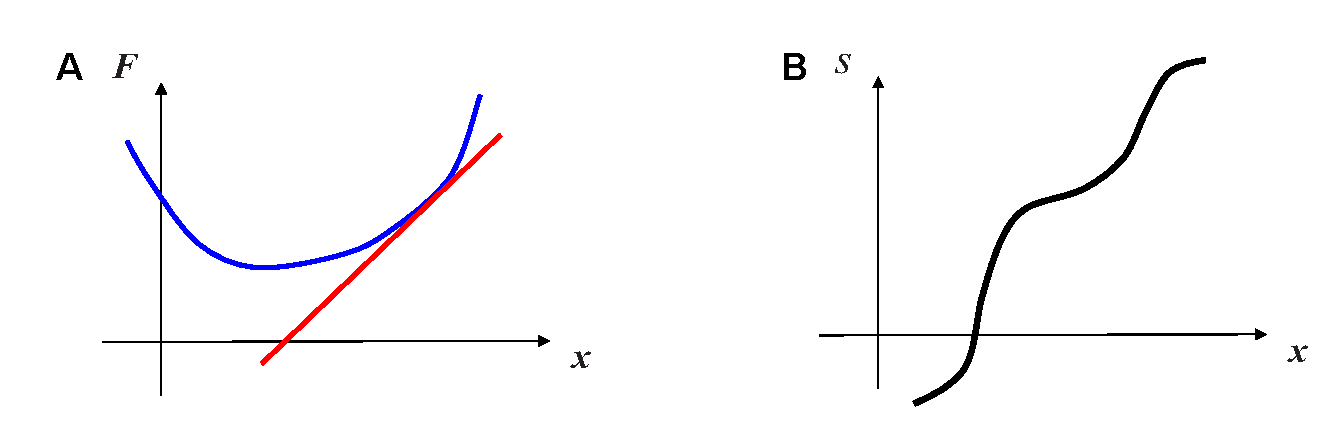
\includegraphics[width=\textwidth]{legendregraph.pdf}
\caption{\textbf{A} The graph of a convex function F(x). The tangent line at one point is illustrated. \textbf{B} The graph of $S(x)$, the slope of a convex function.}
\label{LegendreGraph}
\end{figure}

The one-to-one mapping of the slope of U with respect to its extensive variables and the extensive variables themselves means we can construct a new function from U that has the slope as its natural variable with no loss of information;  all the original thermodynamic information contained in U is also contained in its Legendre transforms, although in a different form. %The true convenience is that it still has units of energy, and that it has intuitive changes in concavity.


%%%%%%%%%%%%%
\subsection{Named Free Energies}
There are several other common Legendre transforms which have names. It would be wise to memorize these. The \bold{Helmholtz Free Energy} is:
\eqs
F &= U - TS\\
dF &= -SdT - P dV
\eqe
If we have a system where the temperature and volume are set experimentally, it makes sense to consider $F(T,V)$ since we will only need to minimize $F$ ($dF \leq 0$, $dV = 0$, $dT=0$).\\  
Similarly, the \bold{Gibb's Free Energy} is:
\eqs
G &= U-TS+PV\\
dG &= -SdT +VdP
\eqe
and we will have $dG \leq 0$ for a system where the temperature and pressure are set experimentally.  


% Put in a table of the free energy names
\begin{table}[ht]
  \centering
  %\Large
\caption{Some thermodynamic potentials for simple systems}
\renewcommand{\arraystretch}{1.5}% Spread rows out...
$\begin{array}{>{\centering\bfseries}m{1.8in} >{\centering}m{1.8in} >{\centering}m{1in} >{\centering\arraybackslash}m{1.4in}}
\toprule
\hline %inserts double horizontal lines
\textbf{T.D. potential} & \textbf{Differential} & \textbf{Natural variables} & \textbf{ Maxwell's}\\[2ex] 
\hline  % inserts single horizontal line
U & $dU=T\cdot dS -P \cdot dV$ & U(S,V) &  $(\frac{\partial{T}}{\partial{V}})_{S}=-(\frac{\partial{P}}{\partial{S}})_{V}$ \\[2ex]
F=U-TS & $dF=-S\cdot dT-P \cdot dV$ & F(T,V) & $(\frac{\partial{S}}{\partial{V}})_{T}=(\frac{\partial{P}}{\partial{T}})_{V}$\\[2ex]
H=U+PV & $dH=T\cdot dS+V \cdot dP$ & H(S,P) & $(\frac{\partial{T}}{\partial{P}})_{S}=(\frac{\partial{V}}{\partial{S}})_{P}$\\[2ex]
G=U-TS+PV=H-TS & $dG=-S\cdot dT+V \cdot dP$ & G(T,P) & $-(\frac{\partial{S}}{\partial{P}})_{T}=(\frac{\partial{V}}{\partial{T}})_{P}$\\[2ex]
%$\Phi_G$=U-TS-$\mu$N & $d\Phi =-S \cdot dT-P \cdot dV-\mu \cdot dN$ &  $\Phi_G(T,P)$ & \\[2ex]
\bottomrule
\end{array}$
\end{table}

\subsection{A First Look at Manipulating Thermodynamic Functions}
Lets now look at a simple system using the Gibb's free energy $G(T,P)$.  First, we know from the above that $S = -\Big(\frac{\partial G}{\partial T}\Big)_P$ and $V = \Big(\frac{\partial G}{\partial P}\Big)_T$.  The change in volume is
\eqs
dV &= \Big(\frac{\partial V}{\partial T}\Big)_P dT + \Big(\frac{\partial V}{\partial P}\Big)_T dP\\
&= \alpha_V V dT - V \beta_T dP
\eqe
since $\alpha_v = \frac{1}{V} \frac{\partial V}{\partial T}|_P$ is the volumetric thermal expansion and $\beta_T = -\frac{1}{V}\frac{\partial V}{\partial P}|_T$ is the compressibility.  Likewise, the change in entropy is
\eqs
dS &= \Big(\frac{\partial S}{\partial T}\Big)_P dT + \Big(\frac{\partial S}{\partial P}\Big)_T dP\\
&= \frac{c_P}{T}dT + \Big(\frac{\partial S}{\partial P}\Big)_T dP
\eqe
It's not really obvious what $\frac{\partial S}{\partial P}|_T$ is. We can use a \bold{Maxwell Relation} to gain some insight.  For this, we note that the second derivative of a function does not depend upon the order in which the derivatives are exchanged.
\eqs
\frac{\partial}{\partial P}\left(\left(\frac{\partial G}{\partial T}\right)_P\right)_T &= \frac{\partial}{\partial T}\left(\left(\frac{\partial G}{\partial P}\right)_T\right)_P\\
\frac{\partial}{\partial P}(-S)_T &= \frac{\partial}{\partial T}(V)_P\\
-\left(\frac{\partial S}{\partial P}\right)_T &= \left(\frac{\partial V}{\partial T}\right)_P = \alpha_V V\\
\eqe
and from here we can make our substitution into the above
\eqs
dS &= \frac{c_P}{T}dT - \alpha_V V dP
\eqe
This might seem a bit strange. The change in entropy with respect to pressure at a constant temperature is equal to minus the thermal expansion coefficient. This is not intuitive, but it pops right out of the mathematical structure of thermodynamics. Maxwell relations can be useful in this way, as they allow us to express difficult-to-measure quantities in terms of easily measurable experimental quantities. Further, they allow us to reason about the sign of quantities which we might not otherwise have much intuition about.  We can now say with certainty that except in cases where the thermal expansion coefficient is negative, the entropy of a substance decreases when you compress it\footnote{You can think of this heuristically as being true because the number of microstates becomes smaller as you confine a group of particles to a smaller space.}.
%%%%%%%%%%%%%%%%%%%%%%%%%%%%%%%%%%%%%%%%%%%%%%%%%%%%%%%%%%%%%%%%%%%%%%%%%%%%%%%%%%%%%%%%%%%%%%%%%%%%%%%%%%%%%%%%
%%%%%%%%%%%%%%%%%%%%%%%%%%%%%%%%%%%%%%%%%%%%%%%%%%%%%%%%%%%%%%%%%%%%%%%%%%%%%%%%%%%%%%%%%%%%%%%%%%%%%%%%%%%%%%%%
\section{Lecture - September 17, 2014}
\subsection{Maxwell Relations}
Previously we discussed \bold{Maxwell relations}, which allow us to swap a derivative in terms of some thermodynamic variables $x$ and $y$ for a derivative in terms of the conjugates of $x$ and $y$. They may be defined generally as
\eqs \boxed{
\left(\frac{\partial x}{\partial y}\right)_{\text{conj}[x]} = \pm \left(\frac{\partial {\text{conj}[y]}}{\partial {\text{conj}[x]}}\right)_{y}}
\eqe
The $ \pm $ in the above expression happens because the sign flips whenever you take a Legendre transform. The general procedure to create a Maxwell relation is then to: 
\begin{enumerate}
\item Legendre transform your potential so that the natural variables of the free energy are the variables you want in the denominator of the expression.
\item Equate the double partial derivatives.
\end{enumerate}
We now review some applications of Maxwell relations. 
\subsubsection{Maxwell relations for an Ideal Gas}
In general, $dS = \frac{c_P}{T}dT - \alpha_V V dP$. However, we can apply this in the case of an ideal gas to get a concrete expression for the change in entropy under changes in temperature and pressure:%, we saw that $-\frac{\partial S}{\partial P}|_T = \frac{\partial V}{\partial T}|_P$ and
\eqs
d(PV) = nR dT &= V dP +P dV\\
\Big(\frac{\partial V}{\partial T}\Big)_P &= \frac{nR}{P}
\eqe
Substituting gives: 
\eqs
\boxed{dS = -nR \frac{dP}{P} + c_P \frac{dT}{T}}
\eqe

\subsubsection{Magnetic Maxwell relations}
One can perform Maxwell relations including other work terms too. We demonstrate this here. In particular, let's say we wanted expressions relating the behavior of entropy in a magnetic field to other quantities that are more easily measured, say $\left(\frac{\partial S}{\partial P}\right)_{T,H}$ and $\left(\frac{\partial S}{\partial H}\right)_{T,P}$. Including magnetic work terms, $dU$ can be expressed as:
\eqs
dU = TdS - PdV + \mu_0 H_0 dM
\eqe
Here we have $U(S,V,M)$, but we need a thermodynamic potential expressed as a natural function of $T, P, H$ to perform the desired Maxwell relations, i.e. we want $\phi (T,P,H)$.  First, we perform a Legendre Transform:
\eqs
\phi &= U-TS + PV - \mu_0 H_0 M\\
d\phi &= -S dT + VdP - \mu_0 M dH\\
\eqe
This permits us to obtain the following relationships:
\eqs
\left(\frac{\partial S}{\partial P}\right)_{T,H} &= -\left(\frac{\partial V}{\partial T}\right)_{P,H} \\
\left(\frac{\partial (\mu_0 M)}{\partial T}\right)_{H,P} &= \left(\frac{\partial S}{\partial H}\right)_{T,P}  
\eqe

%%%%%
\subsection{How to perform thermodynamic derivations} \label{howToDerive}
We first give some general relationships from calculus that are useful in manipulating thermodynamic variables, and then we give you a general way to think about deriving quantities in thermodynamics.
\subsubsection{Very useful relationships of $f(x,y)$}
\textbf{Inverse rule}:
\eqs
\left(\frac{\partial f}{\partial x}\right)_y = \frac{1}{\left(\frac{\partial x}{\partial f}\right)_y}
\eqe
This relation is useful for getting things to the numerator from the denominator. This relationship only holds for well-behaved functions, but luckily thermodynamic functions are well-behaved.

\textbf{Chain rule}:
\eqs
\label{chainRule}
\left(\frac{\partial f}{\partial x}\right)_y = \left(\frac{\partial f}{\partial u}\right)_y \left(\frac{\partial u}{\partial x}\right)_y
\eqe
This is good if you can't take a derivative of f with respect to X, but you can take the derivative of u with respect to X (and hopefully of f with respect to u).


\textbf{Triplet rule}:
\eqs
\Big(\frac{\partial f}{\partial x}\Big)_y \Big(\frac{\partial x}{\partial y}\Big)_f \Big(\frac{\partial y}{\partial f}\Big)_x = -1
\eqe
This is good for changing paths: you get to hold different variables constant when taking the other two derivatves

\textbf{Another, unnamed rule} (Mike calls it the generalized chain rule):
%\eqs
%\label{genChainRule}
%\left(\frac{\partial f}{\partial x}\right)_y = \left(\frac{\partial f}{\partial u}\right)_y \left(\frac{\partial u}{\partial x}\right)_y
%\eqe
\eqs
\label{genChainRule}
\left(\frac{\partial f}{\partial x}\right)_g &= \left(\frac{\partial f}{\partial x}\right)_y + \left(\frac{\partial f}{\partial y}\right)_x \cdot \left(\frac{\partial y}{\partial x}\right)_g
\eqe
This is also good for changing paths, especially for heat capacity paths (this was the relation we used to derive the relationship between $C_p$ and $C_V$).
%%%%%
\subsubsection{Strategy to reduce variables}
Thermodynamic derivations are usually all about simplifying messy derivatives. The object of these derivations is to simplify them by substituting in known materials parameters. Hence, these guidelines are all about how to manipulate the derivatives so that you can start to substitute in known materials parameters.
\begin{enumerate}[(1)]
\item \un{Bring the thermodynamic potentials to the numerator.}\\
i.e. given  Joule-Thompson expansion (isenthalpic), we can remove the constraint of a derivative at constant enthalpy (which we don't know how to take) by using the triplet rule:
\eqs
\Big(\frac{\partial T}{\partial P}\Big)_H = -\frac{\Big(\frac{\partial H}{\partial P}\Big)_T}{\Big(\frac{\partial H}{\partial T}\Big)_P}
\eqe
\item \un{Always bring $S$ to the numerator and turn it into a heat capacity.}\\
i.e. from $dH = TdS + VdP$:
\eqs
\left(\frac{\partial H}{\partial P}\right)_T &= T \Big(\frac{\partial S}{\partial P}\Big)_T + V\\
\left(\frac{\partial H}{\partial T}\right)_P &= T \left(\frac{\partial S}{\partial T}\right)_P\\
\left(\frac{\partial T}{\partial P}\right)_H &= \frac{-(T \left(\frac{\partial S}{\partial P}\right)_T + V)}{T \left(\frac{\partial S}{\partial T}\right)_P}\\
&= \frac{-(T \left(\frac{\partial S}{\partial P}\right)_T + V)}{c_P}\\
&= \frac{-(-T\alpha_V V  + V)}{c_P}\\
&= \frac{V(T\alpha_V -1)}{c_P}
\eqe
(where the above used the Maxwell relationship $\left(\frac{\partial S}{\partial P}\right)_T = -\left(\frac{\partial V}{\partial T}\right)_P = -\alpha_V V$, and for an ideal gas we would have $\alpha_V = T^{-1}$, resulting in $\left(\frac{\partial T}{\partial P}\right)_H  = 0$)
\item \un{If needed, bring the volume to the numerator and turn it into a derivative of (T,P).}
\item \un{Relate heat capacities to what you know.}
\eqs
c_P - c_V &= T[\left(\frac{\partial S}{\partial T}\right)_P - \left(\frac{\partial S}{\partial T}\right)_V]\\
&= T[\left(\frac{\partial S}{\partial V}\right)_T \cdot \left(\frac{\partial V}{\partial T}\right)_P]
\eqe
In the above I used the relation
\eqs
\left(\frac{\partial f}{\partial x}\right)_g &= \left(\frac{\partial f}{\partial x}\right)_y + \left(\frac{\partial f}{\partial y}\right)_x \cdot \left(\frac{\partial y}{\partial x}\right)_g
\eqe
continuing, we have
\eqs
c_P - c_V &= T\left[\left(\frac{\partial S}{\partial P}\right)_T \cdot \left(\frac{\partial P}{\partial V}\right)_T \cdot \left( \frac{\partial V}{\partial T}\right)_P\right]\\
&= T\left[\left(\frac{\partial S}{\partial P}\right)_T \cdot \left(\frac{-1}{V\beta_T}\right) \cdot \left(\frac{\partial V}{\partial T}\right)_P\right]\\
\eqe
and from the Maxwell relation, $\left(\frac{\partial S}{\partial P}\right)_T = -\left(\frac{\partial V}{\partial T}\right)_P = -\alpha_V V$:
\eqs
c_P - c_V &= T\left[\frac{-\alpha_V V}{-\beta_T V} \alpha_V V\right]\\
&=\boxed{ T V \left(\frac{\alpha_V^2}{\beta_T}\right)}
\eqe
\end{enumerate}

%%%%%
\subsubsection{Example: A rod under tension}
Consider a rod that doesn't change volume and evolves adiabatically.  We apply a force $F$ to each end of the rod and obtain a change in pressure $dP$ as a result.  What happens to the temperature?
\eqs
dS &= \left(\frac{\partial S}{\partial T}\right)_F dT + \left(\frac{\partial S}{\partial F}\right)_T dF\\
dU &= TdS + Fdl
\eqe
From the triplet rule, $\left(\frac{\partial T}{\partial F}\right)_S \left(\frac{\partial F}{\partial S}\right)_T \left(\frac{\partial S}{\partial T}\right)_F = -1$, and thus
\eqs
\left(\frac{\partial T}{\partial F}\right)_S &= -\frac{\left(\frac{\partial S}{\partial F}\right)_T}{\left(\frac{\partial S}{\partial T}\right)_F}\\
&=-\frac{\left(\frac{\partial S}{\partial F}\right)_T}{\frac{c_F}{T}}\\
\eqe
Now what is $\left(\frac{\partial S}{\partial F}\right)_T$?  We can define a new potential
\eqs
\phi &= U - TS - Fl\\
d\phi &= -SdT - ldF
\eqe
which yields
\eqs
\left(\frac{\partial S}{\partial F}\right)_T = \left(\frac{\partial l}{\partial T}\right)_F = \alpha_L
\eqe
The thermal expansion coefficient $\alpha_L = \frac{1}{l} \left(\frac{\partial l}{\partial T}\right)_F$.  Putting this all together,
\eqs\boxed{\left(\frac{\partial T}{\partial F}\right)_S = - T l \left(\frac{\alpha_L}{c_F}\right)}
\eqe
Now all we need is the materials parameters.  $c_F \approx c_P \approx 25$ J/molK and $\alpha_L \approx 2 \cdot 10^{-5}$ 1/K, $\Delta (F/A) \approx 100 MPa$:
\eqs
\Delta T = -\left(\Delta \frac{F}{A}\right) (A \cdot l) T \frac{\alpha_L}{c_F}
\eqe
This results in a value of $\Delta T = -0.1 $K.  

%%%%%
\subsection{Natural Variables}
A question we may ask after all of this is: ``What are the natural variables for $U(S,V)$?'' Can we write $U(T,P)$? If so, what are the consequences?
\eqs
dU = \left(\frac{\partial U}{\partial T}\right)_P dT + \left(\frac{\partial U}{\partial P}\right)_T dP
\eqe
now let's take partials of the $U(S,V)$ we already know:
\eqs
\left(\frac{\partial U}{\partial P}\right)_T &= T\left(\frac{\partial S}{\partial P}\right)_T - P \left(\frac{\partial V}{\partial P}\right)_T\\
&= -T (\alpha_V V) - P (-\beta_T V)\\
&= V(P \beta_T - T\alpha_V)
\eqe
Similarly,
\eqs
\left(\frac{\partial U}{\partial T}\right)_P &= T\left(\frac{\partial S}{\partial T}\right)_P - P \left(\frac{\partial V}{\partial T}\right)_P\\
&= n c_P - P V \alpha_V
\eqe
and thus we can write
\eqs
dU = (n c_P - PV \alpha_V)dT + V(P \beta_T - T \alpha_V)dP
\eqe
Clearly, it is possible to think about $dU$ in terms of variations in the intensive variables, but it's much more natural to think of $dU$ in terms of $dV$ and $dS$.
\subsection{A systematic way to think about derivatives} \label{systematicWayDerivatives}
We're starting to build up a large number of derivatives and second derivatives of the free energies, it would be nice to have systematic way of representing and thinking of these derivatives. It turns out you can represent these derivatives as matrices. Lets look at the order of some derivatives of $G(T,P) \rightarrow dG = -S dT + V dP$:
\eqs
\left(\frac{\partial G}{\partial T}\right)_P &= -S\\
\left(\frac{\partial G}{\partial P}\right)_T &= V\\
\left(\frac{\partial^2 G}{\partial T^2}\right)_P &= -\frac{c_P}{T}\\
\left(\frac{\partial^2 G}{\partial P^2}\right)_T &= -\beta_T V\\
\eqe
We can display the order of derivatives as follows:\\
\begin{center}
\begin{tabular}{c | c | c}
 $G$ & $\frac{\partial}{\partial T}$ & $\frac{\partial}{\partial P}$\\ \hline
 $\frac{\partial}{\partial T}$ & $-\frac{c_P}{T}$ & $\alpha_V V$\\ \hline
 $\frac{\partial}{\partial P}$ & $\alpha_V V$ & $-\beta_T V$
\end{tabular}
\end{center}
If we add a \emph{magnetic field} our energy becomes $dU = TdS - PdV + H dM$.  The various derivatives of $\phi = U - ST + PV - HM$ result in the following order of (second) derivatives:
\begin{center}
\begin{tabular}{c | c | c | c}
$\phi$ & $\frac{\partial}{\partial T}$ & $\frac{\partial}{\partial P}$& $\frac{\partial}{\partial H}$\\ \hline
$\frac{\partial}{\partial T}$ & $-\frac{c_P}{T}$ & $\alpha_V \cdot V$ & $-\frac{\partial M}{\partial T}$\\ \hline
$\frac{\partial}{\partial P}$ & $\alpha_V \cdot V$ & $-\beta_T \cdot V$ & $V \cdot \gamma$\\ \hline
$\frac{\partial}{\partial H}$ & $-\frac{\partial M}{\partial T}$ & $V \cdot \gamma$ & $-V \cdot \chi$
\end{tabular}
\end{center}
You can write a similar matrix for any thermodynamic potential you choose. All such matrices are symmetric because of the Maxwell relations. The signs of the off-diagonal terms are a result of the Legendre transforms needed to get to the potential of interest. The signs of the diagonal terms are positive if the thermodynamic variable of interest is extensive, and negative if the variable of interest is intensive. This is because of the properties of the Legendre transform, and ultimately because $U$ is convex up with respect to the extensive variables.
%%%%%%%%%%%%%%%%%%%%%%%%%%%%%%%%%%%%%%%%%%%%%%%%%%%%%%%%%%%%%%%%%%%%%%%%%%%%%%%%%%%%%%%%%%%%%%%%%%%%%%%%%%%%%%%%%%%%%%%%%%%%%%%%%%%%%%%%%%%%%%%%%%%%%%%%%%%%%%%%%%%%%%%%%%%%%%%%%%%%%%%%%%%%%%%%%%%%%%%%%%%%%%%%%%%%%%%%%%%%
%%%%%%%%%%%%%%%%%%%%%%%%%%%%%%%%%%%%%%%%%%%%%%%%%%%%%%%%%%%%%%%%%%%%%%%%%%%%%%%%%%%%%%%%%%%%%%%%%%%%%%%%%%%%%%%%%%%%%%%%%%%%%%%%%%%%%%%%%%%%%%%%%%%%%%%%%%%%%%%%%%%%%%%%%%%%%%%%%%%%%%%%%%%%%%%%%%%%%%%%%%%%%%%%%%%%%%%%%%%%
\section{Lecture - September 24, 2014}
Last lecture we started to look at the difference the choice of path makes in measuring thermodynamic quantities. So, we asked ourselves the following: what is the relationship between the change in volume with respect to temperature at constant magnetization and its derivative at constant magnetic field? %($\frac{\partial V}{\partial T}|_M$)
\eqs
\left(\frac{\partial V}{\partial T}\right)_M \to? \left(\frac{\partial V}{\partial T}\right)_H
\eqe
We can apply the generalized chain rule, Eq. \ref{genChainRule}, in this situation:
\eqs
\frac{1}{V}\left(\frac{\partial V}{\partial T}\right)_M &= \frac{1}{V}\left(\frac{\partial V}{\partial T}\right)_H + \frac{1}{V}\left(\frac{\partial V}{\partial M}\right)_T \left(\frac{\partial M}{\partial T}\right)_H\\
&= \frac{1}{V}\left(\frac{\partial V}{\partial T}\right)_H + \frac{1}{V}\left(\frac{\partial V}{\partial M}\right)_T M'(T)\\
\eqe
Where we abbreviate $\left(\frac{\partial M}{\partial T}\right)_H$ as $M'(T)$. We know $\left(\frac{\partial V}{\partial M}\right)_T = \left(\frac{\partial V}{\partial H}\right)_T \left(\frac{\partial H}{\partial M}\right)_T = \frac{\gamma}{\chi}$, thus:
\eqs
\alpha_M = \alpha_H + \frac{\gamma}{\chi}M'(T)
\eqe
Mostly materials are either paramagnetic or ferromagnetic, so $\chi > 0$.  For a ferromagnet, the magnetization is relatively constant until when $T$ gets close to the Curie temperature,$T_c$, at which it falls rapidly to zero.  Thus, we can assume $M'(T) < 0$.\\

What about thermal expansion?
\eqs
\label{entropicElastic}
\alpha_V &= \frac{1}{V}\left(\frac{\partial V}{\partial T}\right)_P\\
&= -\frac{1}{V}\left(\frac{\partial S}{\partial P}\right)_T \mbox{ (Maxwell)}\\
&= -\frac{1}{V}\left(\frac{\partial S}{\partial V}\right)_T \left(\frac{\partial V}{\partial P}\right)_T \mbox{ (Chain Rule, Eq. \ref{chainRule})}\\
&= \beta_T \left(\frac{\partial S}{\partial V}\right)_T
\eqe
%If a rod changes in length by $\Delta l$, then $\Delta E \propto \Delta l^2$.
As we'll see in stat mech, $S$ is a measure of the number of states the system can occupy.  As the volume goes up, the number of states should go up, so the entropy should also go up, so Eq. \ref{entropicElastic} makes sense. 

Can $\alpha_V < 0?$
\begin{figure}[h]
\centering
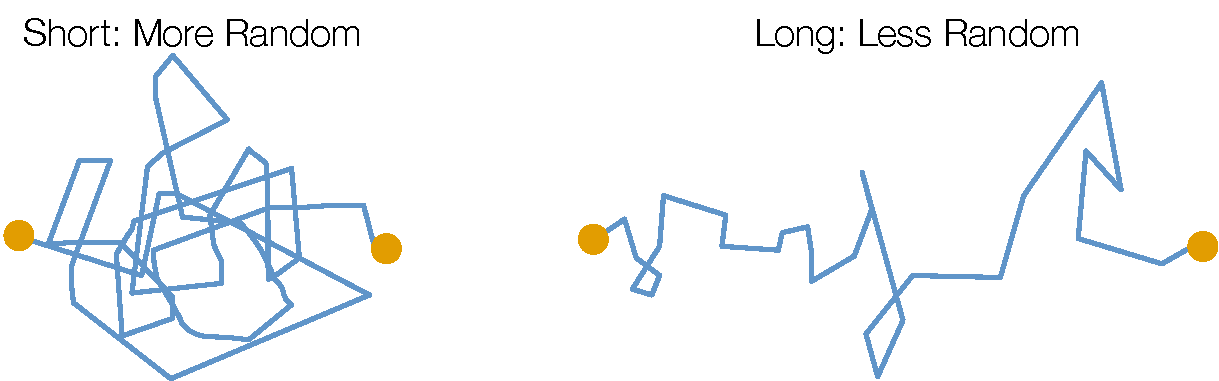
\includegraphics[width=\textwidth]{Short_and_Long_Comparison}
\caption{The reason polymers have a negative thermal expansion coefficient is because of entropy: their are more ways for the polymer to wiggle around when it isn't stretched out. We'll get quantitative about this in stat mech}
\label{shortLongEntropy}
\end{figure}
Yes! Indeed, this is observed in many systems. This happens when molecules gain degrees of freedom as the system size decreases. One examples is in polymers: there are more configurations when the chains in a polymer are bent. Thus as temperature increases, polymers tend to shrink!


\subsection{Check in: What you should be able to do by now}

\begin{enumerate}[(1)]
\item Identify work terms
\item Construct the relevant thermodynamic potential: see (\ref{LegendreTransforms})
\item Define equilibrium (internal degrees of freedom consistent with boundary conditions) 
\item Define the relevant properties: see (\ref{systematicWayDerivatives})
\item Relate thermodynamic quantities and thus variations: see (\ref{howToDerive})
\end{enumerate}


\subsection{Equilibrium Conditions for Multicomponent Systems}\label{eqMultiComponent}
Let's return to systems where we consider the mole numbers. We can write $dU$ for a multicomponent system as
\eqs
dU = TdS - PdV + \sum_i \mu_i dn_i
\eqe
where $\mu_i = \left(\frac{\partial U}{\partial n_i}\right)_{S,V,n_{i\neq j}}$ is the chemical potential of a species.  If we have a 2-phase system, we will have $S^{(1)}, V^{(1)}, \{n_j^{(1)}\}$ describing the first and $S^{(2)}, V^{(2)}, \{n_j^{(2)}\}$ describing the second.  We know
\eqs
\partial S^{(1)} &= -\partial S^{(2)}\\
\partial V^{(1)} &= -\partial V^{(2)}\\
\partial n_j^{(1)} &= -\partial n_j^{(2)}
\eqe
where $j=[1,...,r]$.  Meanwhile
\eqs
U &=\sum_{\alpha=1}^v U^{\alpha}\\
S&= \sum_{\alpha=1}^v S^{\alpha}\\
V&= \sum_{\alpha} V^{\alpha}\\
N&= \sum_{\alpha} n^{\alpha}\\
\eqe
\eqs
d U = \sum_\alpha T^{(\alpha)} (d S)^\alpha - P^{(\alpha)} (d V)^\alpha + \sum_{j=1}^v \mu_j (d n_j)^\alpha
\eqe
This is the first order displacement of $U$.  If the system is at equilibrium, $d U \geq 0$.  If true equilibrium, $d U |_{S,V,n}= 0$.  For a single homogeneous phase, $T, P, \mu$ are constant throughout the phase. Put more generally, the takeaway here is that if the extensive variables are allowed to vary independently of one another (i.e. the exchange of extensive variables between subsystems is uncoupled, just as charge is not coupled to mass flow in say, a battery), then the intensive variables in any subsystem must be the same as in any other subsystem.  If the pressures aren't equal, then the higher pressure subsystem will expand into the lower pressure subsystem, higher temperature subsystems will exchange heat with lower temperature subsystems, etc. Conceptually this means:
\begin{itemize}
\item we always formulate the conditions for equilibrium in terms of the intensive variables.
\item we can supply a bunch of constraints on the intensive variables of the different phases: they all need to be equal to one another. We derive these constraints in the next section.
\end{itemize}
If the exchange of extensive variables is coupled, it is the coupled sum of the the intensive variables that needs to be constant throughout a system at equilibrium. For example, if mass flow is coupled to charge exchange, then the electrical potential is coupled to the chemical potential of some species, and its electrochemical potential is homogeneous. If we denote $\mu^*$ as the electrochemical potential, it is easy to show that
$\mu^*=\mu+z F\phi$ must be constant across a system, where z is the charge on the species, F is Faraday's constant, and $\phi$ is the electrical potential.\\

\subsection{Constraints from equilibrium of heterogeneous systems: the Gibbs phase rule} \label{phaseRule}
For a system of $n$ well-behaved algebraic equations with $m$ variables, we may define the number of variables which can be freely assigned without invalidating (i.e. overspecifying) the system as:
\eqs f=m-n \eqe
We call $f$ the degrees of freedom of the system of equations. We define a phase as a part of a system which is measurably distinct in terms of its thermodynamic variables from another part of the subsystem.

When multiple phases are in equilibrium with each other, their intensive variables are constrained to vary with one another. One example would be a unary system where the liquid is in equilibrium with its vapor. We know that the temperature and pressure of the gas and liquid need to be the same at equilibrium, and that if we raise the temperature of the liquid, we increase the vapor pressure of the gas for it to remain in equlibrium with the liquid. Note that these are examples of \emph{constraints}: the liquid is \emph{constrained} to be at the same temperature and pressure as the gas, and the vapor pressure is \emph{constrained} to adjust itself when the temperature is adjusted. Clearly, there is a non-trival coupling between the intensive variables in the different phases. \textbf{The Gibbs phase rule expresses the number of degrees of freedom for the intensive variables when you have multiple phases at equilibrium}. The derivation of the phase rule thus amounts to counting the possible variations of the intensive variables and then subtracting the constraints upon these variables due to equilibrium among the different phases.
As stated above, we formulate the equilibrium between the different phases in terms of their intensive variables. Let there be $p$ phases, and let there by $c$ components in the system. We know that in each phase $\alpha$, a Gibbs-Duhem equation must hold:

\eqs
S^{\alpha }\text{dT}^{\alpha }-V^{\alpha }\text{dP}^{\alpha }+\underset{i=1}{\overset{c}{\Sigma }}N^{\alpha }\text{d$\mu $}_i^{\alpha }=0\eqe

Hence, for each phase, there are \textit{ c} + 1 independent intensive variables, which we can write in terms of $T^{\alpha },P^{\alpha }$, and the $c-1$ independent chemical potentials: $\mu _i^{\alpha}$. The number of variables is thus the number of phases times $c + 1$: 
\eqs m = p(c + 1) \eqe
The number of constraints from the intensive variables being equal to each other in each phase (such as $\mu_i^\alpha = \mu_i^\beta$, $T^\alpha=T^\beta$) is the number of intensive variables in each phase
times the number of phases minus 1:
\eqs n = (p - 1)(c + 2) \eqe

Then the number of independent variations of the intensive variables is thus (if one allows temperature and pressure to vary): 
\eqs f = m - n = c - p + 2 \text{ (}T\text{ and }P \text{ can vary)} \eqe
If, instead, one considers a system at constant pressure, you get:
\eqs f = c - p + 1 \text{ (}P \text{ specified)} \eqe
If temperature and pressure are both specified, you get:
\eqs f = c - p \text{ (}T\text{ and }P  \text{ specified)}\eqe
These are all versions of the Gibbs phase rule. It has important implications for the possible shapes of phase diagrams, which we will describe in section \ref{elementalPhaseDiagrams}.



% If there are $v$ phases coexisting (at equilibrium and constant $T, P$ (+2 equations)), then
% \eqs
% \mu_i^{(\alpha)} (T,P,x_1^\alpha,... x_{r-1}^\alpha) = \mu_i^{(\gamma)} (T,P,x_1^\gamma,... x_{r-1}^\gamma)
% \eqe
% and so $1 \leq \alpha < \gamma \leq v$ (for the number of phases, and for the number of species we have $1 < i < r$.  Ultimately, there are $r(v-1)$ equations for the chemical potential.

% \un{Gibbs Phase rule:}  The thermodynamic degrees of freedom $f$ is
% \eqs
% \boxed{f = 2 + r - v}
% \eqe
% be careful to note that we are using $x_i = \frac{n_i}{n_T}$ (the mole fraction) so the sum of the fractions should be equal to 1.  For example, in a one component system $r=1$ and we will fix $T,P$.  This results in 2 independent variables to describe our equilibrium (if no coexisting phases).\\

\subsection{Stability Conditions on the free energy} 
Here, we use a Taylor expansion to make some insights into the shape of $U$, and thus its Legendre transforms. $U$ can be expressed as a Taylor expansion in the extensive variables as:
\eqs
(\Delta U)_{S,V,n_j} = d U + d^2 U + ... > 0\\
\eqe
At equilibrium, we know that $d U = 0$. Therefore $dU \approx d^2U > 0$.  Thus, if we know that the second-order terms in a Taylor expansion of $U$ should all be positive to guarantee $U$ is minimal. More concretely, this corresponds to the case where one subsystem exchanges some amount of an extensive variable with another subsystem, such that the total amount of the extensive variable is conserved. To be at equilibrium, a system must be stable to such perturbations, as illustrated in figure \ref{stability}. 
\begin{figure}[h]
\centering
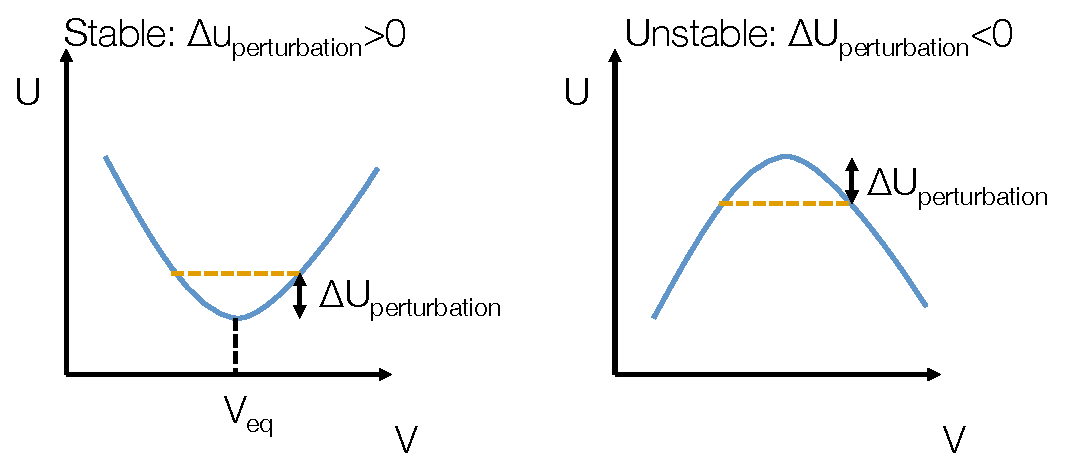
\includegraphics[width=\textwidth]{StabilityWRTPerturbations}
\caption{An illustration of a stable and unstable system with respect to volume perturbations. In the unstable case, subsystems can exchange volume and lower the energy of the systems. We call such instabilities to minute perturbations spinodal instabilities, and they evolve by special kinetics, termed spinodal decomposition.}
\label{stability}
\end{figure}

To illustrate this mathematically, we'll consider composite system with a diathermal wall\footnote{Reminder: heat can be exchanged, but $n$, $V$, cannot be exchanged.}, and then fix $S,V,n$:
\eqs
d S &= d S^{(1)} + d S^{(2)} = 0\\
d V^{(1)}&= d V^{(2)} = 0\\
d n^{(1)} &= d n^{(2)} 
\eqe
then the variation in $U$ becomes:
\eqs
d^2 U&= d^2U^{(1)} + d^2 U^{(2)}\\
&= \frac{1}{2}\frac{\partial^2U}{\partial S^{(1)2}}(d S^{(1)2}) + \frac{1}{2}\frac{\partial^2U}{\partial S^{(2)2}} (d S^{(2)2})
\eqe
Substituting in our known derivatives of $U$:
\eqs
\left(\frac{\partial^2U}{\partial S^{2}}\right)_{V,n} &= \left(\frac{\partial T}{\partial S}\right)_{V,n} = \frac{T}{c_V}\\
\partial^2U &= \frac{1}{2}(d S^{(1)2})\left[\frac{T^{(1)}}{c_V^{(1)}} + \frac{T^{(2)}}{c_V^{(2)}}\right]\\
T\left[\frac{1}{c_V^{(1)}} + \frac{1}{c_V^{(2)}}\right] &\geq 0\\
\eqe
Thus we get the result that $c_V \geq 0$. There is nothing special about the heat capacity, all other double derivatives of $U$ with respect to a single variable obey they same conditions; $U$ is concave up with respect to all the extensive variables.%Mathematically, $\frac{\partial^2f}{\partial x^{2}} > 0$ means we have convex upward (or convex positive) and likewise if $\frac{\partial^2f}{\partial x^{2}} < 0$ it is convex downward (convex negative).

\subsection{Phase stability}
$G$ is minimal at equilibrium for a constant T, constant P system, so it would be useful to translate this knowledge of the shape of $U$ to a more experimentally relevant potential. There are similar guarantees on the second derivatives of G. 
If we imagine that each phase/state of matter has its own free energy curve $G(T)^{\alpha},G(T)^{\beta},...$, then \emph{the equilibrium free energy is simply the lower envelope of the free energy curves of the possible phases}. This is shown in Figure \ref{phaseGCurves}.
\begin{figure}[h]
\centering
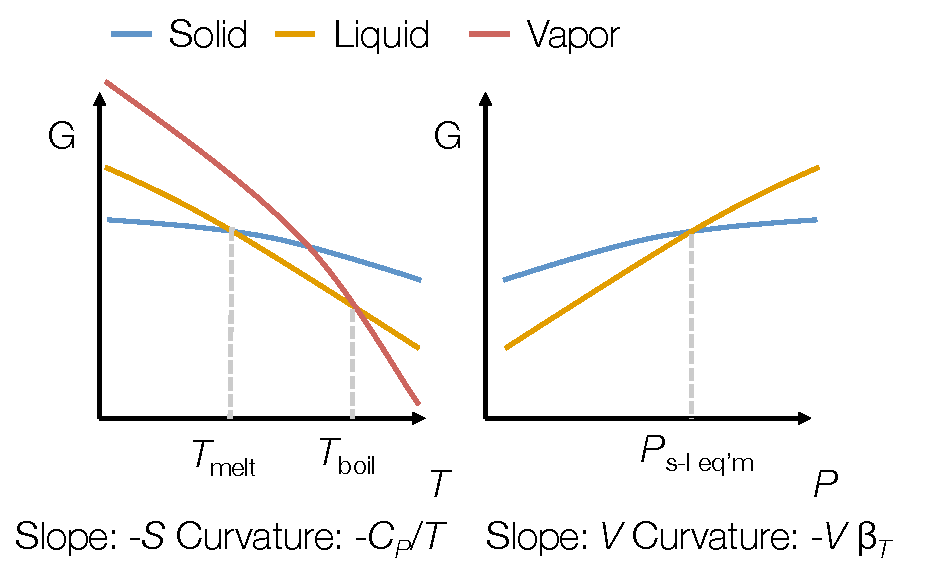
\includegraphics[width=12cm]{G_Curves_For_Phases}
\caption{An illustration of thermodynamically consistent curves for the free energy of phases as a function of T and P which obey the stability criteria.}
\label{phaseGCurves}
\end{figure}

Getting more quantitative, we can follow a similar line of thought as before for $U$. If there are two possible phases $\alpha$ and $\beta$, then at equilibrium between 2 phases, their free energies must be equal as shown in Figure \ref{phaseGCurves}
\eqs G^\alpha &= G^\beta %\\ \Delta G &= 0
\eqe
We can also read off the first derivatives of G: $\frac{\partial G}{\partial T}|_P = -S$ and $\frac{\partial G}{\partial P}|_T = V$. These hold for both phases. %$\alpha$ or $\beta$.  
Therefore, as a system passes through a two phase equilibrium, it should exhibit a discontinuity in its volume and entropy ($\Delta V_{\phi T}$, $\Delta S_{\phi T}$).
\eqs
\left(\frac{\partial G}{\partial T}\right)_P &= - S\\
\left(\frac{\partial^2 G}{\partial T^2}\right)_P &= -\left(\frac{\partial S}{\partial T}\right)_P = -\frac{c_P}{T} <0\\
\left(\frac{\partial G}{\partial P}\right)_T &= V\\
\left(\frac{\partial^2 G}{\partial P^2}\right)_T &= -\beta_T V <0\\
\eqe
For example, if we plot $G(T)$ for water, at 1atm of pressure and $G(T)$ for solid water and $G(T)$ for water vapor, we will see that at lower temperatures $G(T)$ for the solid is lowest, then at higher $T$, $G(T)_\text{water}$ becomes lower, and finally at even higher $T$ $G(T)_\text{vapor}$ is the lowest.  The derivatives of $G(T)$ get steeper from solid to liquid to vapor and are all negative, because $S_\text{solid} \ll S_\text{liquid} \ll S_\text{gas}$.


%With $T,P$ fixed and a closed system, we want to know ``what phase is stable?''  Since $T,P$ are fixed, we want to do a Legendre transform to $G$ so that $dG = 0$ for our equilibrium condition.  

%%%%%%%%%%%%%%%%%%%%%%%%%%%%%%%%%%%%%%%%%%%%%%%%%%%%%%%%%%%%%%%%%%%%%%%%%%%%%%%%%%%%%%%%%%%%%%%%%%%%%%%%%%%%%%%%%%%%%%%%%%%%%%%%%%%%%%%%%%%%%%%%%%%%%%%%%%%%%%%%%%%%%
%%%%%%%%%%%%%%%%%%%%%%%%%%%%%%%%%%%%%%%%%%%%%%%%%%%%%%%%%%%%%%%%%%%%%%%%%%%%%%%%%%%%%%%%%%%%%%%%%%%%%%%%%%%%%%%%%%%%%%%%%%%%%%%%%%%%%%%%%%%%%%%%%%%%%%%%%%%%%%%%%%%%%
\section{Lecture - September 25, 2014}
From last time, we looked at the plot of $G$ vs temperature $T$ for gaseous, liquid, and solid phases, finding that at low-T $G_\text{solid} < G_\text{liquid} <  G_\text{vapor}$, at $T$ greater than the melting temperature $G_\text{liquid} < G_\text{solid} <  G_\text{vapor}$, and then at $T$ greater than boiling $G_\text{vapor} < G_\text{liquid} <  G_\text{solid}$.  What is our $T_B$ (boiling temp.)?
\eqs
\Delta G_{l\rightarrow v}(T_B) = 0
\eqe
We know $\Delta H_{l\rightarrow v} = 44$ kJ/mol, $\Delta H_{l\rightarrow v} = 120$ J/mol, and $T_B = \frac{\Delta H_{l\rightarrow v}}{\Delta S_{l\rightarrow v}} = 370 K$.  How do we evaluate $\Delta G_{l\rightarrow v}(T)$?  We know that $\Delta S_{l\rightarrow v} = \frac{\Delta H_{l\rightarrow v}}{T_{\phi T}}$ at the phase transformation.
\eqs
\Delta G_{l\rightarrow v}(T) &\approx \Delta H - T \Delta S\\
&= \Delta H_{\phi T}-T\frac{\Delta H_{\phi T}}{T_{\phi T}} = \Delta H_{\phi T}(1-\frac{T}{T_{\phi T}})
\eqe
Remember to check your $\Delta c_P$.  If this is not correct, try $c_P^{l}$ or $c_P^{v}$.\\

\subsection{Ehrenfest classification of $\phi T$ (phase transitions)}
Since free energies curves of individual phases are continuous, the equilibrium free energy which consists of the lower envelope of all of these curves is also continuous. However, the derivatives of the equilibrium free energy curve will have discontinuities where different curves intersect, giving rise to a convenient way to describe phase transformations. 

The \textbf{Ehrenfest Classification of phase transitions} states that phase transitions can be uniquely identified by discontinuities in the derivatives of the appropriate free energy. First order transitions display discontinuities in the first order derivatives (volume, mole number, and entropy), while second order transitions display continuous first derivatives but discontinuties in the curvature of G (i.e. things like compressibilities and heat capacities are discontinuous).
\un{1st order}:  The first derivative of the potential is discontinuous (S, V, ...)\\
\un{2nd order}:  The second derivative of the potential is also discontinuous (but this implies that the first derivative is not)\\
Classifications beyond second order usually are not made, but presumably third-order phase transitions exist under the Ehrenfest classification, they just aren't as useful in real life, so we don't bother talking about them.

%\un{3rd order}: Third derivative of the potential...\\
\subsection{Elemental Phase Diagrams} \label{elementalPhaseDiagrams}

A \un{phase diagram} is a map of the conditions under which different phases are stable at equilibrium.\\
As described in sections \ref{eqMultiComponent} and \ref{phaseRule}, the intensive variables are a natural way to describe equilibrium between phases. As such, we will first talk about phase diagrams which have intensive variables as their axes, in particular, we begin with the simple case of $T$-$P$ phase diagrams for one-component systems, shown in Figure \ref{phaseDiagramCO2} for $\text{CO}_2$. 
% \begin{figure}
%   \centering
%   \def\svgwidth{\columnwidth}
%   \input{Carbon_dioxide_pressure_temperature_phase_diagram.pdf_tex}
%   \caption{The P-T phase diagram of $\text{CO}_2$. Image courtesy of \href{https://commons.wikimedia.org/wiki/File:Carbon_dioxide_pressure-temperature_phase_diagram.svg}{wikimedia commons}\footnote{Attribution is cool, even if the the image is copyleft}}
%   \label{phaseDiagramCO2}
% \end{figure}
\begin{figure}[h]
\centering
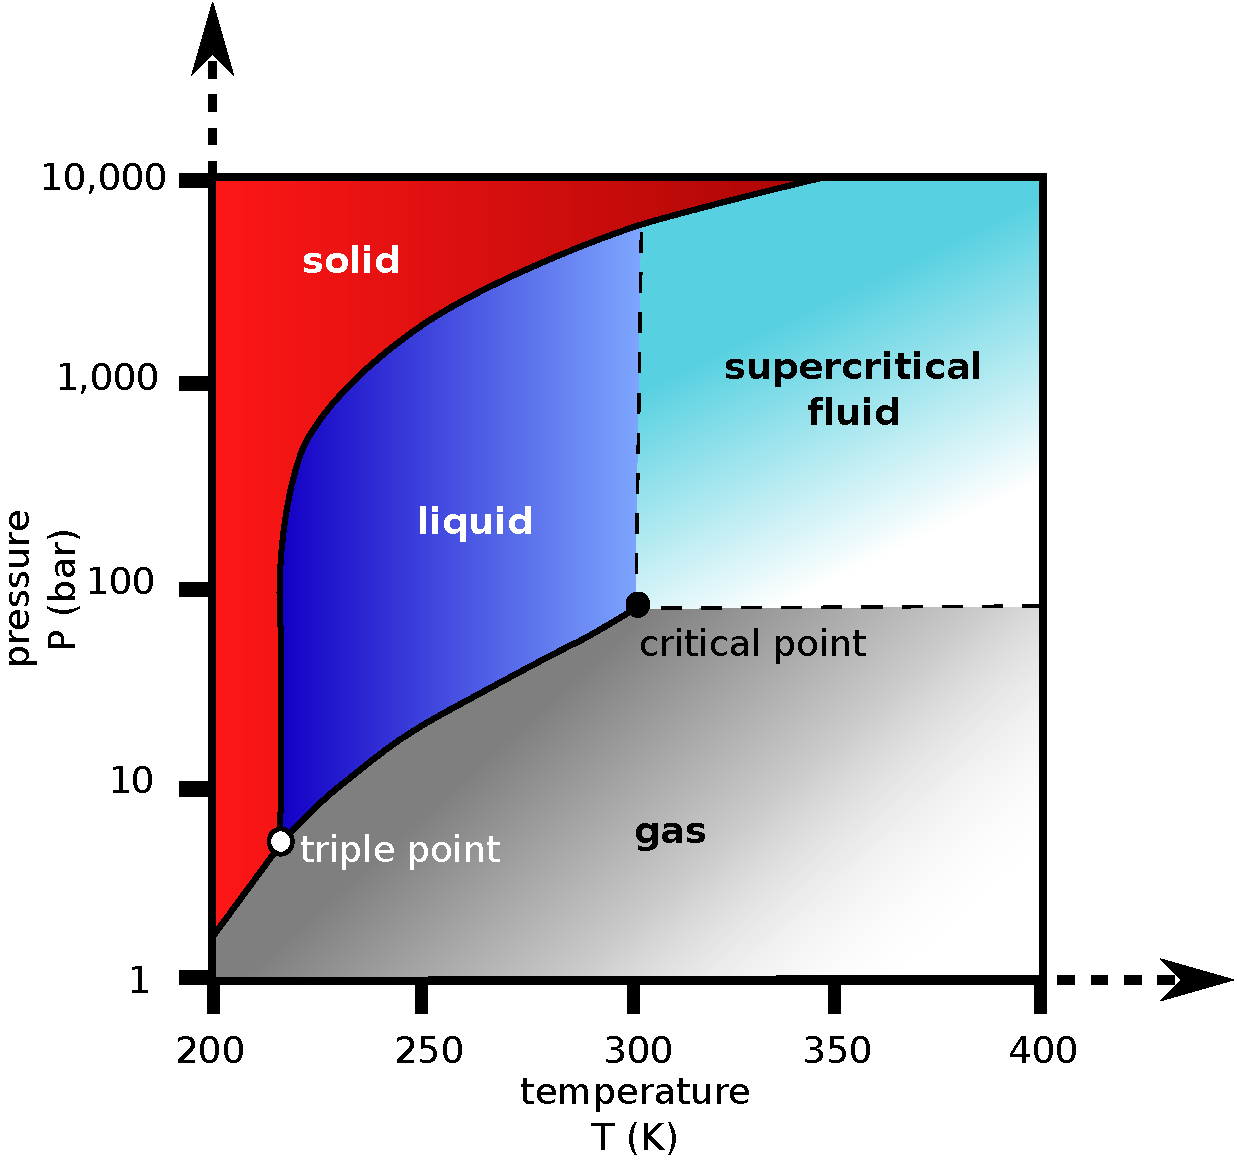
\includegraphics[width=10cm]{Carbon_dioxide_pressure_temperature_phase_diagram2.pdf}
\caption{The P-T phase diagram of $\text{CO}_2$. Image courtesy of \href{https://commons.wikimedia.org/wiki/File:Carbon_dioxide_pressure-temperature_phase_diagram.svg}{wikimedia commons}}%\footnote{Attribution is cool, even if the the image is copyleft}
\label{phaseDiagramCO2}
\end{figure}
% \begin{figure}[h]
% \centering
% \includegraphics[width=10cm]{CO2andHydrogenPD}
% \caption{\textbf{A} The P-T phase diagram of $\text{CO}_2$. Images courtesy of \href{https://commons.wikimedia.org/wiki/File:Carbon_dioxide_pressure-temperature_phase_diagram.svg}{wikimedia commons}}%\footnote{Attribution is cool, even if the the image is copyleft}
% \label{phaseDiagramCO2}
% \end{figure}

The open areas in Figure \ref{phaseDiagramCO2} correspond to single-phase regions, the lines to two-phase regions, and the intersection of lines to three phase regions, called triple points. A special point, called a critical point, marks a special case where it is no longer possible to distinguish between the two phases for which there was previously a border\footnote{We'll talk more about the meaning of critical points and the interesting phsyics which occur at criticality in statisttical mechanics.}.

\textbf{Exercise}: Prove using the phase rule that for a single-component system, the one-phase regions must be two-dimensional, the two-phse regions must be one-dimensional, and the three-phases regions must occur at a point in $T$-$P$ space.

One thing that is pretty universal about phase diagrams is that the pressures are really high compared to the pressures we normally think about; note the logarithmic scale in Figure \ref{phaseDiagramCO2}, and the fact that 1 bar = 0.1 MPa. We demonstrate why large pressures are needed to effect phase stability with an order of magnitude comparison: we'll calculate the work done per mole during a phase transition with some change in volume for `normal' pressures:
%How much does pressure affect the solid phases stability?
\eqs
\Delta W = P \cdot \Delta V\\
%\frac{\partial G}{\partial P}|_T = V
\eqe
A typical molar volume for an element is $V = 5 \cdot 10^{-6}$m\three/mol, and a large change in volume for condensed phases is on the order of 10\%, $\Delta V = 5 \cdot 10^{-7}$ m\three/mol. A large pressure would be 100 MPa, as this is the order of magnitude when most metals yield. Then $\Delta W = 100\cdot 10^{6} \cdot 5 \cdot 10^{-7} = 50 \text{J/mol} \approx 0.5$ meV. Let's compare this to the amount of energy it takes to heat an element by one degree K, $c_V\approx c_P \approx$ 25 J/mol/K. Therefore, we see that changes of a few degrees K cause the free energy to change the same amount as large changes in volume at rather high pressures. Thus, we expect that in order to appreciably change phase behavior that often takes place via changes of hundreds of degrees K, we will need to apply extremely large pressures, often on the order of tens to hundreds of GPa. This will become more quantitative in the next section.

%Now lets think about \un{iron}, which prefers a phase with smaller sensitivity to volume change (more FCC).  This is less sensitive to changes in pressure ($\Delta P$).  $G_\text{hcp} \approx G_\text{bcc}$ at low $P$?

%\un{Sulfur}: Up to 8 valencies, anions are $S^{2-}$.

\subsection{Determining Phase Diagrams}
Here we demonstrate that the slopes of the lines on phase diagrams are dictated by thermodynamics, and that you can usually guess them pretty well with a bit of knowledge. %Given a pressure vs temperature ($P$ vs. $T$) curve with a phase $\alpha$ above and $\beta$ below, we want to find the equation for our coexistence line.  $G_{T,P}^\alpha = G_{T,P}^\beta$ results in $dG_{T,P}^\alpha = dG_{T,P}^\beta$ and we have
We know that two phases are at equilibrium at a given temperature and pressure when their free energies are equal, $G_{T,P}^\alpha = G_{T,P}^\beta$. If we change the experimental conditions a bit, the phases will only remain in equilibrium if the free energy change of $\alpha$ is equal to the free energy change of $\beta$, $dG_{T,P}^\alpha = dG_{T,P}^\beta$. Expanding this expression gives:
\eqs
-S^\alpha dT + V^\alpha dP = -S^\beta dT + V^\beta dP
\eqe
This can be manipulated to give insight into the slope of the phase boundary in T-P space. Defining the differences in volume and entropy between the two phases and simplifying gives: %at the phase transformation $\alpha \rightarrow \beta$
\eqs
\Delta V^{\alpha \rightarrow \beta} &= V^\beta - V^\alpha\\
\Delta S^{\alpha \rightarrow \beta} &= S^\beta - S^\alpha
\eqe
\eqs \boxed{
\frac{dP}{dT} = \frac{\Delta S^{\alpha \rightarrow \beta}}{\Delta V^{\alpha \rightarrow \beta}}
}\eqe
This is known as the \emph{Clausius-Clapeyron relation}. It is commonly expressed in terms of the more easily-measured enthalpy changed of the phase transformation, $\Delta H^{\alpha \rightarrow \beta}$. This is possible because at a phase transformation, 
\eqs
\Delta G &= 0 
&= \Delta H^{\alpha \rightarrow \beta} - T^{\alpha \rightarrow \beta}\Delta S^{\alpha \rightarrow \beta} %&= \frac{\Delta H^{\alpha \rightarrow \beta}}{T^{\alpha \rightarrow \beta}}\\
\eqe
so we can eliminate $\Delta S^{\alpha \rightarrow \beta}$:
\eqs
\frac{dP}{dT} &= \frac{\Delta H^{\alpha \rightarrow \beta}}{T^{\alpha \rightarrow \beta} \Delta V^{\alpha \rightarrow \beta}}\\
\eqe
This relation actual tells us a very simple thing: if the temperature changes a bit when two phases are at equilibrium, the resulting difference in free energies is $\Delta S^{\alpha \rightarrow \beta}dP$. If the phases are to remain at equilibrium, a compensating change in the free energy due to pressure must be made: $-\Delta V^{\alpha \rightarrow \beta}dT$, so the rate at which the pressure changes with respect to temperature along a phase boundary is proportional to the ratio of their conjugates.

\subsection{Example: solid to liquid transition}
Here we just put some numbers to the Clausius-Clapeyron relationship for liquid-solid relationships so that you can get a feel for some numbers. 
\eqs
\Delta S &= S_l - S_s\\
\Delta V &= V_l - V_s
\eqe

\underline{How much $\Delta P$ is required to raise the melting point of Pb by 10\degree C?}
\eqs
\Delta H_m &= 4810 \text{J/mol}\\
T_M &= 600 K\\
v_l &= 19.47 {\text{cm}^3\text{/mol}}\\
v_s &= 18.92 {\text{cm}^3\text{/mol}}\\
\eqe
and so
\eqs
\frac{dP}{dT} &= \frac{\Delta H_M}{T_M\Delta V}\\
\Delta P &= \frac{\Delta H}{T_M\Delta V}\Delta T_M = 14.5 \text{ MPa}
\eqe

Most of the time $\Delta S > 0$ since liquids have higher entropy than solids.  If $\Delta V > 0$, $\frac{dP}{dT} > 0$, then the solid/liquid line will have a positive slope.  This is the case for most solid-liquid equilibria, as the solid is usually more dense than the liquid. There are some technologically relevant exceptions where $\Delta V < 0$.  These mostly occur in directionally-bonded solids, such as \href{http://commons.wikimedia.org/wiki/File:Phase_diagram_of_water.svg}{water}, \href{http://commons.wikimedia.org/wiki/File:Phase_diagram_of_silicon_(1975).png}{Si}, and \href{http://commons.wikimedia.org/wiki/File:Phase_diagram_of_germanium_(1975).png}{Ge}, but can occur for metallic elements such as \href{http://commons.wikimedia.org/wiki/File:Phase_diagram_of_gallium_%281975%29.png}{Ga} at low pressures.

Typical slopes:  For solid to liquid, we get $\Delta H = 10$ kJ, $\Delta V = 1$ cc/mol, and the slope is large, with the sign determined by the volume change (+/-).  For solid to gas,  $\Delta H = 100$ kJ, $\Delta V = 10^4$ cc/mol (~10 Liters), and the slope is small, but positive.

%%%%%%%%%%%%%%%%%%%%%%%%%%%%%%%%%%%%%%%%%%%%%%%%%%%%%%%%%%%%%%%%%%%%%%%%%%%%%%%%%%%%%%%%%%%%%%%%%%%%%%%%%%%%%%%%%%%%%%%%%%%%%%%%%%%%%%%%%%%%%%%%%%%%%%%%%%%%%%%%%%%%%%%%%%%%%%%%%%%%%%%%%%%%%%%%%%%%%%%%%%%%%%%%%%%%%%%%%%%%
%%%%%%%%%%%%%%%%%%%%%%%%%%%%%%%%%%%%%%%%%%%%%%%%%%%%%%%%%%%%%%%%%%%%%%%%%%%%%%%%%%%%%%%%%%%%%%%%%%%%%%%%%%%%%%%%%%%%%%%%%%%%%%%%%%%%%%%%%%%%%%%%%%%%%%%%%%%%%%%%%%%%%
\section{Lecture - September 26, 2014}
Simplified Clapeyron for the condensed phase and vapor equilibrium.  First we had the vapor as an ideal gas $V = \frac{RT}{P}$, and then second se approximated $\Delta V \approx V_g$
\eqs
\frac{dP}{dT} &= \frac{\Delta H}{T\Delta V}\\
&= P\frac{\Delta H_{\phi T}}{RT^2}\\
\frac{dP}{P}&= \frac{dT}{T^2}\frac{\Delta H}{R}\\
\ln(P) &= -\frac{\Delta_{\phi T}}{R} \frac{1}{T} + \text{constant}
\eqe

\un{Simplifying clapeyron}  For condensed phase/vapor\\
\eqs
\Delta V = V_v - V_l \approx V_v\\
\eqe
If the gas is ideal, we can use $V = \frac{RT}{P}$ and
\eqs
\frac{dP}{dT} &= \frac{\Delta H}{T \Delta V} = \frac{P \Delta H}{RT^2}\\
d(\ln(P)) &= -\frac{\Delta H}{R} (d(\frac{1}{T}))\\
\ln(P) &= -\frac{\Delta H}{R}\frac{1}{T} + \text{constant}
\eqe

\eqs
\Delta H_{\phi T}(T) &= \Delta H_{\phi T}(298) + \Delta C_p (T-298)\\
c_P^{v} &= a + bT + ...\\
c_P^{l} &= a' + b'T + ...\\
\Delta c_P &= A' + B'T+...\\
\eqe
Which leads to Antoine's equation:
\eqs
\log(P) = A - \frac{B}{T+C}
\eqe

\un{Are condensed phases really condensed?}\footnote{(i.e. Why do condensed phases have vapor pressures above them?)}\\
Take a look at the phase diagram for $\text{H}_2\text{O}$ in Fig \ref{PDH2O}.
\begin{figure}[h]
\centering
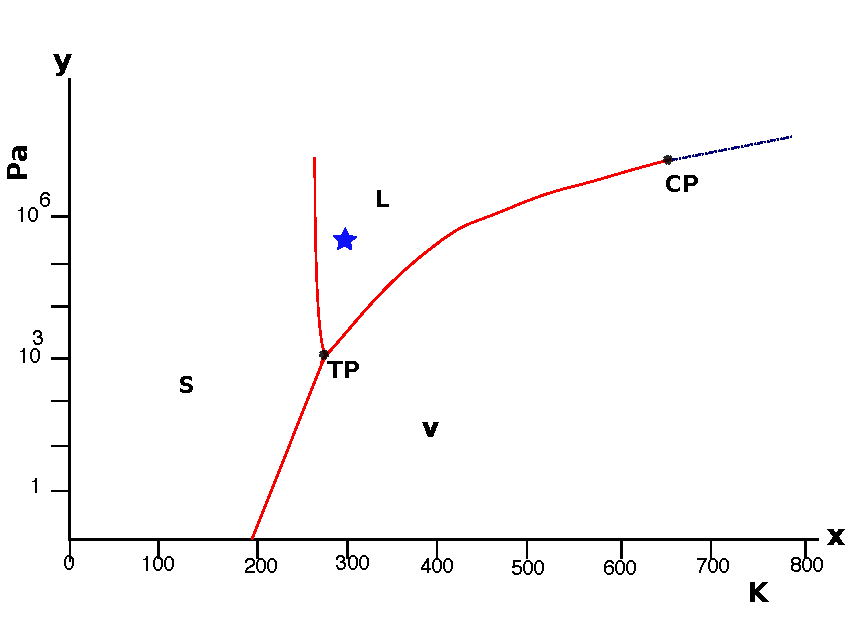
\includegraphics[width=8cm]{Water_phase_diagram}
\caption{A simplified phase diagram for water. The blue start is room temperature and pressure. Image from \href{https://commons.wikimedia.org/wiki/File:Water_phase_diagram.svg}{wikimedia commons}.}
\label{PDH2O}
\end{figure}
From looking at this phase diagram, one would think that at room temperature and pressure $\left(10^5\text{Pa}, 300 K\right)$, water should be
a single, liquid phase. Why, then, is there water vapor in the air around us? Well, this is because this phase diagram only considers \textit{unary
systems at constant pressure and temperature}, whereas water exists in systems where there are other elements in the vapor above it. Because liquid water at STP has some well-defined chemical potential of $\text{H}_2\text{O}$, the vapor above it must have enough $\text{H}_2\text{O}$ in it that it has the same chemical potential for $\text{H}_2\text{O}$.\\

The \textbf{vapor pressure} is defined as the partial pressure that a substance in the \un{condensed} phase will create in the vapor phase in equilibrium with it. Where a partial pressure is defined as:
\eqs
P_i = \frac{n_i}{n_\text{total}} P_\text{total}
\eqe
Because gases are ideal, if we have a liquid $A$ in a container with some other gas atmosphere, the partial pressure of the vapor $A$ is actually independent of the gas atmosphere. Vapor pressures are only defined by the chemical potentials in the condensed phases, in this case the liquid $A$.\\

\un{Example:} $P_{H_2O}(25^0) = 0.03$ atm.  At 45\degree it is 0.07 and at 100\degree it is 1 (boiling point).  The relative humidity is expressed by $\frac{P_{H_2O}}{P_{H_2O}^*}$.

Note: saturated water vapor does not behave like an ideal gas. If we have a system of 100\% pure humid air, then if we compress the system, the vapor pressure of the water will remain constant, and some of the water will condense. %If we have a system with an ice block inside of it, we will have water vapor forming and then to compensate for the energy (?) the ice cube will condense on the walls of the container.


\subsection{Le Chatelier-Braun principle}
 %If a system in equilibrium is subjected to constraints which displace the equilibrium, the transformation (reaction) proceeds in such  direction as to accommodate the constraints and \emph{partially} nullify their effects.
\un{Definition:} When a system, initially at equilibrium, is perturbed from its equilibrium state, the system adjusts itself to counteract the effect of the applied change in establishing a new equilibrium.\footnote{Callen provides a good discussion of this in Ch. 8-4 (p. 210)}\\
The most common example of this are in chemistry, such as when you add some reactant, A, to a system which was previously in some equilibrium governed by:
\eqs A+B \longleftrightarrow C+D\eqe
Adding some A acts as a\emph{ perturbation} to this system, and the system \emph{ adjusts itself} by reacting to partly eliminate this perturbation,
coming to a new equilibrium in the process.\footnote{Throwing away the thermo jargon: if you put a bit of $A$ in, some of that $A$ reacts, so the concentration of $A$ becomes less.} Thermodynamically, this is tantamount to increasing the chemical potential of A, with the forward reaction
acting to then homogenize this perturbation in the chemical potential. \footnote{Historical note: Le Chatelier and Braun discovered this principle independently,
so in 3.20 we give attribution to both of them!}

\subsection{Generalization of Clausius-Clapeyron}
The method to generate the Clausius-Clapeyron equation can be applied to any two sets of work terms, by taking the proper Legendre transform such
that the intensive variables of interest are the natural variables for the thermodynamic potential. For example, in the case of the Clausis-Clapeyron
equation, the intensive variables of interest were T and P, so we took $\phi $ = U-TS+PV, which turns out t be G. Along a phase boundary, this gave rise to the relation:
\eqs
\frac{\partial P}{\partial T}=\frac{\text{$\Delta $s}}{\text{$\Delta $v}}
\eqe
A similar relationship can be derived for a magnetic phase transition, taking
instead: $\phi $ = U - TS + PV - HM such that
\eqs \text{d$\phi $}=-S \text{dT}+V \text{dP}-M \text{dH}\eqe
for the system as a whole. We again consider the case where the system is composed of two phases in equilibrium with one another, and where want to move along a two-phase equilibrium boundary in T-H space such that the different thermodynamic potentials are ``changing'' at the same rate:
\eqs\text{d$\phi $}^1=\text{d$\phi $}^2\eqe
meaning:
\eqs
-S^1 \text{dT}+V^1 \text{dP}-M^1 \text{dH}-\left(-S^2 \text{dT}+V^2 \text{dP}-M^2 \text{dH}\right)=0
\eqe
For a system at constant pressure, we
can show that:
\eqs\left(\frac{\partial H}{\partial T}\right)_P=-\frac{\text{$\Delta $S}}{\text{$\Delta $M}}\eqe
In general, this can be written for any work term as:
\eqs\left(\frac{\partial Y_j}{\partial T}\right)_{Y_{i\neq j}}=-\frac{\text{$\Delta $S}}{\text{$\Delta $X}_j}\eqe
Where the intensive variables are on the left, and the extensive variables are on the right. Due to the weird sign convention with $P$, C-C relationships with $P$ have a negative sign.
% \eqs
% dU &= TdS + \sum_i y_i dx_i\\
% G &= U-TS - y_idx_i\\
% dG &= -SdT - \sum x_i dy_i
% \eqe
% Say the change in temperature is not equal to zero ($dT \neq 0$) and the change in other components isn't either ($dy_j \neq 0$, $dy_{i\neq j} = 0$).  How does the equilibrium change when varying those variables?
% \eqs
% \frac{dy_j}{dT}|_{y_{i\neq j}} = - \frac{\Delta S}{\Delta x_j}
% \eqe  

\subsection{Magnetic-induced phase transformation}
Let's put some numbers onto this new C-C relationship to get a sense of how temperature can affect the $T$-$H$ phase boundary.
\eqs
dU &= TdS + \mu_0 H dM\\
dG &= -SdT - \mu_0 M dH
\eqe
\eqs
\frac{dT}{dH} &= -\frac{\Delta M}{\Delta S}\\
\eqe
\eqs
\Delta M &= M_\text{ferro} - M_\text{para} \approx 4 \mu_B \approx 4 \cdot 10^{-5} \text{eV/Tesla}
\eqe
Where we assumed that the magnetization of the ferromagnetic material was 4 Bohr magneton per atom.  For spins, we can have two states, so 
\eqs
\Delta S = k_B \ln(2)
\eqe
Thus we can estimate our change in temperature with field
\eqs
\frac{dT}{dH} = -\frac{4 \cdot 10^{-5}}{8.617 \cdot 10^{-5} \cdot \ln(2)} = -0.66 \text{K/Tesla}
\eqe
Note: a Tesla is a \emph{huge} magnetic field, so we see that phase boundaries between magnetic phases are super strongly affected by temperature, making them hard to study well if you don't have good control over $T$.

\subsection{Thermoelasticity}
An application of a generalized Clausius-Clapeyron relationship is thermoelasticity. Thermoelasticity, or ``superelasticity'' is a recoverable strain far beyond what is normally expected for solids \footnote{Elastic deformation usually only occurs until around $\epsilon \approx 0.2\%$. Superelasticity permits reversible strains of up to 10\%}.  The phase transformation is typically induced by stress.  In the high-T phase, we have the A (austenite) phase.  In the low-T phase, we have M (martensite).
The stress-strain curves look like those in Fig \ref{superElasticity} \textbf{A}.

\begin{figure}[h]
\centering
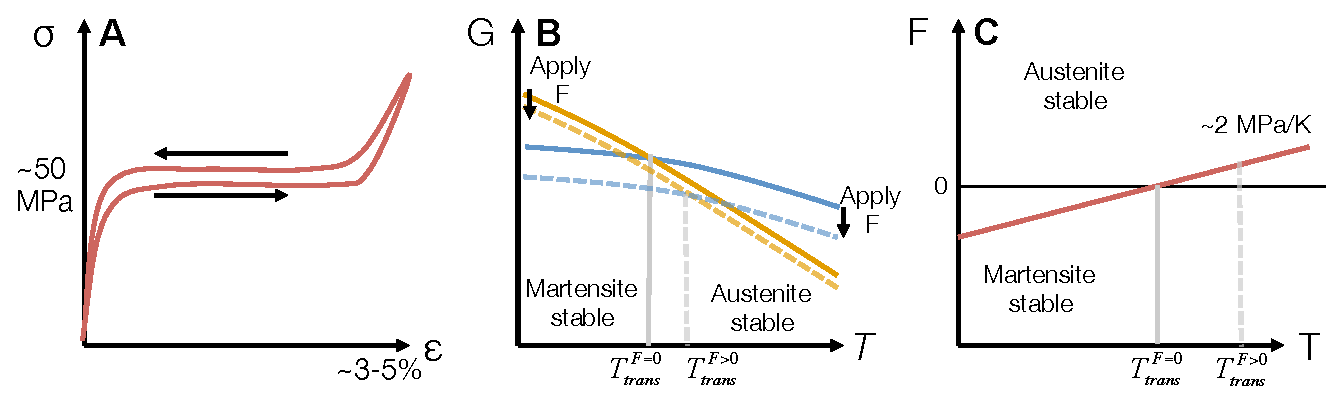
\includegraphics[width=\textwidth]{superelasticity}
\caption{\textbf{A} A typical stress-strain curve for a superelastic material. \textbf{B} Free energy curves for martensite and austenite as a function of temperature showing how the curves shift upon application of a stress \textbf{C} A simplified phase diagram for superelastic materials.}
\label{superElasticity}
\end{figure}

Keep in mind what you see in Fig \ref{superElasticity} \textbf{A}; a discontinuity in an extensive variable (length/strain) while an intensive variable is constant (force/stress). This is almost always a sign that changing the intensive variable induced a first-order phase transition.\footnote{Another example is when battery charge-discharge curves \href{http://i.stack.imgur.com/UkodS.gif}{exhibit a constant discharge voltage} for a large amount of current}

If we plot G vs. T, both phases exhibit downward slopes and negative curvature, as in Fig \ref{superElasticity} \textbf{B}. The higher entropy austenitic phase will have a larger, negative slope, and thus become stable at higher temperature. We want to investigate the effect of force on the temperature of the superelastic transition, so we set up our relevant potential:

\eqs
dU &= TdS + F dL\\
G &= U- T\cdot S - F \cdot L\\
L &= -\left(\frac{\partial G}{\partial F}\right)_{T_i}
\eqe
By applying a force and stretching the material, we move the $G\text{ vs. }T$ line downwards for both phases, but the the martensitic phase moves down more quickly than the parent phase due to the martensite's larger $L$. This relative movement is indicated by the dashed lines in Fig. \ref{superElasticity}\textbf{B}. The interesting thing is that because they don't move at the same rate, you get shifts in the transition temperature due to application of stress; there's a Clausius-Clapeyron effect here. Let's quantify it in the context of a specific system.\\

Say we're talking about Cu-Al-Zn at $T_0 = 300K$, $V \approx 8 \cdot 10^{-6}$ m\three/mol, $\Delta S \approx 1$ J/mol/K.  Now we write down a version of Clausius-Clapeyron:
\eqs
\frac{1}{A} \frac{dF}{dT} &= -\frac{\Delta S}{\Delta P}\frac{1}{A}\\
A \Delta P &= V_m \Delta \epsilon\\
\frac{d\sigma}{dT} &= -\frac{\Delta S}{V_m \Delta \epsilon} = (8 \cdot 10^-6 \cdot 7.5 \cdot 10^{-3})^{-1} = 1.66 \text{MPa/K}
\label{superElastCC}
\eqe
The resulting phase diagram is shown in Fig. \ref{superElasticity}\textbf{C}, it's just a line with a slope given by Eq. \ref{superElastCC}.

In general, what would be the heat involved if we apply a stress?
\eqs
H &= U+PV\\
dH &= \partial Q +VdP + F dl\\
(dH)_p &= (\partial Q)_P F dl
\eqe
Universal enthalpy
\eqs
H &= U - \sum y_i x_i\\
H' &= U + PV - Fl\\
(dH') &= (\partial Q)_P - l dF
\eqe
%%%%%%%%%%%%%%
%\subsection{EXAM 1 MATERIAL ENDS HERE}
%\begin{itemize}
%\item Test on Friday, 9:30am (\emph{not} 9:35am) to 10:55am (sharp) in Walker, Building 50.
%\item No recitation this week
%\item Thursday - pizza party office hours and review (TBD)
%\item Mike Gibson's office hours Monday and Wednesday 11:00am - 12:00am
%\item Lecture on Wednesday is a review (with office hours) and will be from 9:00am - 11:00am.
%\item Extra office hours?
%\end{itemize}
%
%%%%%%%%%%%%%%%%%%%%%%%%%%%%%%%%%%%%%%%%%%%%%%%%%%%%%%%
%\section{Lecture - September 29, 2014}
%\subsection{Open Systems}
%\eqs
%U &= TS - PV + \sum \mu_i N_i\\
%G &= U - TS + PV\\
%&= \sum \mu_i N_i
%\eqe
%If we extend what we have seen before for the various intensive properties, we can write down our second derivative charts again
%\begin{center}
%\begin{tabular}{c | c | c | c}
%& T & P & $n_i$ \\ \hline
%T & $-\frac{c_P}{T}$ & $\alpha_V V$& $-\bar{S_i}$ \\ \hline
%P & $\alpha_V V$ & $-\beta_T V$& $\bar{V_i}$ \\ \hline
%$n_i$ & $-\bar{S_i}$ & $\bar{V_i}$ & $\frac{\partial \mu_i}{\partial n_i}$
%\end{tabular}
%\end{center}
%where the extra second derivatives are from
%\eqs
%\frac{\partial^2 G}{\partial T \partial n_i} &= -\frac{\partial S}{\partial n_i}|_{P,T,n_{j\neq i}} = -\bar{S_i}\\
%\frac{\partial^2 G}{\partial P \partial n_i} &=\frac{\partial V}{\partial n_i} = \bar{V_i}
%\eqe
%A \un{partial molar quantity} $\bar{x_i}$ is given by
%\eqs
%\bar{x_i} = \frac{\partial x}{\partial n_i}|_{y,n_{i\neq j}}
%\eqe
%For a single component, we graphed our pressure vs. temperature plot (P vs T), indicating the regions of vapor, solid, and liquid.  In addition, we could plot pressure vs. partial molar volume (P vs $\bar{V}$) with isothermal lines.  At a phase change the volume would change discontinuously with pressure.\\
%
%Given a system open to two components A \& B, we know $dN_A = -dN_B$.  See notebook for binary phase diagram.  We will end up converting this over to a T vs. $\mu_B^*$ diagram.
%
%\eqs
%dU &= ... \mu_A dN_A + \mu_B dN_B\\
%&= (\mu_B - \mu_A) dN_B\\
%&= \mu_B^* dN_B
%\eqe
%\eqs
%d\phi = -S dT + VdP - N_B d\mu_B^* = 0\\
%\eqe
%\eqs
%\frac{dT}{d\mu_B^*} = -\frac{\Delta N_B}{\Delta S}
%\eqe
%(see notebook on two phase diagrams)
%
%\subsection{Molar Volume}
%\eqs
%\bar{V}_A = \frac{\partial V}{\partial n_A}|_{T,P}
%\eqe
%The density matters?  Lets add an interstitial atom B into a crystal lattice of A atoms.  If we have pure B ($x_A = 0$):
%\eqs
%\bar{V}_A(x_A = 0) &= 0\\
%\bar{V}_B(x_A=0) &= V_B
%\eqe
%If we have just pure A $(x_A = 1)$
%\eqs
%\bar{V}_B(x_A = 1) &= 0\\
%\bar{V}_A(x_A = 1) &= V_A
%\eqe
%Our partial molar volume can be either positive or negative.  Assume we have a container with H\2O$_{(l)}$ in it and we add MgSO\4, which will ionize to form MG$^{2+}$ and SO\4$^{2-}$.  The water interacts with the magnesium and shortens the distance between the water molecules.  Thus, $\bar{V}_{\text{MgSO}_4}$ is initially negative, and then at some saturation point
%
%%%%%%%%%%%%%%%%%%%%%%%%%%%%%%%%%%%%%%%%%%%%%%%%%%%%%%%
%\section{Readings}
%Taken from the Stellar site, \emph{An Introduction to Statistical Mechanics} by Hill, or \emph{Thermodynamics and an Introduction to Thermostatics} by Callen.
%
%\subsection{First-Order Phase Transitions ({Callen Ch. 9})}
%The shift of the equilibrium state from one local minimum to the other constitutes a \emph{first-order phase transition}, induced by changing temperature, or other thermodynamic parameters.  The two states between which a first-order phase transition occurs are distinct, occurring at separate regions of the thermodynamic configuration space.  The states between which a \emph{second-order phase transition occurs} are contiguous states in the thermodynamic configuration space.
%
%%%%%%%%%%%%%%%%%%%%%%%%%%%%%%%%%%%%%%%%%%%%%%%%%%%%%%%
\section{Review of Exam 1 materials}
First part of test is True/False questions.  An example of a question would be:\\

``A one component material undergoes a pressure induced phase transformation at $P_{\phi T}$.  The material has the same equation of state in both phases.  True or False?'' (20 questions like this)\\

``In the $\alpha$ phase, $\beta P = a + b \beta \mu$ ($\mu$ is the chemical potential, $\beta = 1/T$), in $\gamma$ phase, $\beta P = c + d (\beta \mu)^2$.  $a,b,c,d$ are positive functions of $\beta$, and we know $d > b$, $c < a$.  What is the density differences between $\alpha$ and $\gamma$ at the phase transformation?  What $P_{\phi T}$ does the transition happen at?''

\un{Solution:} We know that at the phase transformation $\mu_\alpha = \mu_\beta$ and $\beta^{(\alpha)} = \beta^{(\gamma)}$, and $\rho = 1/V$.

%\begin{enumerate}[(1)]
\subsection{Definitions}
\begin{itemize}
\item \bold{System:} Any collection of matter that can be uniquely identified and on which you can define macroscopic averages
\item \bold{Environment:}  Complement of the system
\eqs
[\text{Universe}] = [\text{Environment}] + [\text{System}]
\eqe
\item \bold{Extensive Variables:} Variables that scale with a system's size (volume, mass, number of particles, ...)
\item \bold{Intensive Variables:} Variables that do \emph{not} scale (pressure, temperature, chemical potential, ...)
\item \bold{Boundaries:} Define a system and its interaction with the environment
\item \bold{Adiabatic:} No flow of heat $\partial Q = 0$ and $PV^{\gamma} = \text{constant}$, where the $\gamma$ is determined by
\eqs
\gamma = \frac{c_P}{c_V} = \frac{f+2}{f}
\eqe
\item \bold{Conserved quantity}: A quantity dependent on variables that are \emph{constant}.  (In this class, we can assume the extensive parameters, except entropy $S$, are conserved.)
\item \bold{Reversible process}: Constant entropy process ($dS=0$)
\item \bold{Isochoric:} Constant volume $dV = 0$
\item \bold{Isentropic:} Constant entropy $dS = 0$
\item \bold{Isenthelpic:} Constant enthalpy $dH = 0$
\item \bold{Isothermal:} Constant temperature $dT=0$.  For an ideal gas, $U = U(T) = n c_V T$ where $c_V = \frac{3}{2} R$ for a monoatomic gas or $c_V = \frac{5}{2} n R$ for a diatomic gas.
\item \bold{Isobaric:} Constant pressure $dP = 0$
\item \bold{Equations of state:} Expression of intensive parameters in terms of independent extensive parameters (e.g. $T= T(S,V,N,...)$)
\item \bold{Relative Humidity:} $\frac{P_{H_2O}}{P_{H_2O}^*}$ where the numerator is the partial pressure of water vapor \emph{in the mixture} and the denominator is the \emph{equilibrium vapor pressure} of water.
\item \bold{The Fundamental Equation:}
\eqs
dU = TdS - PdV + \sum_i^k \mu_i dn_i + ...
\eqe
\item \bold{Heat Capacity:} The amount of heat that changes with changing temperature.  For example:
\eqs
c_V &= \left(\frac{\partial Q}{\partial T}\right)_V = \frac{d U}{d T}\\
c_P &= \left(\frac{\partial Q}{\partial T}\right)_P = \frac{d H}{d T}
\eqe
\item \bold{Dulong-Petit:} This is simply the relationships for $c_v$ and $c_p$ for monoatomic and diatomic gases.  For monoatomic gases, $c_v = \frac{3}{2} R$, for diatomic gases $c_v = \frac{5}{2} R$, and for both, $c_p = c_v + R$.
\end{itemize}


%%%%%%%%%
\subsection{Thermodynamic Laws}
\begin{enumerate}[(1)]
\item $dU = \partial W + \partial Q$.  If adiabatic, $dU = \partial W$
\item Reversible: $dS_\text{system} = \frac{\partial Q}{T}$\\
Irreversible: $dS_\text{system} = \frac{\partial Q}{T}$
\item As temperature $T$ approaches zero, the magnitude of entropy change ($dS$) in any reversible process is zero (Thus heat capacity at $T=0$ is zero also).
\end{enumerate}



%%%%%%%%%
\subsection{All the heat capacities, expansion coefficients, etc.}
\begin{enumerate}[(i)]
\item Coefficient of thermal expansions
\eqs
\boxed{\alpha = \frac{1}{V}\left(\frac{\partial V}{\partial T}\right)_P}
\eqe
\item Isothermal compressibility (sometimes denoted by $\kappa_T$)
\eqs
\boxed{\beta_T = -\frac{1}{V}\left(\frac{\partial V}{\partial P}\right)_T}
\eqe
\item Molar heat capacity at constant pressure (works similarly with volume):
\eqs
\boxed{c_{P} = \frac{1}{N}\left(\frac{\partial Q}{\partial T}\right)_{P} = \frac{T}{N} \left(\frac{\partial S}{\partial T}\right)_{P} = T\left(\frac{\partial s}{\partial T}\right)_{P}}
\eqe
\end{enumerate}
%%%%%
\subsection{Maxwell Relations}
\begin{enumerate}[(i)]
\item Find the extensive variables to be represented (i.e. T,P)
\item Convert to the appropriate energy (i.e. G(T,P))
\item Determine if there is a \un{sign difference} between the two extensive variables
\item Match both second derivatives
\end{enumerate}
%%%%%
\subsection{Gibbs-Duhem}
Results from comparing the partial derivative of the Euler equation $U = TS - PV + \sum\mu_i N_i$ to the first law.
\eqs
0=SdT - VdP + \sum N_i d\mu_i
\eqe
%%%%%
\subsection{Internal energy $U$, enthalpy $H$, Helmholtz $F$, and Gibbs $G$}
\begin{enumerate}[(i)]
\item H = U + PV
\item F = U - TS
\item G = U - TS + PV
\end{enumerate}
%%%%%
\subsection{Legendre Transforms:}
Given a potential and asked to make the other potentials (i.e. $U(S,X) = X^{-a}e^{bS}$)
\begin{enumerate}[(i)]
\item Find the equations of state (relate first derivatives to the conjugate variables you know they should be)
\item To eliminate a variable $S$ of conjugate pair $S,T$, do $\phi= U-TS$
\item Substitute values from equations of state to make sure new potential is in terms of appropriate variables
\end{enumerate}
%
\subsection{Some useful math identities:}
\eqs\boxed{
\left(\frac{\partial f}{\partial x}\right)_g = \left(\frac{\partial f}{\partial x}\right)|_y + \left(\frac{\partial f}{\partial y}\right)_x \cdot \left(\frac{\partial y}{\partial x}\right)_g}
\eqe
\eqs \boxed{
\left(\frac{\partial f}{\partial x}\right)_y \left(\frac{\partial x}{\partial y}\right)_f \left(\frac{\partial y}{\partial f}\right)_x = -1}
\eqe
Also just know the chain rule and inverse rule (pretty intuitive). \\ 

\bold{Variable reduction:}
\begin{enumerate}[1.]
\item Bring your thermodynamic potential to the numerator
\item Bring $S$ to the numerator and turn it into a heat capacity or use a Maxwell Relation
\item If needed, bring your volume to the numerator and turn it into a derivative of $T$ and $P$.
\item Relate heat capacities to what you know
\end{enumerate}

%%%%%%%
\subsection{Carnot Engines:}
Carnot engines really aren't two complicated.  The principles are completely derived from the first two principles at reversible equilibrium $dS = 0 = dS_1 + dS_2$ and $dU = 0 = \partial Q + \partial W$.  The different efficiencies are all just the quantities that \emph{you want to get out of your pump/engine/refridgerator}.  Let's begin:
\eqs
dS = dS_1 + dS_1 &= 0\\
\frac{\partial Q_1}{T_1} &= -\frac{\partial Q_2}{T_2}\\
\partial Q_1 &= -\partial Q_2 \frac{T_1}{T_2}
\eqe
and now with the first law
\eqs
dU = \partial Q_1 + \partial Q_2 + \partial W &= 0\\
(1-\frac{T_1}{T_2})\partial Q_2 = -\partial W
\eqe

\bold{Carnot Engine}:  Here we care about getting work \emph{out} by using a \emph{heat source}, so the efficiency is
\eqs
\mu_\text{engine} = \frac{-\partial W}{\partial Q_\text{hot}} = 1-\frac{T_L}{T_H} = \frac{T_H - T_C}{T_H}
\eqe
\bold{Heat Pump}: Here we care about \emph{extracting heat} by \emph{doing work} on the system.  The efficiency is then
\eqs
\mu_\text{pump} = \frac{-\partial Q_H}{\partial W} = \mu_\text{engine}^{-1} = \frac{T_H}{T_H-T_C}
\eqe
\bold{Refridgerator}: Here we want to maximize the amount of heat \emph{leaving} the cold system by \emph{doing work}.
\eqs
\mu_\text{refridgerator} = \frac{-\partial Q_C}{\partial W} = \frac{-\partial Q_H \frac{T_C}{T_H}}{-(1-\frac{T_C}{T_H})\partial Q_H}= \frac{-T_C}{-(T_H-T_C)} = \frac{T_C}{T_H-T_C}
\eqe

\bold{Carnot Cycle} (All use reversible work sources)
\begin{enumerate}
\item \un{Isothermal expansion} with \emph{hot} reservoir contact and reversible work
\item \un{Adiabatic expansion} with reversible work to $T_C$
\item \un{Isothermal compression} with \emph{cold} reservoir contact and reversible work
\item \un{Adiabatic compression} with reversible work to $T_H$
\end{enumerate}

\subsection{Le Chatelier-Braun principle}
\un{Definition:} If a system in equilibrium is subjected to constraints which displace the equilibrium, the transformation (reaction) proceeds in such  direction as to accommodate the constraints and \emph{partially} nullify their effects.

%%%%%
\subsection{Clausius-Clapeyron:}
The Clausius-Clapeyron equation is a way to characterize phase transformations between two phases of matter (of the same constituent material).  Know the \emph{generalized form} (below) and be able to derive it for new systems:
\eqs
\frac{dy_j}{dT}|_{y_{i\neq j}} = - \frac{\Delta S}{\Delta x_j}
\eqe  
\eqs\boxed{
\frac{dP}{dT} = \frac{\Delta H}{T\Delta V}}
\eqe
which, for an ideal gas and where $\Delta V = V_{(g)}-V_{(l)} \approx V_{(g)}$ leads to:
\eqs
\ln(\frac{P_f}{P_i}) = \frac{\Delta H}{n R}[\frac{1}{T_i}-\frac{1}{T_f}]
\eqe

\bold{Derivation:}
\eqs
d\underline{G}^\alpha &= d\underline{G}^\beta\\
-\underline{S}^\alpha dT + \underline{V}^\alpha dP &= -\underline{S}^\beta dT + \underline{V}^\beta dP\\
\Delta \underline{V}^{\alpha \rightarrow \beta} &= \underline{V}^\beta - \underline{V}^\alpha\\
\Delta \underline{S}^{\alpha \rightarrow \beta} &= \underline{S}^\beta - \underline{S}^\alpha\\
\Delta \underline{S}^{\alpha \rightarrow \beta}dT + \Delta \underline{V}^{\alpha \rightarrow \beta} dP &= 0\\
\frac{dP}{dT} &= \frac{\Delta \underline{S}^{\alpha \rightarrow \beta}}{\Delta \underline{V}^{\alpha \rightarrow \beta}}\\
\Delta \underline{S}^{\alpha \rightarrow \beta} &= \frac{\Delta \underline{H}^{\alpha \rightarrow \beta}}{T^{\alpha \rightarrow \beta}}
\eqe
plugging in we get the Clapeyron Equation, which defines the slope of our $P/T$ curve:
\eqs
\frac{dP}{dT} &= \frac{\Delta \underline{H}^{\alpha \rightarrow \beta}}{T \Delta \underline{V}^{\alpha \rightarrow \beta}}
\eqe

%%%%%
\subsection{Raoult's Law:}
Given a mixture of ideal liquids, the vapor pressure of each constituent liquid is equal to the vapor pressure of that liquid as a \emph{single component} multiplied by the concentration.  Thus, the total vapor pressure of the mixture is 
\eqs
P_\text{vap} = \chi_A p_A + \chi_B p_B + ... = \sum_i \chi_i p_i
\eqe

\subsection{Phase changes:}
You should be able to look at a $G$ vs. $T$ plot and rank the magnitudes of the entropy and heat capacity $c_P$ for the solid, liquid, and gas phases.  We can do this because
\eqs
\frac{\partial G}{\partial T} &= -S\\
\frac{\partial^2 G}{\partial T^2} &= \frac{-c_P}{T}
\eqe

\bold{Gibb's Phase Rule:} If there are $n$ phases of $r$ species coexisting at equilibrium and constant temperature and pressure, then there are $f$ degrees of freedom where
\eqs
f = 2 + r - n
\eqe

\bold{Binding Energy and Phase Change Rules}:\\

Richard's Rule:
\eqs
\Delta H_\text{fusion} = 9 T_\text{fusion}
\eqe
Trouton's Rule:
\eqs
\Delta H_\text{vaporization} = 90 T_\text{vaporization}
\eqe

For a reaction
\eqs
aA + bB \rightarrow cC + dD
\eqe
the enthalpy of reaction $\Delta_r^0$ is
\eqs
\Delta H_r^0 = c\Delta H_C^0 + d\Delta H_D^0 - b\Delta H_B^0 - a \Delta H_A^0
\eqe

\bold{Stable equilibrium criteria:}\\
At a relative minima or maxima, $dU = 0$.  Also, $d^2U > 0$, which guarantees a minima.  At a constant temperature and pressure, two phases are in equilibrium if $G^\alpha = G^\beta$.

%%%%%
\subsection{Joule-Thompson Expansion (Throttling)}
Two volumes are connected by a valve, with the pressure on one side higher than the other side.  The gas escaping from the higher pressure area moves (1) \emph{isenthalpically} ($dH=0$), (2) \emph{irreversibly} ($dS>0$), and (3) adiabatically (too fast to allow for heat transfer).
\eqs
dH &= \partial Q_{P,N_1,N_2,..}\\
Q_{i\rightarrow f} &= H(V_f, P, N) - H(V_i, P, N)
\eqe
Here's a derivation of an equation useful when dealing with ideal gases that start at different pressures:
\eqs
dU &= \partial Q + \partial W = \partial W\\
nc_V dT &= -P dV\\
V &= nRT/P\\
dV &= \frac{nR}{P}dT - nRT\frac{dP}{P^2}\\
(c_V + R)\frac{dT}{T} &= R\frac{dP}{P}\\
\left(\frac{T_2}{T_1}\right)^{c_V+R} &= \left(\frac{P_2}{P_1}\right)^R\\
T_2 &= T_1 \left(\frac{P_1}{P_2}\right)^{R/c_P}\\
\mu_{JT}&=\left(\frac{\partial T}{\partial P}\right)_H = \frac{V}{c_P}(\alpha T - 1)
\eqe
and for an ideal gas, $\alpha = T^{-1}$ so $\mu_{JT}=0$.

\subsection{Material Properties (useful 2nd derivatives of energy functions):}
\eqs
\text{Thermal Expansion $\alpha$:    } \left(\frac{\partial V}{\partial T}\right)_P = V \alpha
\eqe
\eqs
\text{Compressibility $\beta$:    } \left(\frac{\partial V}{\partial P}\right)_T = -V \beta
\eqe
\eqs
\text{Heat Capacity $c_V$:    } \left(\frac{\partial S}{\partial T}\right)_V = \frac{c_V}{T}
\eqe
\eqs
\text{Heat Capacity $c_P$:    } \left(\frac{\partial S}{\partial T}\right)_P = \frac{c_P}{T}
\eqe
\eqs
\text{Magnetostriction $\gamma$:    } \left(\frac{\partial V}{\partial H}\right)_{T,P} = V \gamma
\eqe
\eqs
\text{Magnetic Susceptibility $\chi$:    } \left(\frac{-\partial M}{\partial H}\right)_{T,P} = -V \chi
\eqe

\subsection{Random constants we may need to know:}
\begin{itemize}
\item $R$ = 8.314 Joules mol$^{-1}$ K$^{-1}$
\item $N_\text{A}$ = 6.022 $\times 10^{-23}$ mol
\item $k_B = 1.38 \times 10^{-23}$ J K$^{-1}$


\end{itemize}


%%%%%%%%%%%%%%%%%%%%%%%%%%%%%%%%%%%%%%%%%%%%%%%%%%%%%%%
%\section{Lecture - October 6, 2014}
%\begin{itemize}
%\item \un{Textbook:} Hill
%\item Resources: McQuarrie, Chandler
%\item Homework + Lectures + Applications
%\end{itemize}
%\subsection{Statistical Mechanics}
%The study of \emph{macroscopic} systems from the \emph{microscopic} properties.
%
%Consider the energy spacing between the 1s and 2s Hydrogen energy levels.  This corresponds to $1$ eV, which (when related to $k_B T$) is about 11,500$^0$ K.  There is a small probability of exciting a Hydrogen atom to this state, but this is not significant unless we reach a system temperature that is high enough.  How do we describe a sampling of all these finitely probable microstates?
%
%Entropy is a constant that is related to the number of micro states consistent with the macroscopic constraints.
%\eqs
%\boxed{S = k_B \ln \Omega}
%\eqe
%Let's consider a large box with sides $L$, with a single particle inside of it.  The particle is governed by the Schrodinger equation $H \psi = E \psi = -\frac{\hbar^2}{2m}\nabla^2\psi$.  The resulting energy is
%\eqs
%E = \frac{\hbar^2 \pi^2}{2 m L}(n_x^2 + n_y^2 + n_z^2)
%\eqe
%Thus, the number of states with energy less than or equal to $E$ is
%\eqs
%\frac{1}{8}\frac{4\pi}{3}R^3 = \Phi(E) = \text{\# of states}
%\eqe
%where $R$ is the radius in the $n_x-n_y-n_z$-space.  The number of states between energy $E$ and $E+\Delta E$ is
%\eqs
%\Phi(E+\Delta E) - \Phi(E) = dE = \frac{\pi}{4} \Big(\frac{8 m L^2}{h^2}\Big)^{3/2} E^{1/2} dE
%\eqe
%If we plug in some values, say $\Delta E = 0.01 E$, T=300K, m=10$^{-22}$g, L=10cm, then the number of states is on the order of $10^{28}$.
%
%\subsection{Fundamental Combinatorial Formula}
%If we have $N$ distinguishable objects, then we can arrange them in $\Omega$ different unique ways, where in this case
%\eqs
%\Omega = N!
%\eqe
%If we have $N$ indistinguishable objects, then we can rearrange them $\Omega$ different unique ways
%\eqs
%\Omega = 0
%\eqe
%If we have $N/2$ indistinguishable objects of type A and $N/2$ indistinguishable objects of type B, then the number of unique rearrangements is
%\eqs
%\Omega = \frac{N!}{(N/2)!(N/2)!}
%\eqe
%In general,
%\eqs
%\Omega(n) = \frac{N!}{N_1!N_2!N_3!...N_n!}
%\eqe
%To evaluate the entropy, which is the natural log of $\Omega$, we use \bold{Stirling's Approximation}
%\eqs
%\ln N! = N \ln N - N
%\eqe
%
%\subsection{Ensembles - Collection of Identical Systems}
%Ensembles have the same volume, energy level, and material composition.\\
%
%\bold{Microcanonical Ensemble}
%\begin{enumerate}[(a)]
%\item Same fixed occupied population of energy levels $\epsilon$ per system
%\eqs
%f(N, V, \epsilon)
%\eqe
%\item Fixed number of particles and volume
%\end{enumerate}
%
%\bold{Canonical Ensemble}
%\begin{enumerate}[(a)]
%\item Same temperature as surroundings
%\item Energy $\epsilon$ can vary
%\eqs
%f(N, V, T)
%\eqe
%\item Fixed number of particles and volume
%\end{enumerate}
%
%\bold{Grand Canonical Ensemble}
%\begin{enumerate}[(a)]
%\item Same temperature as surroundings
%\item Energy $\epsilon$ can vary
%\item $N$, the number of particles, can vary from system to system
%\eqs
%f(V, T, \mu)
%\eqe
%\end{enumerate}
%
%For the Canonical Ensemble,
%\eqs
%\bar{E} = \langle E(t) \rangle = \sum_i E_i P_i
%\eqe
%\eqs
%P_j = \frac{\bar{n}_j}{n} = \frac{1}{n} \frac{\sum_n \Omega(n) n_j(n)}{\sum_n \Omega(n)}
%\eqe
%as $n\rightarrow \infty$, we will have an infinity over an infinity (which will be a finite result)
%\eqs
%P_j \rightarrow \frac{n_j^*}{n}
%\eqe
%However, to get the maximum, we must consider the constraints (restrictions).  The constraints on our system are
%\eqs
%\sum_i n_i &= n = \text{total \# of systems}\\
%\sum_i n_i \epsilon_i &= \epsilon_\text{total}
%\eqe
%To consider the constraints, we use the ``Lagrange method of undetermined multipliers'' (Lagrange multipliers):
%\eqs
%\frac{\partial}{\partial n_j}[\ln(\Omega(n) - \alpha \sum_i n_i - \beta \sum_i n_i \epsilon_i]
%\eqe
%where $\alpha$ and $\beta$ are the undetermined multipliers.  The solution we get is
%\eqs
%n_j^* = n e^{-\alpha}e^{-\beta E_j}
%\eqe
%and plugging into the above, we have
%\eqs
%P_j =  \frac{n_j^*}{n} =  e^{-\alpha}e^{-\beta E_j}
%\eqe
%
%
%%%%%%%%%%%%%%%%%%%%%%%%%%%%%%%%%%%%%%%%%%%%%%%%%%%%%%%
%\section{Lecture - October 8, 2014}
%\begin{itemize}
%\item \bold{New class hours:} M W 9:35-10:55am, F 10:05-10:55am
%\item Homework not handed in: date on stellar corresponds to when its observable
%\item Sequence of topics: Fluctuations, then Entropy
%\end{itemize}
%\subsection{Definitions}
%\begin{enumerate}[(i)]
%\item \bold{Ensemble:} Set of identical systems (size, volume, energy levels, composition)
%\item \bold{System:} Mechanical variables (P, N, E, ...) instantaneously averaged over a large number of systems.
%\item \bold{Postulates:} Each state of a system is equally probable to be occupied consistent with
%\begin{enumerate}[1)]
%\item $\sum_j \eta_j = \eta$ total number of systems ($\eta_j$ = \# of systems having a state $E_j$ occupied)
%\item $\sum_j \eta_j E_j = E_\text{total}$
%\end{enumerate}
%\end{enumerate}
%$n_j$ is the number of systems found with energy $E_j$.  $\sum_j n_j = \eta$, so $\eta$ is the total number of systems (our ``super system'').  We can take state averages of quantum mechanical states:
%\eqs
%\bar{E} = \sum_j E_j P_j
%\eqe
%where $P_j$ = probability of finding the system in a state with energy $E_j$.\\
%
%\subsection{Ensembles}
%\begin{enumerate}[I.]
%\item Microcanonical Ensemble = $f(N,V,E)$
%\item Canonical Ensemble = $f(N, V, T)$
%\item Grand Canonical Ensemble = $f(V, T, \mu)$
%\end{enumerate}
%First, let's look at the \bold{canonical ensemble:}
%\eqs
%\Omega(\eta) = \text{\# of ways that any particular distribution can be realized amongst systems}
%\eqe
%Number of ways that a particular distribution of $N$ distinguishable objects can be rearranged in groups.  For example:
%\eqs
%\Omega(\eta) = \frac{\eta!}{\eta_i! \eta_j!..} = \frac{\eta!}{\Pi_k \eta_k!}
%\eqe
%\eqs
%P_j = \frac{\bar{\eta}}{\eta} = \frac{1}{\eta} \Big[\frac{\sum_n \eta_j \Omega(\eta)}{\Omega(\eta)}\Big]
%\eqe
%(Do problems 1/49, 50, 51, 2/2).  As $\eta \rightarrow \infty$, we have a spread of $\Omega(\eta)$ extremely peaked about its maximum.  $\eta = \eta_max = \eta^*$, $P_j = \eta_j^*/\eta$.\\
%
%\subsection{LaGrange Method of Undetermined Multipliers}
%\eqs
%\frac{\partial}{\partial n_j} [\ln \Omega(n) - \alpha \sum_i \eta_i - \beta \sum_i \eta_i E_i] = 0
%\eqe
%and we can use Sterling's approximation
%\eqs
%\ln N! &\approx N \ln N - N \\
%\eqe
%Now we have
%\eqs
%\ln (\sum_j \eta_j) - \ln n_j^* - \alpha - \beta E_j &= 0\\
%\ln (\eta) - \ln n_j^* - \alpha - \beta E_j &= 0\\
%\eqe
%which leads to
%\eqs
%\eta_j^* &= \eta e^{-\alpha} e^{-\beta E_j}\\
%P_j &= \frac{\eta_j^*}{\eta} = e^{-\alpha}e^{-\beta E_j}\\
%\sum_j P_j &= 1\\
%e^{\alpha} &= \sum_j e^{-\beta E_j}
%\eqe
%The above leads to a useful expression for the probability of seeing a state with a particular energy $E_j$
%\eqs
%\boxed{P_j = \frac{e^{-\beta E_j}}{\sum_j e^{-\beta E_j}}} = \frac{e^{-\beta E_j}}{Z}
%\eqe
%and the \bold{partition function} $Z$:
%\eqs
%\boxed{Z = \sum_j e^{-\beta E_j}}
%\eqe
%\subsection{Canonical Ensemble}
%The expectation value of the energy is
%\eqs
%\bar{E} &= \sum_j P_j E_j(N,V)\\
%d\bar{E} &= \sum_j E_j dP_j + \sum_j P_j dE_j
%\eqe
%where the first term is the change in population, and the second term is the change in energy level of state (\bold{work}!).  We can write the $j$th energy as
%\eqs
%E_j = -\frac{1}{\beta} \ln\Big[\frac{e^{-\beta E_j}}{Z} \Big] + \ln Z\\
%\eqe
%but $P_j = -\frac{e^{-\beta E_j}}{Z}$, so
%\eqs
%\sum_j E_j dP_j = -\sum_j \frac{\ln(P_j)}{\beta}dP_j + \sum_j \ln(Z) dP_j
%\eqe
%but the second term is
%\eqs
%\sum_j \ln(Z) dP_j = \ln(Z) \sum_j dP_j = \ln Z d(\sum_j P_j) = 0
%\eqe
%and the first term becomes
%\eqs
%\sum_j \ln(P_j) dP_j = d(\sum_j P_j \ln(P_j) - \sum_j \frac{P_j dP_j}{P_j}) = d(\sum_j P_j \ln(P_j))
%\eqe
%%%%%
%From the beginning, we now have
%\eqs
%d\bar{E} = -\frac{1}{\beta}d(\sum_j P_j \ln(P_j)) - \bar{P}dV
%\eqe
%From previously in the course, we know $dE = TdS - PdV$, so
%\eqs
%TdS = -k_B T d(\sum_j P_j \ln(P_j))
%\eqe
%and Gibb's originally showed that, for a canonical ensemble
%\eqs \boxed{
%S = -k_B \sum_j P_j \ln(P_j)
%}\eqe
%For a microcanonical ensemble, boltzmann gives us
%\eqs {
%S = -k_B \ln(\Omega)
%}\eqe
%Our result for the canonical ensemble gives us the above expression for entropy if we take the limit of our system having a very large number of particles.
%
%At equilibrium, we say $E = A + B x + C x^2 + ...$, and with a quantity $F = \frac{\partial E}{\partial x}$, $F = B + 2Cx + ...$
%
%%%%%%%%%%%%%%%%%%%%%%%%%%%%%%%%%%%%%%%%%%%%%%%%%%%%%%%
%\section{Lecture - October 17, 2014}
%\un{Isolated System} (Microcanonical).\\
%$\Omega$ is the \# of available states.  Random transitions and fluctuations result in a probability of occupancy equal to $\frac{1}{\Omega} = f_j$.\\
%
%If we have diathermy contact between two systems (using the Canonical distribution) we know
%\eqs
%f_j = \frac{e^{-\beta E_j}}{Q}
%\eqe
%and 
%\eqs
%S &= -k_B \sum_j P_j \ln P_j\\
%&= -k_B \Omega \frac{1}{\Omega} (-\ln \Omega)\\
%&= k_B \ln(\Omega)
%\eqe
%We know that $Q = \sum_j e^{-E_j / k_B T} = \sum_E \Omega_E e^{-E/ k_B T}$.  $Q$ is the size of the state space.  According to the third law, the entropy goes to zero as temperature goes to zero.  The state space shrinks to minimum $E$ and $S$.  $T$ is a ``tuning fork'' that limits the state space.  Ultimately, heat increases the state space.\\
%
%For $T \ll 1$, we will have the probability of being ordered greater than the probability of being disordered or in a liquid.
%
%\subsection{Monatomic ideal gas}
%\begin{enumerate}[1)]
%\item All particles the same.  $q$ = single particles
%\eqs
%Q = \frac{q^N}{N!}
%\eqe
%\item Gas-particles are non-interacting
%\item indistinguishable
%\item Translational
%\end{enumerate}
%
%From previously, if we have a particle in a 3D infinite square well, we have an energy of
%\eqs
%E = \frac{h^2}{8ma^2}[N_x^2+N_y^2+N_z^2]
%\eqe
%$R$ is the radius of our circle in k-space
%\eqs
%R^2 = N_x^2+N_y^2+N_z^2 = \frac{8ma^2 E}{h^2}
%\eqe
%Call $\phi$ the number of states $\phi = \frac{1}{8}\frac{4}{3} \pi R^3$.  If we want the number of points in a narrow volume, we have
%\eqs
%\frac{d\phi}{dE} dE = \frac{\pi}{4}\Big(\frac{8 m a^2}{h^2} \Big)^{3/2} \sqrt{E} dE
%\eqe
%Back to Helmholtz, using Stirling's approx $\ln N! = N \ln N - N$
%\eqs
%A = -k_B T \ln Q &= -k_B T \ln \Big(\frac{q^N}{N!}\Big)\\
%&= - N k_B T \ln q + k_B + N \ln(N) - N k_B T\\
%&= - N k_B T \ln \Big(  \frac{2 \pi m k_B T}{h^2} \Big)^{3/2} \frac{V}{N} - N k_B T
%\eqe
%
%\eqs
%P &= -\frac{\partial A}{\partial V} |_{N, T} = -N k_B T \frac{\partial \ln V}{\partial V} = \frac{N k_B T}{V}\\
%E &= k_B T^2 \frac{\partial \ln Q}{\partial T} = \frac{3}{2}N k_B T\\
%\mu &= \frac{\partial A}{\partial N}|_{T,P} = k_B T \ln P\\
%S &= N k_B \ln \Big[ \Big(\frac{2\pi m k_B T}{h^2} \Big)^{3/2} \frac{V}{N} c^{5/2}... \text{(see text?)}
%\eqe
%where the above expression for entropy is the ``Sackur-Tetrode'' equation.











\end{document}